%!TEX root = Nanomat.tex

\noindent Det følgende er et ærlig forsøk på å forklare statterm. For det meste følges \emph{Molecular Driving Forces} av Dill \& Bromberg tett, men det finnes også noen digresjoner og ``alternative'' forklaringer. Figurer inkluderes ikke, for jeg har verken tid til å lage dem eller rettighet til å legge ved figurer fra boka/forelesninger. Referer derfor til bok/slides for figurer rundt aktuelle kapitler. 

\ifbool{compactsetup}{\noindent}{} På slutten av dokumentet ligger to appendiks. Appendiks A er en kapittelvis oppsummering, som kan være nyttig for å få en kjapp oversikt, eller som oppslag på konsepter. Appendiks B er en tabell over konsepter, hvilket kapittel det tilhører, og hvilke eksamensoppgaver som omhandler dem.

\paragraph{\color{Black} Status:} Stort sett {\color{Green}\bf ferdig}.
\begin{flushright}Jonathan\end{flushright}


%\centerline{\color{Orange} \Huge{Del 1: Grunnleggende prinsipper og fysiske egenskaper}} \bigskip

\setcounter{tocdepth}{1}
\begin{spacing}{0.4}
\tableofcontents
\end{spacing}

\ifbool{multicol}{\begin{multicols}{2}}{}
\raggedcolumns

%!TEX root = Nanomat.tex
\ctitletwo{Noen begreper}
\addcontentsline{toc}{section}{NOEN BEGREPER}
\noindent Før vi starter er det greit å være helt klar på hva jeg mener med enkelte begreper som går igjen i teksten:

\paragraph{Partikkel} ``Partikkel'' vil bli brukt som kortform for nanopartikler (av og til også andre partikler som ikke er store nok til å kunne klassifiseres som nanopartikler). Det er \emph{ikke} snakk om elementærpartikler, atomer, ioner eller lignende.

\paragraph{Størrelse} Størrelsen til en nanopartikkel refererer som regel til diameteren til partiklene, hvis de er kulerunde eller tilnærmet kulerunde. Ofte er det ikke så nøye om vi mener diameter, radius, sidelengde eller noe annet, siden veldig mange av resultatene er så omtrentlige at det først og fremst er størrelsesordenen vi er interessert i. I alle tilfeller er størrelsen et slags mål på den gjennomsnittlige lengden man får ved å måle på tvers av partikkelen.

\paragraph{Overflate og bulk} Overflateatomene er det ytre laget av atomer på en gjenstand, som er eksponert for en annen fase. De kan enten ta del i en overflate (for eksempel overflaten mellom fast stoff og gass) eller en grenseflate (mellom to faste stoffer eller to ikke-blandbare væsker). Bulkatomene er de resterende atomene. ``Bulk'' og ``bulkmateriale'' blir også brukt i en annen betydning, nemlig som en motsetning til det nanostrukturerte materialet - bulkmaterialet er materialet i sin vanlige form.

\paragraph{Metastabil} En metastabil situasjon (for eksempel en metastabil fase, et metastabilt materiale, en metastabil krystallstruktur, etc.) er når systemet er i metastabil likevekt - den frie energien til systemet er i et lokalt minimum, men ikke i et globalt minimum. Hvis et system er i en metastabil fase, kan en tilstrekkelig stor forstyrrelse av systemet gjøre at systemet går ut av det lokale minimumet og inn i et annet minimum (enten en stabil fase som \emph{er} et globalt minimum i den frie energien, eller en annen metastabil fase). 
\vfill
\paragraph{Franske ord} Som et tiltak for å bekrefte alle stereotypier om kulturell arroganse har de franske forfatterne av \emph{Nanomaterials and Nanochemistry} valgt å la alle grafene være på fransk. Derfor er det nyttig å vite at 
\begin{itemize}
	\item ``taille'' betyr størrelse.
	\item ``coins'' betyr hjørner.
	\item ``aretes'' betyr kanter.
	\item ``apres'' betyr etter.
	\item ``mesures'' betyr trinn/steps.
	\item ``haine'' betyr hat.
\end{itemize}

\ctitle{Cellebiologi}

\paragraph{Dette kapittelet} er en innføring i hvordan celler er bygget opp, samt litt om hvordan celler tar opp og bruker energi (metabolisme).

\cstitle{Celler}
\paragraph{Celle}\index{celle} Den fundamentale enheten for liv. 

\noindent Alle celler
\begin{itemize}[nolistsep,noitemsep]
	\item er avgrenset fra omgivelsene med en cellemembran,
	\item er åpne systemer med metabolisme (de tar opp næringsstoffer fra miljøet, transformerer dem, og slipper ut avfallsstoffer i miljøet),
	\item er i stand til å vokse ved å omforme kjemikaler fra miljøet til nye celler, og
	\item inneholder gener, og er del av en evolusjonsprosess: endringer i genene videreføres til etterkommere.
\end{itemize}

\noindent Noen celler
\begin{itemize}[nolistsep,noitemsep]
	\item kan bevege seg på egenhånd ved hjelp av spesialiserte strukturer (dette kalles \idx{motilitet}),
	\item kan forandre form og egenskaper i løpet av forskjellige faser i en livssyklus (dette kalles \idx{differensiering}),
	\item kan kommunisere og interagere med andre celler ved hjelp av kjemikalier som tas opp og slippes løs i miljøet, eller
	\item kan overføre arvematerialer til og fra andre celler (dette kalles \idx{horisontal genetisk utveksling}).
\end{itemize}

\paragraph{Katalytiske funksjoner}\index{katalytiske funksjoner} Celler utfører kjemiske reaksjoner som akselereres via enzymer. Dette beskrives i Kapittel 2. De katalytiske funksjonene til en celle fasiliterer cellevekst, og inkluderer lagring av energi i form av ATP, samt dannelse av forløperne til makromolekyler som karbohydrater, aminosyrer og fettsyrer.

\paragraph{Genetiske funksjoner}\index{genetiske funksjoner} Celler lagrer og prosesserer genetisk informasjon, som videreføres til etterkommere gjennom reproduksjon. Denne informasjonen er lagret som DNA. De genetiske funksjonene til en celle fasiliterer reproduksjon. Genetiske funksjoner i cellen inkluderer transkripsjon (produksjon av RNA fra DNA) og translasjon (produksjon av proteiner fra RNA).

\paragraph{Prokaryot celle}\index{prokaryot} En kategori relativt enkle celler som omfatter \ix{bakterier} og \ix{arkebakterier}. Navnet kommer fra det greske \emph{karyon} (kjerne), og forteller at dette er cellene som fantes før (\emph{pro}) det fantes organismer med cellekjerne. Det hender at ``bakterie'' og ``prokaryot'' brukes om hverandre litt upresist, men det går stort sett fint.

\noindent Alle prokaryoter har
\begin{itemize}[nolistsep,noitemsep]
	\item en \idx{cytoplasmamembran} (se eget avsnitt),
	\item en \idx{nukleoid}: sirkulært DNA som inneholder den genetiske koden til organismen, som \emph{ikke} ligger i en cellekjerne, og
	\item \idx{ribosom}er, som utfører translasjon (lager proteiner fra RNA). 
\end{itemize}
\noindent De fleste prokaryoter har
\begin{itemize}[nolistsep,noitemsep]
	\item \idx{plasmid}er: små, ekstra fragmenter av DNA utenfor nukleoiden,
	\item en \idx{cellevegg} som beskytter cellen mekanisk og kjemisk fra omgivelsene og er et ekstra beskyttende lag, og/eller
	\item \idx{flagella og pili} (strukturer på utsiden av cellen som gjør cellen i stand til å bevege seg på egenhånd og kommunisere med andre celler).
\end{itemize}

\paragraph{Eukaryot celle} Cellene som planter, dyr og sopper består av. De er større og mer komplekse enn prokaryote celler. De har forskjellige kompartementer som utfører spesifikke metabolske oppgaver og er adskilt fra hverandre med membraner.

\noindent Alle eukaryoter har
\begin{itemize}[nolistsep,noitemsep]
	\item en \idx{cellekjerne}, som inneholder cellens DNA, organisert i form av kromosomer,
	\item \idx{mitokondrier} som genererer energi,
	\item en cytoplasmamembran (se under),
	\item ribosomer,
	\item \idx{endoplasmatisk retikulum}, et transportnettverk for molekyler som skal til bestemte steder, og
	\item et \idx{golgiapparat} som prosesserer og pakker makromolekyler som syntetiseres av cellen, f.eks proteiner og lipider.
\end{itemize}
\noindent Noen eukaryoter har
\begin{itemize}[nolistsep,noitemsep]
	\item \idx{kloroplaster}, også kjent som grønnkorn, som utfører fotosyntese, og
	\item cellevegg.
\end{itemize}

\paragraph{Cellemorfologi}\index{cellemorfologi} Morfologi er læren om form, og celler kan ha forskjellige former. De vanligste celleformene for prokaryoter er coccus (kulerunde eller eggformede), stav (sylindriske) og spirillum (spiralformede). Faktorer som kan påvirke cellemorfologi er
\begin{itemize}[nolistsep,noitemsep]
	\item Optimalisering av næringsopptak. Dette favoriserer små celler med stort areal per volum, siden næringsopptak skjer ved celleoverflaten.
	\item Svømmeevne i tyktflytende medier eller nær overflater. Dette favoriserer spiralformede celler.
	\item Glideevne. Dette favoriserer tynne bakterier.
\end{itemize}

\paragraph{Cytoplasmamembran}\index{cytoplasmamembran} Halvgjennomtrengelig membran som omringer cellen, og skiller innholdet i cellen (cytoplasmaet) fra miljøet. Den er 6-8nm tykk. Den består av et dobbeltlag av \ix{fosfolipider} der de hydrofobe karbonkjedene er vendt mot hverandre og de hydrofile fosfat/glyserol-endene er vendt utover mot miljøet og innover mot cytoplasmaet. Det finnes andre variasjoner over samme tema, der andre kjemiske grupper er bundet til glyserol-``ryggraden''. 

\paragraph{Proteiner i cytoplasmamembranen} Det finnes proteiner som ``setter seg fast'' inne i cellemembranen. Disse kalles \idx{membranproteiner}. De kan enten stikke ut på en side (perifere membranproteiner) eller på begge (dvs. at de går tvers igjennom - integrale membranproteiner). Dette stabiliseres av hydrogenbindinger. I tillegg kan \ce{Mg^2+} og \ce{Ca^2+}-ioner stabilisere membranen ved å lage ionebindinger.

\paragraph{Membranforsterkere} Noen membranforsterkende stoffer er \idx{steroler} (stive plane lipider som finnes i eukaryoter) og \idx{hopanoider} (ligner på steroler og finnes i bakterier).

\paragraph{Funksjonene til cytoplasmamembranen} Cytoplasmamembranen
\begin{itemize}[nolistsep,noitemsep]
	\item er en halvtgjennomtrengelig membran som er spesifikk nok til at næringsstoffer kommer inn og avfallsstoffer går ut (ved hjelp av transportproteiner), selv om konsentrasjonsgradienten i miljøet skulle tilsi det motsatte,
	\item er et anker for viktige proteiner (som beskrevet over), og
	\item spiller en viss rolle i energilagring: det produseres eller brukes energi når ioner passerer cellemembranen, avhengig av om ionet henholdsvis følger konsentrasjonsgradienten eller går motsatt vei av den.
\end{itemize}

\paragraph{Regler for bevegelse gjennom cellemembranen}
\begin{itemize}[nolistsep,noitemsep]
	\item Enkelte små uladde molekyler (som vann) kan passere gjennom \ix{passiv diffusjon}.
	\item Store molekyler og små ladde molekyler kan ikke passere gjennom membranen på passivt vis, men må delvis degraderes før opptak. For eksempel må proteiner degraderes til aminosyrene de består av.
	\item Mange typer molekyler kan passere gjennom aktive transportsystemer - disse prosessene er forskjellige fra stoff til stoff, og kan kreve energi ved bruk av ATP.
\end{itemize}

\cstitle{Metabolisme}
\paragraph{Metabolisme}\index{metabolisme} De livgivende kjemiske reaksjonene som foregår i celler. Den deles opp i katabolisme og anabolisme.

\paragraph{Katabolisme}\index{katabolisme} Den delen av metabolismen som bryter ned organiske stoffer til enklere stoffer og henter energi gjennom en rekke kjemiske reaksjoner som kalles \idx{celleånding}. Alle avsnittene mellom dette og ``Anabolisme'' omhandler aspekter ved katabolisme.

\paragraph{Metabolsk diversitet}\index{metabolsk diversitet} Forskjellige mikroorganismer har gjennom 4 milliarder år med evolusjon utviklet metoder for å oppta energi fra miljøet på nesten alle tenkelige måter. Figur \ref{fig:metabolicdiversity} viser en oversikt over metabolsk diversitet: organismer som bruker lys som energikilde kalles \idx{fototroper} - dette kan skje ved \idx{oksygenisk fotosyntese} (produserer oksygen) eller \idx{anoksygenisk fotosyntese} (produserer ikke oksygen). Andre organismer kalles \idx{kjemotrofer} og opptar energi ved å oksidere kjemisk drivstoff. Organismer som bruker uorganiske stoffer (\ce{H2, H2S, Fe^2+, NH4^+}, etc) som energikilde kalles \idx{kjemolitotrofer} - kun prokaryoter er kjemolitotrofer. Organismer som bruker organiske stoffer (glukose, acetat, etc.) som energikilde kalles \idx{kjemoorganotroper} - \idx{aerobe organismer} bruker oksygen for å ta opp energi og \idx{anaerobe organismer} opptar energi i fravær av oksygen). Uansett hvordan energien er tatt opp fra miljøet, lagres den som ATP. 

\paragraph{Autotrofer og heterotrofer} Alle organismer trenger karbon. \emph{Autotrofer} får karbonet sitt fra \ce{CO2}, og kalles ofte \ix{primærprodusenter}. \idx{Heterotrofer} trenger ett eller flere organiske molekyler som kilde for karbon, og får tak i dette enten ved å spise \ix{autotrofer} eller produkter som produseres av autotrofer, eller ved å spise andre heterotrofer.

\paragraph{Ekstremofile organismer} Organismer som overlever i ekstreme habitater der de har funnet sin egen nisje, for eksempel kokende varme kilder, breer, og vann med ekstremt høy saltkonsentrasjon eller pH. Teknikkene som \ix{ekstremofile organismer} bruker for å takle slike miljøer, kan være interessante å studere, bruke og forsøke å gjenskape.

\begin{figure}[H]
	\centering
	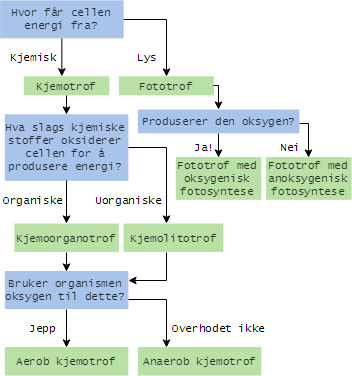
\includegraphics[width=0.45\textwidth]{metabolicdiversity}
	\caption{Klassifisering av organismer, basert på energikilde.}
	\label{fig:metabolicdiversity}
\end{figure}

\paragraph{Energibærere} Energivalutaen i celler er \emph{Adenosin trifosfat} (\ix{ATP}). ATP er det som produseres når cellen bryter ned næringsstoffer, og det som brukes når cellen skal gjøre noe som krever energi. Reaksjonen der ATP mister en fosfatgruppe for å bli adenosin difosfat (ADP) slipper løs 32 kJ/mol. De samme gjelder \ce{ADP -> AMP}. \ce{AMP ->}Adenosin slipper løs 14 kJ/mol når fosfat-adenosin-bindingen kuttes. Ett vannmolekyl inngår i hver slik spaltning.

\paragraph{Elektronbærere} Energibærere som overfører elektroner: nikotinamid adenin dinukleotid (\ix{NAD}) og flavin adenin dinukleotid (\ix{FAD}).

\paragraph{Langtidslagring av energi} Gjøres ved å lagre stoffer som uløselige polymerer som kan oksideres for å generere ATP. Noen eksempler er \ix{glykogen}, polyhydroksyalkanoater og svovel i prokaryoter; og stivelse og fettsyrer i eukaryoter.

\paragraph{Anabolisme} Den delen av metabolismen som lager cellens byggestoffer fra enklere stoffer gjennom energikrevende reaksjoner.

\paragraph{Cellens byggestoffer} er 
\begin{itemize}[nolistsep,noitemsep]
	\item karbohydrater (består av monosakkarider som glukose og fungerer som energilager samt en komponent i cellevegger),
	\item nukleinsyrer (består av nukleotider, brukes til å lagre, transportere og uttrykke genetisk informasjon),
	\item proteiner (består av aminosyrer, brukes til enzymer, som strukturelle komponenter og til transport av molekyler), og
	\item lipider (består av glyserol, fettsyrer og i noen tilfeller fosfat, fungerer som membraner (enten cytoplasmamembranen eller intracellulære kompartmenter)).
\end{itemize}

\paragraph{Aerob glukosemetabolisme} Aerob \ix{glukosemetabolisme} er cellens mest effektive metode for å produsere ATP. Det kalles også respirasjon, og involverer den vanlige reaksjonen for celleånding:
\begin{equation*}
	\ce{C6H12O6 + 6O2 ->[\text{38 ADP til ATP}] 6CO2 + 6H2O}
\end{equation*}

\paragraph{Anaerob glukosemetabolisme} Kalles fermentering, og involverer reaksjoner som 
\begin{equation*}
	\ce{C6H12O6 ->[\text{1-4 ADP til ATP}] 2C2H5O2 + 2CO2}
\end{equation*}
Det produseres mye mindre cellemasse gjennom fermentering enn ved respirasjon (kun 5\%). Reaksjonen krever mer glukose per ATP som blir produsert, og produserer sideprodukter som etanol. Eksempler på anaerob glukosemetabolisme er gjæring, og er når menneskekroppen danner melkesyre.

\paragraph{Gjæring} Når konsentrasjonen av \ce{O2} blir lav, endres genuttrykket i gjær slik at det er andre enzymer som aktiveres. I stedet for enzymene som utfører aerob metabolisme, aktiveres enzymene som utfører anaerob metabolisme. Dette er prinsippet bak gjøring.

\paragraph{Metabolsk spor} Et metabolsk spor er en tegning av veien fra næringsstoff til produkt, med piler mellom mellomprodukter. Skissering av metabolske spor med glukose som utgangspunkt sies å være veldig eksamensrelevant. 

\paragraph{Glukosemetabolisme} Figur \ref{fig:glucose} er en omformulering av figuren på slides, og kan med fordel pugges siden detaljer herfra har vært eksamensoppgaver. Det er naturligvis en del forenklinger her, blant annet forklares det ikke hvor man får vann fra. Man blir ikke så fryktelig klok på hvorfor glukosemetabolisme er relevant for resten av stoffet ved å se på denne figuren. Det blir man derimot ved å se på den utvidede figuren i Box 1.4 i Renneberg; når du er ferdig med å lese hele pensum kan du stirre lenge og vel på den figuren, og innse at nesten alle bioproduktene som har blitt diskutert til syvende og sist stammer fra nedbrytning av glukose.

\begin{figure}[H]
	\centering
	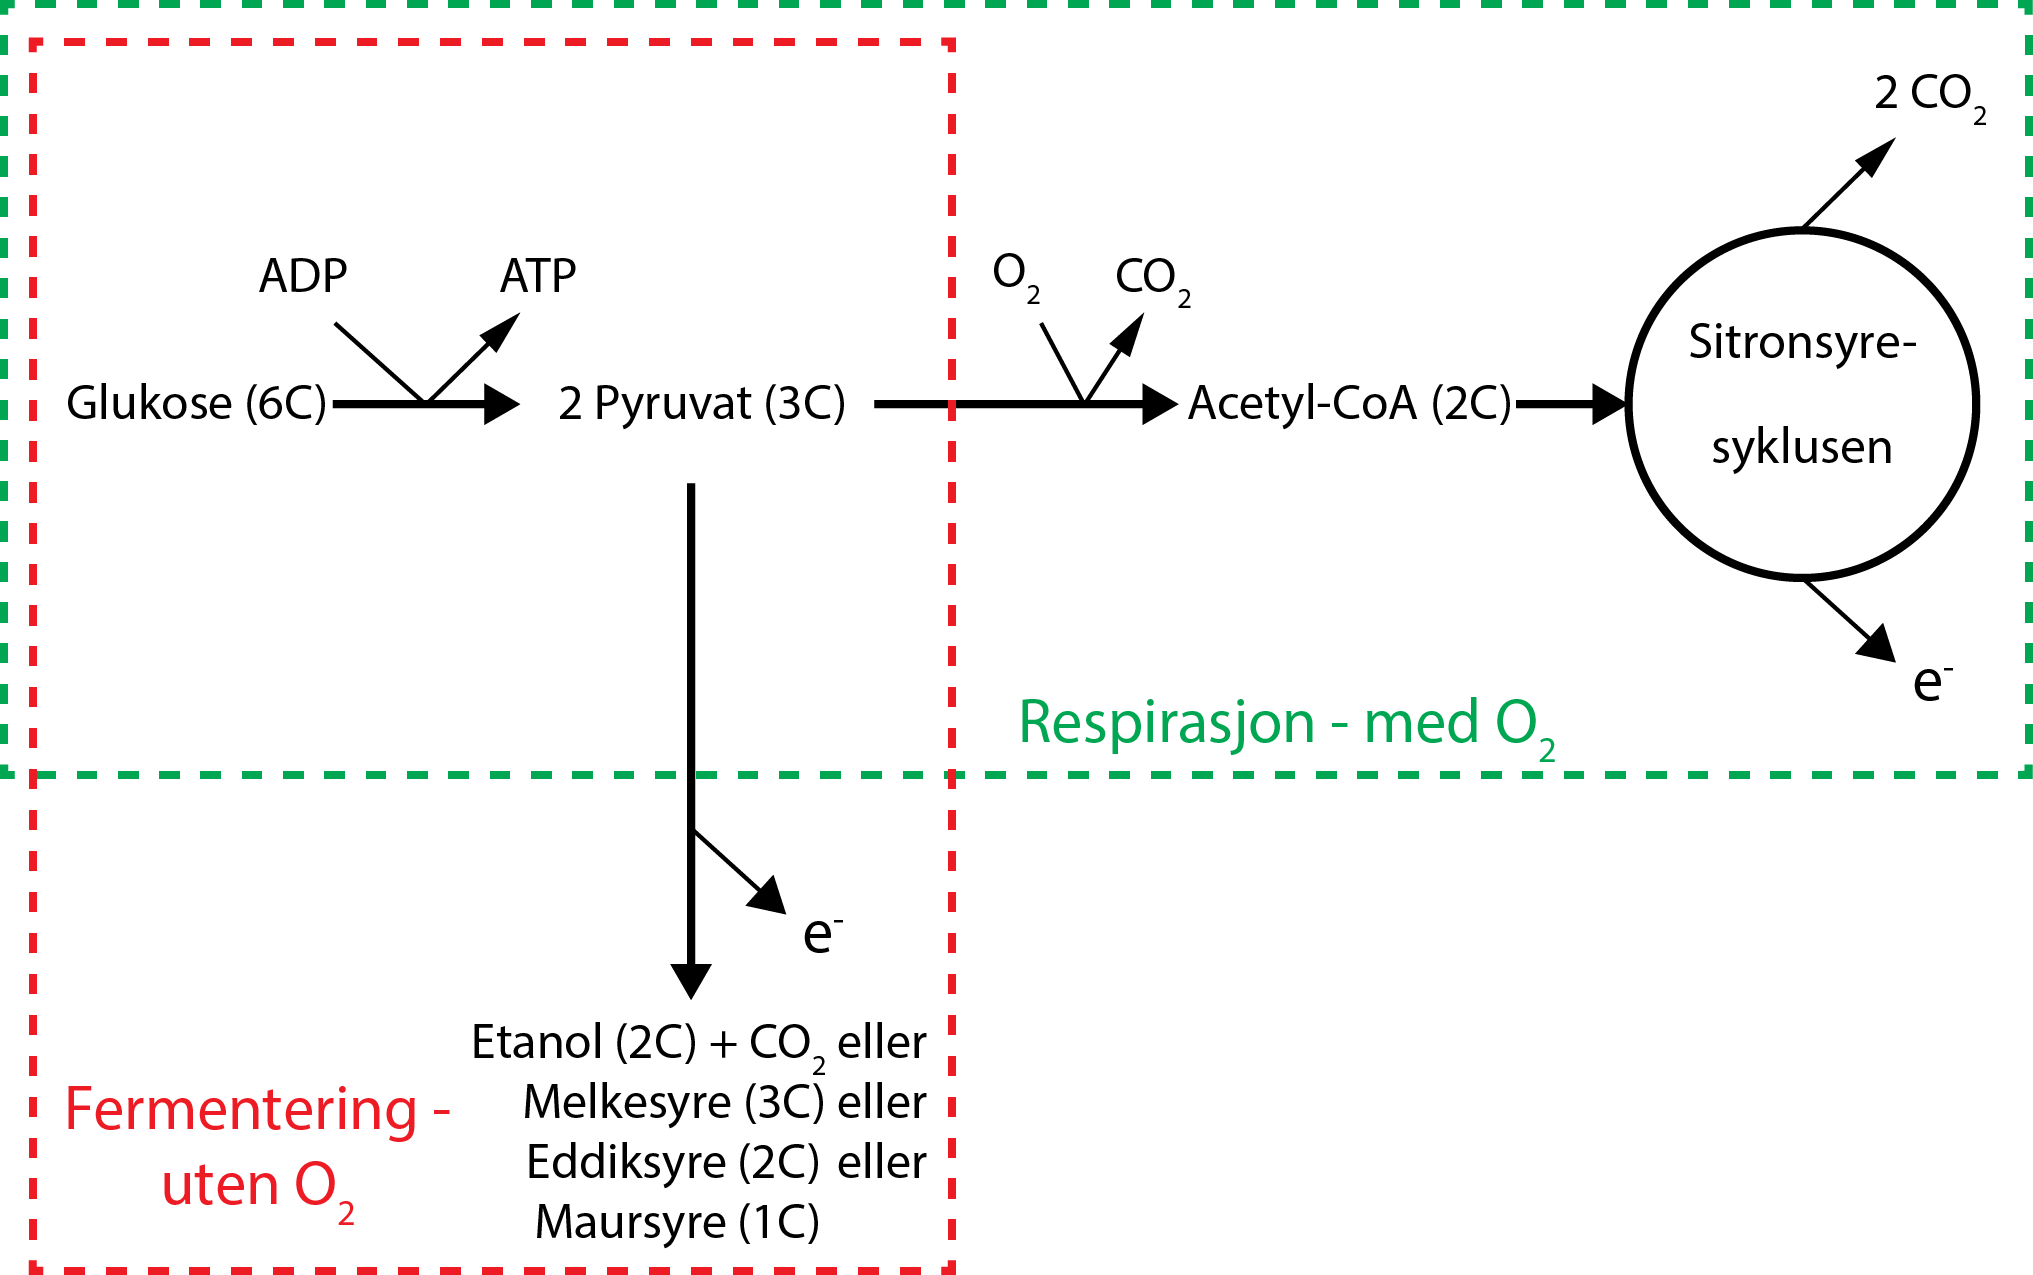
\includegraphics[width=0.45\textwidth]{glucose}
	\caption{Oversikt over glukosemetabolismen}
	\label{fig:glucose}
\end{figure}


\ctitle{Enzymer}

\paragraph{Dette kapittelet} forklarer hva proteiner er laget av og hvordan de er bygd opp. Så går vi nærmere på enzymer og hvordan de fungerer. Mot slutten også noen eksempler på enzymer, enzymkatalyserte reaksjoner og bioteknologiske løsninger som tar i bruk enzymer.

\cstitle{Proteiner} \index{proteiner}

\paragraph{Aminosyrer}\index{aminosyrer} Karbon bundet til et hydrogenatom, en karboksylsyregruppe og en aminogruppe, samt en såkalt R-gruppe som kan være mye rart (upolar alifatisk som i glysin, aromatisk som i fenylalanin, polar uladd som i serin, positivt ladd som i lysin, negativt ladd som i aspartat). 9 av de 20 aminosyrene som brukes i proteinsyntese er \ix{essensielle aminosyrer} som må opptas gjennom mat. 

\paragraph{\ix{D- og L-stereoisomeri}} En type \ix{stereoisomeri} for aminosyrer, som fungerer som følger: hvis man lar hydrogenatomet gå inn i arket, har man L-formen hvis gruppene som går mot klokka er \ce{COOH -> R -> NH_2}, og D-formen hvis man får denne rekkefølgen ved å gå med klokka.
\begin{center}
	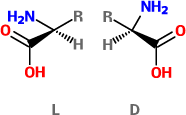
\includegraphics[scale=0.5]{enantiomers.png}
\end{center}
Av en eller annen grunn finnes kun L-enantiomerene til aminosyrene i proteiner. D-aminosyrer finnes andre steder i naturen, der de fungerer som mellomtrinn i aminosyremetabolisme, i polypeptider i celleveggene til noen bakterier, og som nevrotransmittere (signalstoffer). Det har også blitt syntetisert proteiner av D-enantiomerer i laboratoriet - disse vil være speilbilder av proteinene som dannes fra L-enantiomerene.

\paragraph{Peptidbinding} Aminosyrer bindes sammen via peptidbindinger i lange polymerer som vi kaller proteiner. En \ix{peptidbinding} dannes gjennom en kondensasjonsreaksjon når \ce{H} fra en aminogruppe og \ce{OH} fra en karboksylsyregruppe går ut som et vannmolekyl, og legger igjen en binding som ser slik ut:
\begin{center}
	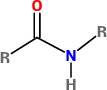
\includegraphics[scale=0.5]{peptide}
\end{center}
På grunn av \ix{resonans} i peptidbindingen (i resonansstrukturen som ikke er vist i figuren, blir \ce{C=O}-bindingen til en \ce{C-O^-}-binding, mens \ce{C-N}-bindingen blir til en \ce{C=N^+}-binding) kan ikke molekylet rotere rundt en peptidbinding, og alle atomene som inngår i en peptidbinding (C, O, N, H) ligger i samme plan.

\paragraph{Peptider} Korte kjeder av aminosyrer kalles \ix{peptider} og navngis ved å begynne på den terminale aminogruppen, traversere peptidet til man støter på den terminale karboksylsyregruppen, og ramse opp alle aminosyrene på veien. Fullstendig navngivning av proteiner er dermed upraktisk, men det som er så fint er at det finnes altså en russisk fyr som har uttalt hele det fullstendige systematiske navnet til verdens lengste protein (\ix{titin}). Det tok så lang tid at man kunne se forskjellen i skjeggvekst på starten og slutten av opptaket.

\paragraph{Primærstrukturen til proteiner}\index{primærstruktur} er sekvensen av aminosyrer, samt eventuelle disulfidbindinger mellom cysteingrupper. Primærstrukturen gir opphav til sekundær- og tertiærstruktur (men du blir ikke akkurat så mye klokere på høyere ordens struktur ved å se på aminosyresekvensen). 

\paragraph{Sekundærstrukturen til proteiner}\index{sekundærstruktur} er lokale strukturer i proteinet. Det er bare to slike strukturer vi snakker noe særlig om: $\alpha$-helikser og $\beta$-flak.

\paragraph{\ix{$\alpha$-heliks}} Proteinet kan kveile seg i en spiral, som kan være venstre- eller høyrehendt. Denne strukturen stabiliseres av hydrogenbindinger langs spiralens akse. I en slik spiral kan man for eksempel ha at en side er hydrofob, mens den andre er hydrofil.

\paragraph{\ix{$\beta$-flak}} Flak som dannes når rette ``tråder'' av proteinet bretter seg frem og tilbake, med hydrogenbindinger mellom trådene. Hvis trådene går i samme retning, er flaket parallelt, og hvis de går i alternerende retninger er flaket antiparallelt. $\beta$-flak er foldet i ``trekkspill-mønster'', og R-gruppene på aminosyrene vil stå ut av flaket.

\paragraph{Tertiærstrukturen til proteiner}\index{tertiærstruktur} er den tredimensjonale strukturen som reflekterer proteinets funksjon. Slik struktur er stabilisert av hydrofobe interaksjoner med vann (hydrofobiske grupper vender seg mot midten av proteinet og hydrofile grupper vender seg utover) samt hydrogenbindinger og ioniske interaksjoner som optimaliseres i de mest termodynamisk stabile strukturene. Disse interaksjonene gjør at proteiner har en tendens til å ``krølle seg sammen'' til den karakteristiske klumpete formen.

\paragraph{Kvartærstrukturen til proteiner}\index{kvartærstruktur} I noen tilfeller er det flere proteiner, eller flere molekyler av det samme proteinet, som går sammen for å danne en større struktur. Denne strukturen kalles da kvartærstrukturen til proteinet. Et eksempel på et protein med kvartærstruktur er \ix{hemoglobin}, der 4 polypeptidkjeder går sammen for å danne én funksjonell enhet.

\cstitle{Enzymer}

\paragraph{Enzym}\index{enzym} Biologisk katalysator som får reaksjonene i cellen til å gå raskere ved å senke aktiveringsenergien til reaksjonene.

\paragraph{Struktur til enzymer} De fleste enzymer er proteiner. Det finnes også enzymer som består helt eller delvis av RNA, disse kalles \ix{ribozym}er. Proteiner er bygget opp av aminosyrer som er kovalent bundet til hverandre i lange kjeder. Et område på en enzym der det foregår en reaksjon kalles et \idx{aktivt sete}.

\paragraph{Substrat} Enzymer er gjerne veldig spesifikke, i så stor grad at proteinet har en fysisk form der molekylet som skal prosesseres (dette molekylet kalles \idx{substrat}et) passer inn. 

\paragraph{Nøkkel-i-lås}\index{nøkkel-i-lås} Dette var den første hypotesen om samspillet mellom enzymet og substratet: at substratet passer perfekt inn i enzymet fordi enzymet er en romlig negativ av substratet. En slik hypotese forklarer hvordan enzymer kan være så spesifikke.

\paragraph{Hånd-i-hanske}\index{hånd-i-handske} Det har vist seg at substratet fungerer mer som en hånd i en handske, fordi substratet og enzymet kan påvirke hverandre underveis i reaksjonen. Enzymet og substratet er altså litt mer fysisk fleksible enn nøkkel-i-lås-analogien skulle tilsi.

\paragraph{Lysozym}\index{lysozym} er det første proteinet som ble analysert ned til den minste atomære detalj. Lysozym hydrolyserer bindingen mellom sukkerring 4 og 5 i et molekyl som består av 6 sukkerringer. 

\paragraph{Glukoseoksidase} Dette proteinet omformer $\beta-D$-glukose, men ingen andre sukkerarter eller karbohydrater, til glukonolaton. Dette er fordi det kun er $\beta-D$-glukose som er lite nok og passer akkurat inn i den romlige strukturen til \ix{glukoseoksidase}. Glukoseoksidase er med andre ord svært \ix{substratspesifikt enzym}.

\paragraph{Mulige årsaker til \ix{reduksjon i aktiveringsenergi}} Enzymer kan redusere aktiveringsenergien til en reaksjon. Enzymet binder seg ikke til substratet i sin opprinnelige konfigurasjon, men til en mellomtilstand som kan være deformert i forhold til det originale stoffet.

Inne i enzymet er svært reaktive funksjonelle grupper konsentrert på et veldig lite område, og satt sammen på en måte som gjør at de er i direkte kontakt med bindingene i substratet som skal modifiseres. Området rundt det aktive setet består stort sett av upolare grupper, som gjør at enzymet lokalt ligner på en organisk (upolar) løsning. Dermed blir de få polare gruppene i nærheten svært reaktive i forhold til det de ville vært i vandig løsning.

\paragraph{Kofaktorer}\index{kofaktor} Kjemiske stoffer som ikke er proteiner, og som et enzym krever for å utføre oppgaven sin. Typisk inorganiske molekyler som \ce{Fe^3+}, \ce{Mg^2+}, \ce{Mn^2+} og \ce{Zn^2+}.

\paragraph{Koenzymer}\index{koenzym} Organiske forbindelser som binder seg til eller i nærheten av det aktive setet. De modifiserer strukturen til substratet eller beveger elektroner, protoner eller kjemiske grupper mellom substratet og enzymet. I motsetning til enzymene selv brukes koenzymer opp i enzymkatalyserte reaksjoner. Mange av disse kommer fra vitaminer, for eksempel NAD$^+$ fra vitamin B.

\paragraph{Klassifisering av enzymer} Det finnes seks typer enzymer, som navngis etter hva de gjør:
\begin{itemize}[nolistsep,noitemsep]
	\item \idx{oksidoreduktaser} reduserer ett stoff og oksiderer et annet,
	\item \idx{transferaser} overfører kjemiske grupper fra et stoff til et annet (gjerne ved hjelp av koenzymer),
	\item \idx{hydrolase}r kløyver stoffer med addisjon av vann,
	\item \idx{lyaser} kløyver stoffer uten addisjon av vann (og danner gjerne dobbeltbindinger eller ringstrukturer),
	\item \idx{isomeraser} omdanner et molekyl til en annen isomer, og 
	\item \idx{ligaser} bruker ATP for å binde sammen to stoffer.
\end{itemize}

\paragraph{Eksempler på enzymer og \ix{enzymkatalyserte reaksjoner}}
\begin{itemize}[noitemsep,nolistsep]
	\item \emph{Ekstracellulære hydrolaser}\index{hydrolase} produseres av mikrober og slippes ut i miljøet for å degraderer biopolymerer til mindre enheter som kan tas opp av mikroben. De brukes også av edderkopper til såkalt ekstraintestinal fordøyelse. Ekstracellulære hydrolaser er av naturlige grunner de enzymene som er enklest og billigst å ekstrahere fra en cellekultur - det er ikke noen cellemembran mellom deg og enzymet. De fire neste eksemplene er \ix{ekstracellulære hydrolaser}.
	\item Malt inneholder \idx{amylaser}, som bryter opp stivelse til kortere oligosakkarider, samt glucoamylase, som bryter opp oligosakkarider til glukose. Disse enzymene kan brukes i baking for å bryte ned stivelse til sukker og dermed akselerere heving, samt for å degradere klebrig gluten og gjøre deigen luftigere. I tekstilindustrien tilsetter man gjerne stivelse for å få fibrene til å holde seg sammen under veving. Amylaser brukes til å fjerne stivelse når vevingen er ferdig.
	\item \emph{Pektinaser}\index{pektinase} bryter ned de store pektinmolekylene i frukt for å gjøre juicen mindre tyktflytende. Hvis man ikke fjerner pektin, får juicen en gel-aktig konsistens som er uønsket og vanskelig å håndtere. Pektinaser hentes fra \idx{Aspergillus}- og \idx{Rhizopus}-sopp.
	\item Papaya, fiken og ananas inneholder \idx{proteaser} som bryter ned bindevev i kjøtt, og dermed gjør det mørere. De samme enzymene brukes også for å mykne lær. 
	\item \emph{Hydrolaser med lav substratspesifisitet}: brukes som vaskemidler som bryter ned fett og proteiner, som binder seg til fibrene i tøy. Fett og proteiner er ``limet'' som gjør at skitt setter seg fast i klær. Enzymer er nyttige fordi de gjør at man kan gjøre oppvasken på relativt lav temperatur. Før i tida måtte slike enzymer hentes ut fra bukspyttkjertler til dyr, men etter at enzymet \ix{subtilisin} ble oppdaget i \idx{Bacillus licheniformis}  på 60-tallet, inneholder vaskemiddel som regel hydrolytiske enzymer fra mikroorganismer. Andre enzymer som brukes i vaskemiddel er cellulaser, som bryter ned mikrofibre i bomull og gjør stoffet mer mykt, og amylaser og lipaser som fjerner matrester i vaskemaskiner.
	\item Fosfor i planter lagres gjerne i form av fytat, en seksringet forbindelse. Mennesker og dyr klarer ikke å ta opp fosfor i denne formen, men det finnes mikrobiell \idx{fytase} som hydrolytisk kløyver fytat slik at man ender opp med fosfat, som vi kan ta opp. Fytaser er et spesielt nyttig tilskudd i grisefôr, fordi man slipper å tilsette så mye miljøskadelig fosfat (kapittel 6) i fôret.
	\item \emph{Glukoseisomerase}\index{glukoseisomerase}: brukes til å omdanne glukose til fruktose, som er søtere enn glukose (og sukrose). 
\end{itemize}

\paragraph{Immobiliserte enzymer}\index{immobilisering} Enzymer som på en eller annen måte sitter fast i et medium. Metoder for å immobilisere enzymer inkluderer adsorbsjon til fibre, kovalente bindinger til fibre, krysslinking mellom enzymer, immobilisering i gel eller hule fibre og mikrokapsler. 

Det som er fint med immobiliserte enzymer, er at de kan utføre reaksjoner under kontrollerte betingelser uten å legge igjen enzymrester i produktet (nyttig for å forhindre immunreaksjoner i pasienter). Samtidig blir mindre av enzymet kastet bort; enzymet er resirkulerbart. 

\paragraph{Enzymkilder}\index{enzymkilder} Hvis vi vil ha tak i enzymer til eget bruk, har vi forskjellige kilder. Av det som ikke er nevnt tidligere: Bukspyttkjertler, spesielt til gris, inneholder mye fint: trypsin, chymotrypsin, lipaser og amylaser. Magesekker inneholder pepsin. En av de nyttigste enzymkildene er mikroorganismer, som er veldig greie å ha med å gjøre og kan gros på laben og i reaktorer - og via genteknologi kan enzymene skreddersys. Det finnes også mange bruksområder for enzymene som dannes av ekstremofile mikroorganismer, for eksempel DNA polymerase, som vi skal se blir nyttig i analytisk bioteknologi (kapittel 10).

\setcounter{section}{9}
%!TEX root = Nanomat.tex
\ctitle{Katalyse med metall-nanopartikler}
\paragraph{Poenget med metall-nanopartikler} Metall-nanopartikler er særlig brukt til katalyse, og lages ofte av kostbare metaller som palladium, sølv, platina eller gull. Siden katalyse (i likhet med alle andre kjemiske reaksjoner) skjer på overflaten av materialet, ønsker vi at katalysatorene skal bestå av så mye overflate som mulig\footnote{Så mye overflate som mulig, og så lite dybde som mulig. Akkurat som dette emnet! ZING!} - derfor vil vi ha metallene i form av nanopartikler.

\cstitle{Størrelseseffekter}
Størrelseseffekter refererer til endringene i metallets egenskaper når partiklene det består av er veldig små. Igjen: størrelseseffekter forårsakes av to ting:  \emph{økt andel atomer med lavt koordinasjonstall} \emph{endring i elektronstruktur/kvantemekaniske effekter}.

\paragraph{Økt andel atomer med lavt koordinasjonstall} Katalyse skjer, veldig forenklet, i to trinn:
\begin{enumerate}
	\item Reaktantene adsorberes på overflaten av katalysatoren, og bindingene i reaktantene brytes der.
	\item Reaktantene reagerer med hverandre og desorberes fra katalysatoren.
\end{enumerate}
Når katalysatorene er i form av bittesmå partikler, kan det medføre både fordeler og ulemper. Siden vi har mange reaktive atomer, er det lettere å få til trinn 1. Men det blir også vanskeligere å få til trinn 2. Hvis vi ikke får til trinn 2, vil katalysatoren raskt bli dekket med reaktant, og reaksjonen vil opphøre.

\paragraph{FCC-nanopartikler} FCC\footnote{Den riktige/vanlige måten å skrive forkortelser for krystallstrukturer på, er å bruke små bokstaver, altså ``fcc'' i stedet for ``FCC''. Personen som fant på denne konvensjonen lever ikke lenger, jfr. fotnote 15.}-strukturen er tettpakket, og i bulkmaterialet har hvert atom et koordinasjonstall på 12. Wullf-polyederet til FCC-strukturen er et avstumpet oktaeder, og det er slik FCC-partikler ser ut når de blir tilstrekkelig store.

Noen FCC-metaller, som kobber og sølv, foretrekker å danne et ikosaeder (som er en ikke-krystallin struktur) når partiklene består av færre enn ca. 100 atomer, mens palladium, platina og gull danner avstumpede oktaedere allerede ved et noen titalls atomer.

En ting som kan være viktig å få med seg om FCC-nanopartikler er at overflateatomer med samme koordinasjonstall ikke nødvendigvis har samme elektroniske miljø:
\begin{itemize}
	\item overflateatomet som er nabo til en kant, har et annet miljø enn overflateatomet som er midt i en flate.
	\item et atom på en kant mellom to $(111)$-plan har et forskjellig elektronisk miljø fra et atom på en kant mellom et $(100)$-plan og et $(111)$-plan.
\end{itemize}

\paragraph{Effekter ved overflaten} Ved overflaten skjer det flere spennende ting:
\begin{itemize}
	\item Avstanden mellom to atomer på overflaten er mindre enn avstanden mellom to atomer i bulk.\footnote{Man kan kanskje se på det som at atomene prøver å gjøre opp for de tapte bindingene sine ved å binde seg sterkere til atomene som er igjen.} 
	\item Atomene på overflatene trekker seg også sammen med atomene rett under seg. Jo lavere koordinasjonstall atomet på overflaten har, jo mer trekker det seg inn mot atomene under seg. Dette har blitt vist i nikkel: på det tettpakkede $(111)$-planet er avstanden mellom ytterste og nest ytterste atom 1-2\% mindre enn gitterparameteren. På det mindre tettpakkede $(111)$-planet er denne sammentrekningen nærmere 10\%.
	\item Hvis det adsorberes reaktanter på overflaten av nanopartiklene, vil det ikke lenger være løse bindinger der. Derfor vil adsorberte reaktanter forminske de ovennevnte effektene.
\end{itemize}

\paragraph{Endring i smeltepunkt, Lindemannkriteriet} Lindemannkriteriet er en definisjon av smelting: at man regner et (bulk)material som smeltet når de interatomære avstandene fluktuerer med mer enn 10\% av gitterparameteren. Siden atomer på overflaten er friere til å bevege seg enn de i bulk, vil en større andel overflateatomer føre til at dette kriteriet oppnås ved en lavere temperatur enn i bulkmaterialet. Dermed er smeltepunktet lavere for små partikler.

Et eksempel på konsekvensene av dette er produksjon av karbonnanorør med \ce{Ni}-nanopartikler som katalysator. Hvis man kjører denne prosessen ved \SI{800}{\celsius} får man en ganske annen morfologi enn hvis man gjør det ved \SI{700}{\celsius}. Forklaringen på dette er at smeltepunktet for de katalyserende nanopartiklene er et sted mellom disse temperaturene.

\cstitle{Endringer i elektronisk struktur}
For bulkmaterialer brukes \emph{valensbånd} og \emph{ledningsbånd} for å skille mellom metaller, halvledere og isolatorer. Forutsetningen for å kunne bruke en slik modell, er at man har et tilnærmet uendelig antall atomer, og at disse påvirker hverandres elektronstruktur. Den samlede effekten av alle disse gjensidige elektroniske påvirkningene er at det oppstår utallige forskjellige energinivåer som hvert enkelt elektron i materialet kan ``velge mellom''. Vi vet fra kvantemekanikken at det \emph{egentlig} bare finnes et endelig antall energinivåer for hvert elektron, men når materialet består av mange atomer, er tilnærmingen god. 

Tilnærmingen krever modifisering når nanopartiklene består av et antall partikler som ikke kan tilnærmes med uendelig. For det første: når partiklene blir små, minker bredden på energibåndene, og det begynner å oppstå energigap. Etter hvert blir de så tynne at materialer som i bulkform er metaller, blir til halvledere og til slutt elektriske isolatorer.  For det andre: når partiklene består av et ett- eller tosifret antall atomer, endres de elektroniske egenskapene plutselig og uforutsigbart avhengig av størrelse (se figur 10.5 i Bréchnigac). For å beskrive de elektroniske egenskapene til så små partikler, kreves en ordentlig kvantemekanisk analyse.

Et eksempel på ``bruk'' av størrelsesavhengig elektronisk struktur er fotoluminescens i \ce{CdSe}-nanopartikler med diameter på mindre enn \SI{10}{\nano\meter}. Slike partikler er halvledende, og har et energigap $E_g$ som avhenger av størrelsen på partikkelen. Hvis man lyser på partiklene, lyser partiklene tilbake med en viss farge. Fargen avhenger av $E_g$ og dermed altså av størrelsen på partiklene. Check it out:
\begin{figure}[H]
	\centering
	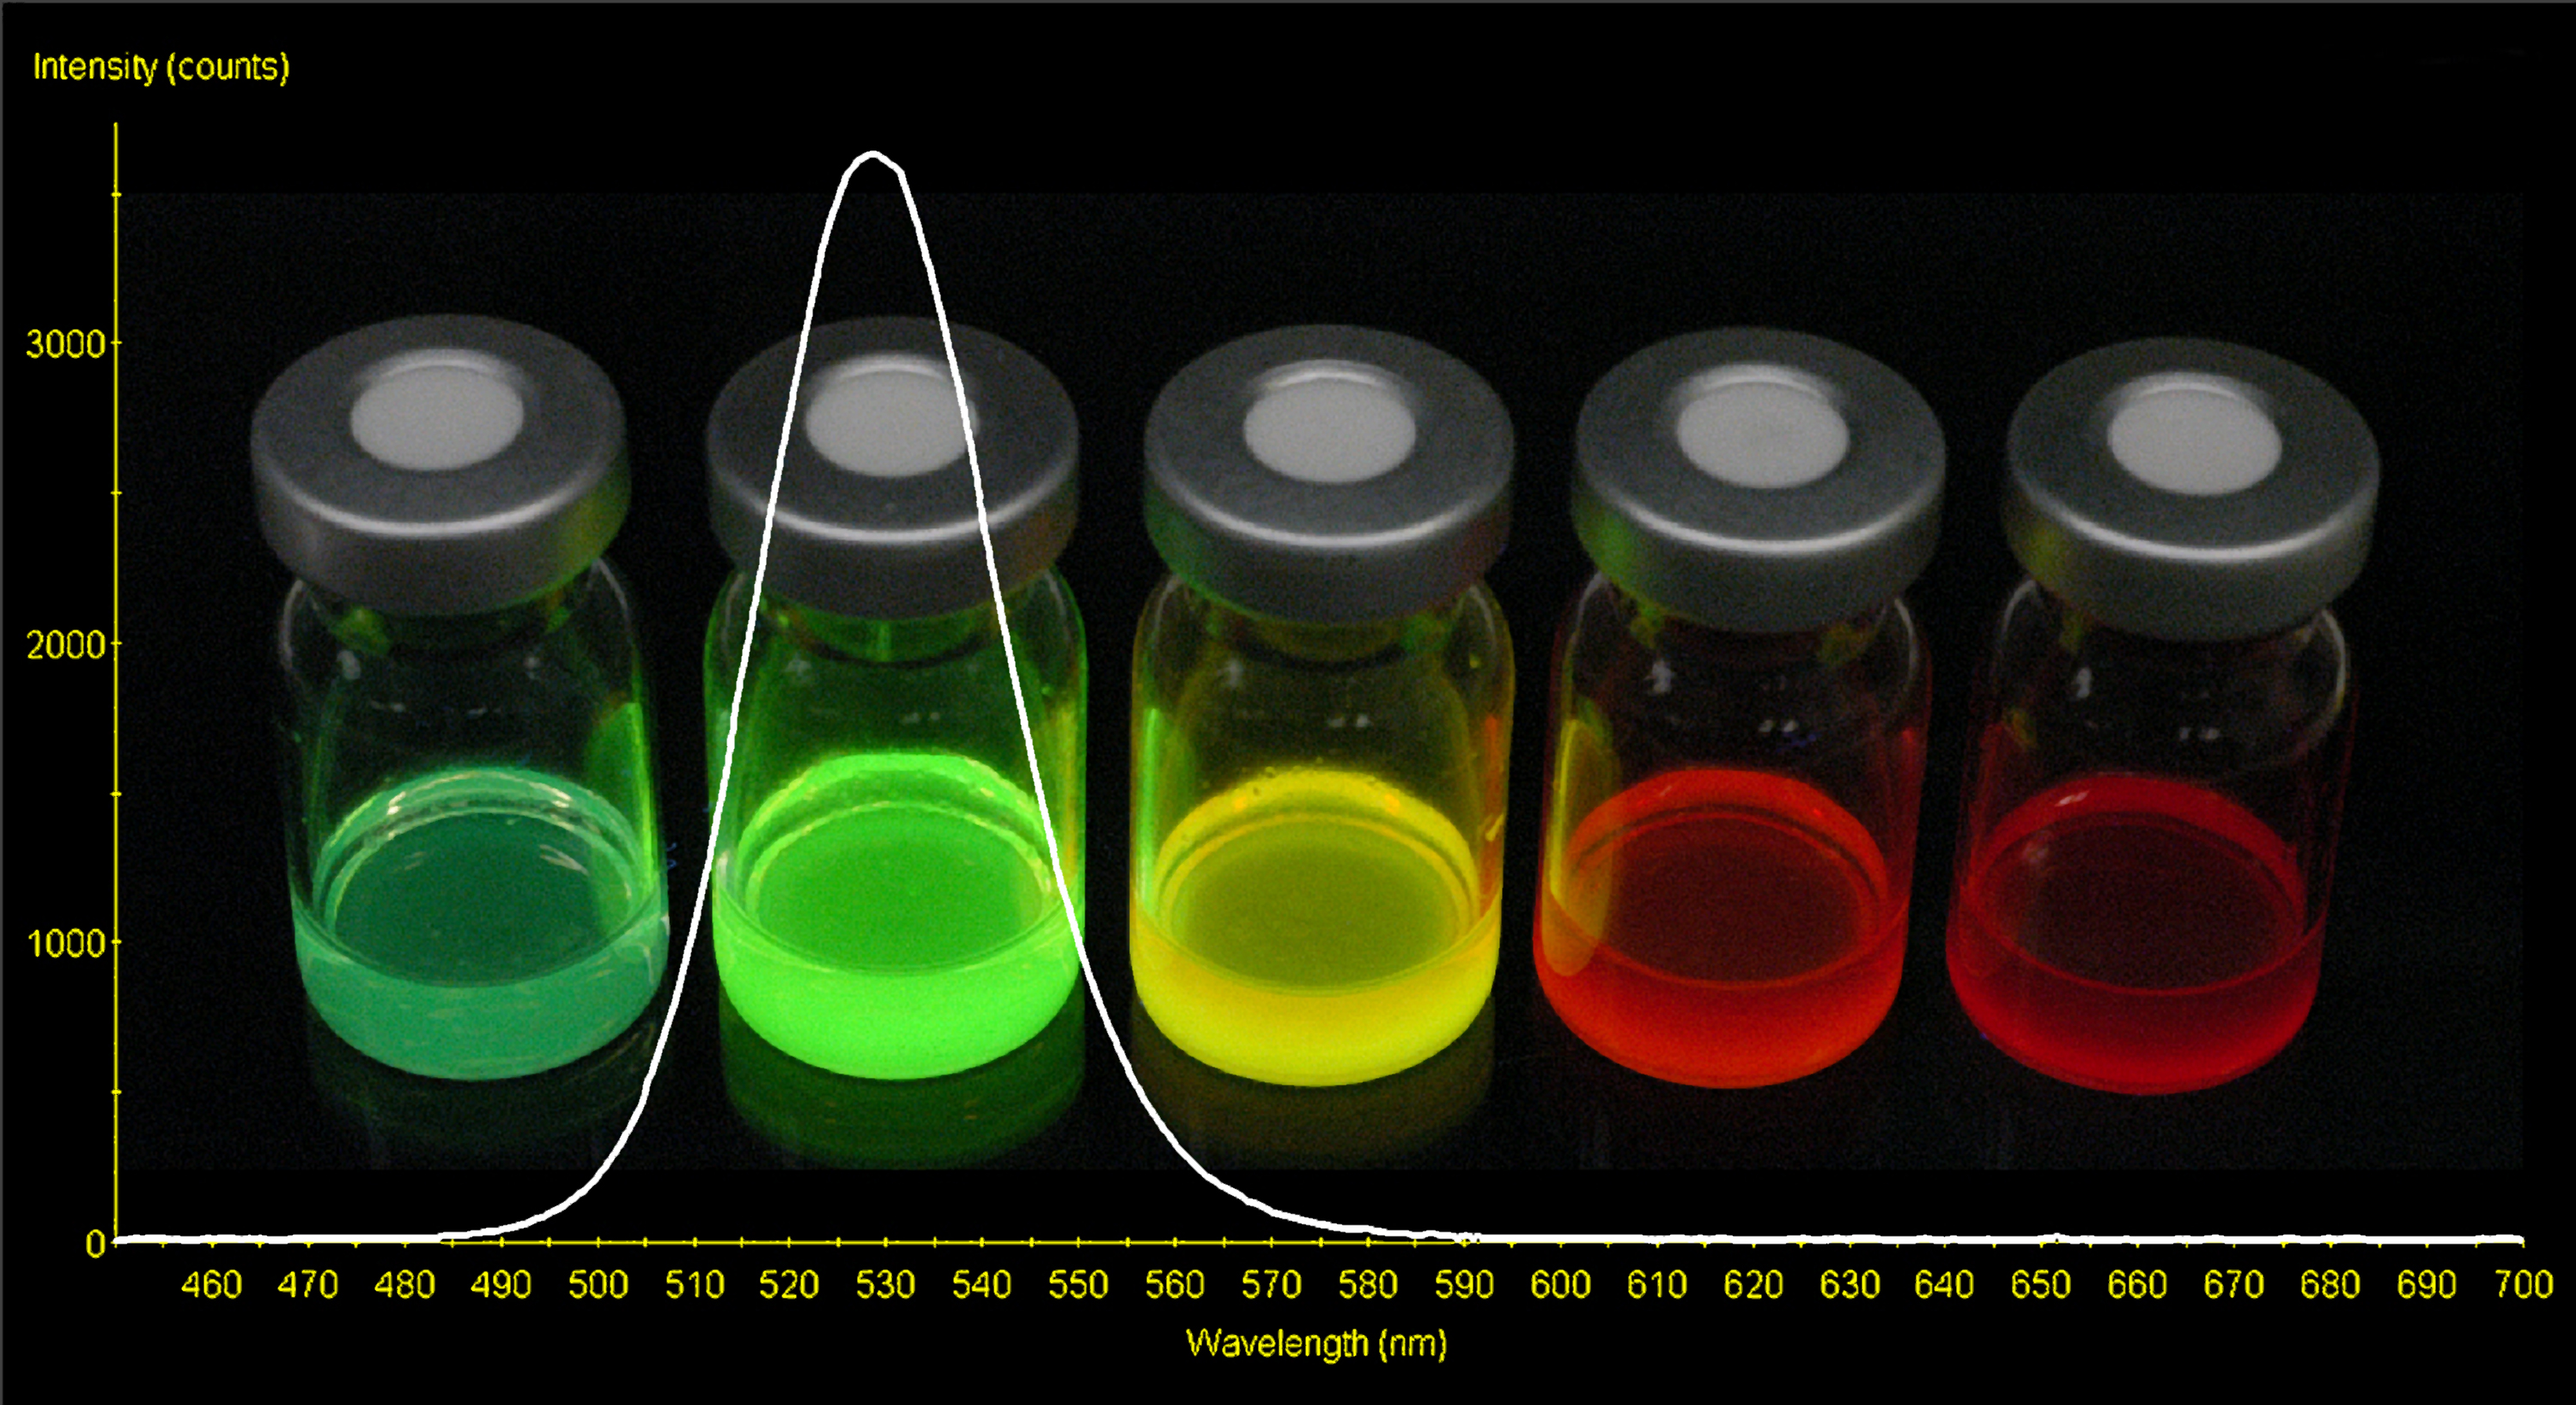
\includegraphics[width=0.95\linewidth]{CdSeqdots.jpg}
	\caption{\ce{CdSe}-kvanteprikker, av forskjellig størrelse, som har blitt bestrålt med UV-lys. Og en graf. Jeg tror grafen beskriver strålingen fra den grønne løsningen.}
	\label{fig:qdots}
\end{figure}

\cstitle{Legeringseffekter}
Egenskapene til katalysatoren kan endres når man legger til et annet metall. En legering av to metaller kan være en bedre katalysator enn begge metallene er hver for seg. Dette har å gjøre med ting som at det aktive setet på en katalysator består av mer enn ett atom, og at legeringer er komplekse greier.

\paragraph{Overflatesegregering} Det er gjerne slik at de atomene som har lavest overflatespenning beveger seg ut mot overflaten, for å minimere overflateenergien til partikkelen som helhet. Det vil særlig være større andel atomer med lav overflatespenning på fasettene som har lavt koordinasjonstall, og på kanter og hjørner. Hvis atomet attpåtil har stor atomradius, blir effekten enda sterkere.

Her er et eksempel på når det kan være nyttig. Man kan lage hydrogen i reaksjonen \ce{2H2O + CH4 -> CO2 + 4H2}, katalysert med \ce{Ni}. Men da pleier karbon å feste seg til nikkelatomene på kanter/hjørner og ikke gi slipp, slik at katalysatoren blir deaktivert og reaksjonen stopper etter kort tid. For å løse dette legger vi til litt \ce{Au}, for gull har lavere overflatespenning enn nikkel, og gullatomene vil bevege seg mot kantene og hjørnene. Karbonet binder seg ikke like bra til gull, så vi får en \emph{bedre katalysator} selv om vi har lagt til noen \emph{mindre reaktive} gullatomer.

Overflatesegregering kan begrenses dersom atomer av forskjellig type binder seg sterkere til hverandre, enn hver type atomer binder seg til hverandre hver for seg --- altså dersom
\begin{equation}
	\Delta H_{\ce{A-B}} > \frac{1}{2}\left(\Delta H_{\ce{A-A}} + \Delta H_{\ce{B-B}}\right).
\end{equation}
Effekten begrenses naturligvis også av at termisk energi mikser og trikser med atomene, ellers ville den minste forskjell i overflatespenning forårsaket fullstendig segregering for legeringer der ulikheten over ikke holder.

\paragraph{Fortynningseffekt} Noen katalytiske reaksjoner krever at man har en sammenhengende gruppe med flere atomer av samme type. Hvis overflaten fortynnes med andre atomer, vil det finnes færre slike steder, så disse reaksjonene vil skje sjeldnere. Andre reaksjoner, som \emph{ikke} krever en slik sammenhengende gruppe, vil ikke påvirkes i samme grad. Hvis det vi ønsker oss er reaksjoner av den sistnevnte typen, bør vi bruke en legering for å øke selektiviteten til katalysen.

\paragraph{Effekter på elektronisk struktur} Interaksjoner mellom de to metallene kan endre elektronstruktur gjennom ting som kjemisk binding, ladningsoverføring, polarisering og spenninger i krystallgitteret. Dette vil igjen påvirke reaktiviteten til det katalyserende metallet. Det er ofte vanskelig å finne ut hva som forårsaker hva.


%!TEX root = Nanomat.tex
\ctitletwo{NS8 Fullerener og karbonnanorør}
\addcontentsline{toc}{section}{NS8 FULLERENER OG KARBONNANORØR}
PR-avdelingen for karbon er veldig flinke. Når noen sier ``nano'', ser de fleste for seg en molekylmodell av grafen, et karbonnanorør eller en buckyball. La oss se litt på hvordan noen av tidenes mest hypede materialer fungerer.

\paragraph{Krystallstrukturer/allotroper for karbon} Det finnes en del forskjellige former for rent karbon.
\begin{itemize}
	\item Grafen: her er hvert karbonatom bundet til tre andre karbonatomer, med en vinkel på \SI{120}{\degree} mellom hver binding. Hvert atom er altså $sp^2$-hybridisert. Dette gir endimensjonale lag som er ett atom tykke.
	\item Grafitt: dette er mange lag av grafen pakket oppå hverandre, med svake bindinger på tvers av lagene. Siden lagene lett glir forbi hverandre, er grafitt mykt. Grafitt forekommer i naturen.
	\item Diamant: her er hvert karbonatom bundet til fire andre karbonatomer i en tetragonal sturktur. Hvert atom er altså $sp^3$-hybridisert. Denne krystallformen er ekstremt hard. Diamant forekommer i naturen som et mineral og er i utgangspunktet gjennomsiktig, men forurensninger kan farge materialet.
	\item Lonsdaleitt: dette er en tredje naturlig form for karbon som dannes ved meteorittnedlag.
	\item Fulleren: dette er når karbonatomene danner lukkede ``baller'', for eksempel det berømte Buckministerfulleren \ce{C60}. \ce{C60} er det minste stabile fullerenmolekylet, men det finnes også større fullerener. Der \ce{C60} ser ut som en fotball med en sekskant som grenser til hver side av hver femkant, har større fullerener flere sekskanter per femkant. Fullerener ble først oppdaget i 1985.
	\item Nanorør er litt som fullerener, men karbonatomene danner tuber i stedet for lukkede baller. Nanorørenes tykkelse på noen nanometer og lengde på noen mikrometer gir dem deres karakteristiske egenskaper. Nanorør kan enten være ``single-walled'' (SWNT på kort) eller ``multi-walled'' (MWNT). For MWNT's består tubene av flere lag utenpå hverandre. Nanorør ble oppdaget i 1991 i et forsøk på å lage fullerener.
	\item I tillegg er amorft karbon - karbon uten noen bestemt krystallstruktur - en ting som finnes.
\end{itemize}
\vfill
\cstitletwo{Fullerener}
\paragraph{Strukturen til fullerener} I alle stabile fullerener er hver femkant fullstendig omringet av sekskanter. Dette er grunnen til at \ce{C60} er det minste stabile fullerenet. De neste fullerenene som er stabile er \ce{C70}, \ce{C72}, \ce{C76}, \ce{C78} og \ce{C84}.

I \ce{C60} er alle karbonatomer ekvivalente. De inngår i to forskjellige typer bindinger: én dobbeltbinding (som skiller to sekskanter) og to enkeltbindinger (som skiller en femkant og en sekskant). Grunnen til at $\pi$-elektronene ikke er fullstendig delokalisert slik at alle bindingene blir ekvivalente, er krumningen til molekylet - bindingene i de $sp^2$-hybridiserte karbonatomene inngår i en pyramide, ikke i et plan. At bindingene ikke er i samme plan, gjør at \ce{C60} ikke er aromatisk.

Større fullerener er mindre symmetriske enn \ce{C60}, og karbonatomene vil være forskjellige (noen vil være i et hjørne mellom to sekskanter og en femkant, andre vil være i et hjørne mellom tre sekskanter).

\paragraph{Produksjon av fullerener} Fullerener produseres slik (se figur 8.4 i NS):
\begin{enumerate}
	\item Man har to grafitt-elektroder i en heliumatmosfære-
	\item De to elektrodene holdes i kontakt med hverandre. Den ene elektroden er veldig spiss, og kontaktflaten mellom de to elektrodene er veldig liten.
	\item Det sendes en strøm gjennom elektrodene. Siden arealet til kontaktflaten mellom elektrodene er veldig liten, blir også resistiviteten i dette området høy - dermed vil det bli svært høy temperatur i dette punktet på grunn av resistiv oppvarming. Denne høye temperaturen er \SIrange{2500}{3000}{\celsius}, høy nok til at grafitten fordamper og blir til plasma. 
	\item Grafitt-plasma kjøler ned i kontakt med helium-atmosfæren og danner et sotete råmateriale som består av fullerener, nanotuber og amorft karbon.
	\item Det er slik at fullerener av færre enn 100 atomer er løselige i aromatiske løsemidler, så disse kan isoleres med passende ekstraksjonsteknikker. Videre separasjon kan gjøres med kromatografi.
\end{enumerate}

\paragraph{Egenskapene til \ce{C60}} \ce{C60} er fullerenet som har blitt studert mest og best, så resten av diskusjonen av fullerener vil dreie seg rundt buckyballer:
\begin{itemize}
	\item Løselighet: \ce{C60} er uløselig i polare løsemidler og tungt løselig i hydrokarboner. De beste løsemidlene for \ce{C60} er aromatiske løsemidler som benzen, toluen og 1-kloronaftalen (der sistnevnte er desidert best).
	\item Fotofysiske egenskaper: \ce{C60} absorberer lys på en ikke-lineær måte; lys med lav intensitet absorberes lite, men hvis lyset er sterkere absorberes det bedre. Grunnen til dette har å gjøre med elektroniske tilstander og symmetri, og det er nok best å ikke tenke for mye på det. Effekten kan brukes til å beskytte optiske sensorer som kamera og øyne: \ce{C60} kan absorbere laserlys på avveie, men samtidig slippe gjennom belysningen i rommet.
	\item Elektrokjemiske egenskaper: \ce{C60} er en elektronakseptor og kan ta opp opp til 6 elektroner for å danne et stabilt \ce{C60^6-}-anion. \ce{C60} er lett å redusere og vanskelig å oksidere.
	\item Kjemiske egenskaper: mange derivater av \ce{C60} har litt laget ved å ``pode inn'' molekyler på overflaten av molekylet gjennom nukleofile addisjonsreaksjoner. Det vanligste er sykloaddisjon, altså at man lar en av kantene i \ce{C60} bli en del av en ring i reaksjonsproduktet. Slike reaksjoner gjøres ofte for å øke løseligheten til \ce{C60} slik at molekylet blir lettere å manipulere.
\end{itemize}

\cstitletwo{Karbonnanorør}
\paragraph{Strukturen til nanorør} Nanorør har som nevnt en lengde på noen mikrometer og en diameter på \SIrange{1}{10}{\nano\meter}. Krystallstrukturen er som et opprullet grafenlag (det er ikke nødvendigvis slik de oppstår, men det hjelper å tenke på det slik). I hver ende av nanorøret er det femkanter som fører til en krumning som lukker nanorøret. Nanorør kan ha tre forskjellige former, som avhenger av hvordan man ruller sammen grafenlaget (altså hvordan man kobler sammen sekskanter på motsatt ende avdet opprinnelige grafenlaget). De tre formene heter \emph{zigzag}, \emph{armchair} og \emph{chiral}, og forklares best ved å se på Figur 8.9 i NS.

% Kiral vektor, nevn hva m og n er

\paragraph{Elektronisk struktur for grafen og nanorør} Siden nanorør konseptuelt er laget ved å rulle opp grafen, kan de elektroniske egenskapene til nanorør utledes fra de elektroniske egenskapene til grafen. Dette gjøres ved hjelp av kvantemekanikk som er litt i overkant heftig for dette kurset, men det har seg slik at valensbåndet og ledningsbåndet er i kontakt med hverandre ved visse punkter i grafengitteret. Dette gjør grafen til et halvmetall.

Med litt mer av nevnte heftige kvantemekanikk viser det seg at
\begin{enumerate}
	\item Tuber i armchair-konfigurasjon er metalliske.\footnote{Jeg liker å huske dette ved å se for meg en skikkelig mettall type som sitter i en \emph{alt} for stor og myk ørelappstol.}
	\item Tuber i zigzag-konfigurasjon er metalliske hvis $n$ er et heltall ganger 3, og ellers halvledere.
	\item Tuber i kiral konfigurasjon er metalliske hvis $n-m$ er et heltall ganger 3, og ellers halvledere.
\end{enumerate}

\paragraph{Høy-temperatur-syntese av karbonnanorør} Det finnes to kategorier av metoder for å syntetisere karbonnanorør, som skilles fra hverandre ved hvilken temperatur syntesen gjøres ved. Høy-temperatur-syntese av karbonnanorør innebærer å \emph{sublimere grafitt} ved temperaturer som er høyere enn \SI{3200}{\celsius}, og deretter la karbonatomene kondensere i et område med en kraftig temperaturgradient. Høy-temperatur-syntese av karbonnanorør er ganske hardcore:
\begin{itemize}
	\item Du kan lage en kraftig elektrisk lysbue mellom to grafitt-elektroder, slik at det dannes et plasma med en temperatur på nærmere \SI{6000}{\celsius} ved anoden. Plasmaet farer bort til katoden og kondenserer der. Hvis katoden består av grafitt, får man kun MWNT's. For å få SWNT's må man også ha en metallkatalysator i katoden.\footnote{Lurer på hvorfor.}\footnote{Uansett, for å huske på dette liker jeg å se for meg at han mettall-fyren i ørelappstol er singel.}
	\item Du kan bombardere grafitt med høyenergetisk laserstråling. Hvis laserstrålingen ikke er kontinuerlig, men kommer i pulser, vil det dannes små klynger av karbon som kan bli til små SWNT's. Med kontinuerlig stråling kan man lage både MWNT's og SWNT's, da blir mekanismen omtrent den samme som hvis man skulle bruke elektrisk lysbue. For å lage MWNT's sikter man laseren på ren grafitt, for å lage SWNT's sikter man på grafen dopet med en metallkatalysator.
\end{itemize}
\vfill
\paragraph{Lav-temperatur-syntese av karbonnanorør: CVD} Hvis man ikke bruker høy nok temperatur til å sublimere grafitt, kalles metoden lav-temperatur-syntese. Metoden vi skal se på er ``Chemical Vapor Deposition'' (også kjent som CVD på kort, og som ``dette kommer vi tilbake til i kapittel 25'' på praktisk). Her er trinnene for CVD-produksjon av karbonnanorør:
\begin{enumerate}
	\item Du har en gass som inneholder karbon, f.eks \ce{CO} eller metan eller noe sånt, som er en kjemisk forløper til karbonnanorørene. Putt dette i en ovn med temperatur på 500-\SI{1000}{\celsius}.
	\item Du lar molekyler fra denne gassen brytes opp på overflaten av noen nanometer store metall-katalysator-partikler (av \ce{Fe}, \ce{Ni} eller \ce{Co}), slik at karbonet presipiterer på overflaten av partikkelen.
	\item Etter hvert som karbonet presipiterer, vil det danne nanorør! De kan være SWNT's eller MWNT's avhengig av reaksjonsbetingelser som temperatur, trykk og størrelse på nanopartikler. SWNT's får du med \emph{høy temperatur} og \emph{små metallpartikler}.\footnote{Så denne single fyren er \emph{hot}, men han har... små ``metallpartikler''? Nei, nå har denne huskeregelen gått for langt.}
\end{enumerate}
Mekanismen for hvordan tubene vokser, ligner veldig på mekanismen for VLS, som vi skal se på i ``Xia: Endimensjonale nanostrukturer''-kapittelet. Hvis du ikke har sett på dét kapittelet ennå kan du gjøre det nå, det er ganske gøy.

\paragraph{Egenskapene til nanorør} Nanorør har mange bra egenskaper:
\begin{itemize}
	\item \emph{Elektriske egenskaper}: De kan lede strøm ganske bra. Man kan oppnå en strømtetthet på så mye som \SI{10}{\giga\ampere\per\centi\meter\squared}, \footnote{\emph{10 gigaampere}! På halvparten av arealet til en femtiøring! Til sammenligning er strømmen som lager jordas magnetfelt, på 6 GA.} som er minst to størrelsesordener høyere enn man kan oppnå med metaller.
	\item \emph{Mekaniske egenskaper}: Grafitt er veldig stivt hvis du drar i en retning som ligger i planet, ellers er det ikke så veldig stivt. Tilsvarende er nanorør ekstremt stive hvis du drar på dem i lengderetningen\footnote{Knis.}, men de er også veldig lette å bøye, deformere og vri på\footnote{Æææ.}. Dette gjelder først og fremst SWNTs; MWNTs har ikke de samme elastiske egenskapene.
	\item \emph{Kjemiske egenskaper}: Man kan fylle nanorør med molekyler som fullerener eller andre ting for å lage fylte nanorør\footnote{``Fylte nanorør'' er forøvrig det som skal bli signaturretten når jeg avslutter min akademiske karriere for å starte en nanobasert temarestaurant! Den skal hete ``Nanomat''! Kickstarter-kampanje kommer snart.}. Man kan også putte molekyler på overflaten av nanorør.
\end{itemize}

\paragraph{Bruksområder for nanorør} Her er noen bruksområder for nanorør:
\begin{itemize}
	\item Man kan lage bittesmå ohmiske ledninger med dem.
	\item Man kan bruke dem som support for katalytiske metall-nanopartikler!
	\item Man kan bruke dem i solceller!
	\item Man kan putte dem på spissen av en AFM-probe for å få en mye spissere tupp som gir mindre konvolusjon!
\end{itemize}

\setcounter{section}{14}
\ctitle{Løsninger og blandinger}
\paragraph{Dette kapittelet} Kjemisk potensial forklarer også oppførselen til systemer som består av to forskjellige kjemiske specier, eller løsninger som danner faser med forskjellige konsentrasjoner av hvert specie. Her ser vi på $(T,V,N)$-ensemblet (det kanoniske) fordi det gir de enkleste gittermodellene. Derfor er størrelsen vi ønsker å minimere $F=U-TS$.

\cstitle{Entropi for blandinger}
Vi ser på en gittermodell med $N_A$ molekyler av type $A$ og $N_B$ molekyler av type $B$, slik at de $N=N_A+N_B$ molekylene fyller opp gitteret fullstendig. $A$ og $B$ antas å ha samme størrelse. I utgangspunktet er de adskilt med en vegg eller noe lignende, og deretter fjernes veggen slik at de to fasene blandes. Multiplisiteten til blandingen blir 
\begin{equation}
	W_{AB}=\frac{N!}{N_A!N_B!}
\end{equation}
Siden multiplisiteten til de ublandede systemene er 1, blir entropiendringen for blandingsprosessen lik den absolutte entropien til blandingen:
\begin{equation}
	\Delta S_{\text{mix}}=S_{AB}-(S_A+S_B)=S_{AB} = k_B\ln W_{AB}
\end{equation}
Denne entropien blir, med Stirlings formel:
{\small \begin{align}
	\Delta S_{\text{mix}} &=k_B\ln W_{AB} \\ &=k_B(N\ln N-N_A\ln N_A-N_B\ln N_B) \\
	&=k_B(N_A\ln N + N_B \ln N - N_A \ln N_A - N_B\ln N_B) \\
	&=-k_B(N_A\ln\frac{N_A}{N}+N_B\ln\frac{N_B}{N})
\end{align}}
Uttrykt ved molfraksjoner $x_j=\frac{N_j}{N}$ blir 
\begin{equation}
	\Delta S_{\text{mix}} = -k_B(N_A\ln x_A + N_B \ln x_B)
\end{equation}
Siden $x_B=1-x_A$, lar vi $x=x_A$ og får at
\begin{equation}
	\frac{\Delta S_{\text{mix}}}{Nk_B}=-x\ln x-(1-x)\ln(1-x)
\end{equation}

\cstitle{Ideelle løsninger}
Hvis vi ser bort ifra interaksjonene mellom partikler får vi at
\begin{equation}
	\Delta F_{\text{mix}}=-T\Delta S_{\text{mix}}
\end{equation}
Dette er analogt med forenklingen vi gjør når vi ser på en ideell gass. Å se bort i fra interaksjonene mellom partikler i kondensert fase er imidlertid helt urealistisk, så denne modellen bruker vi ikke videre.

\cstitle{Energi i blandinger}
Med samme gittermodell som i tidligere kapitler (kun nærmeste nabo-interaksjoner) blir
\begin{equation}
	\label{mixenergy}
	U=m_{AA}w_{AA}+m_{BB}w_{BB}+m_{AB}w_{AB}
\end{equation}
der $m_{XY}$ er antallet bindinger mellom en partikkel av type $X$ og en partikkel av type $Y$, og $w_{XY}$ er energien assosiert med en slik binding. Hver plass i gitteret har $z$ sider, så da er
\begin{align}
	zN_A&=2m_{AA}+m_{AB} \\
	zN_B&=2m_{AB}+m_{AB}
\end{align}
Grunnen til at en faktor 2 dukker opp i det ene leddet og ikke det andre, er at det totale antallet sider som grenser til en partikkel av type $A$ er 
\begin{align}
\begin{split}
	&\text{antall AA-bindinger}\times\text{2 A-sider pr. AA-binding} \\
	+&\text{antall AB-bindinger}\times\text{1 A-side pr. AB-binding}
\end{split}
\end{align}
og tilsvarende for $B$. Vi får at
\begin{align}
    m_A=\frac{zN_A-m_{AB}}{2} \\
    m_B=\frac{zN_B-m_{AB}}{2}
\end{align}
Da blir \eqref{mixenergy} til en funskjon av kun $m_{AB}$,
\begin{align}\begin{split}
	\label{mixenergy2}
	U=\\&\frac{zN_A-m_{AB}}{2}w_{AA}\\+&\frac{zN_B-m_{AB}}{2}w_{BB}\\+&m_{AB}w_{AB}
\end{split}\end{align}
Så må vi finne $m_{AB}$. Vi kan finne en tilnærming til den ved hjelp av Bragg-Williams-modellen.

\cstitle{Bragg-Williams-modellen}
I Bragg-Williams-modellen antar vi at partiklene er blandet så tilfeldig og uniformt som mulig, i samsvar med prinsippet om maksimering av entropi. Da vil sannsynligheten for at en plass er opptatt av en $B$-partikkel, være
\begin{equation}
	p_B\approx\frac{N_B}{N}=x_B=1-x.
\end{equation}
I virkeligheten avhenger denne sannsynligheten av interaksjonsenergiene $w_{XY}$, men dette ser vi altså bort i fra her. Siden det er $z$ naboer til et gitt $A$-molekyl, vil det gjennomsnittlige antallet $AB$-kontaktpunkter for et $A$-molekyl være det gjennomsnittlige antallet bindinger per molekyl ganger sannsynligheten for at en naboplass i gitteret opptas av et $B$-molekyl,
\begin{equation}
	zp_B=\frac{zN_B}{N}.
\end{equation}
Siden det er $N_A$ molekyler av type $A$ får vi at
\begin{equation}
	m_{AB}=N_Azp_B=N_A\frac{zN_B}{N}=zNx(1-x)
\end{equation}
Da blir \eqref{mixenergy2} etter litt regning til
\begin{align}
	U &= \\
	&\frac{zw_{AA}}{2}N_A \\
	+&\frac{zw_{BB}}{2}N_B \\
	+&z\left(w_{AB}-\frac{W_{AA}+W_{BB}}{2}\right)\frac{N_AN_B}{N} \\
	&=\frac{zW_{AA}}{2}N_A+\frac{zW_{BB}}{2}N_B+k_BT\chi_{AB}\frac{N_AN_B}{N}
\end{align}
der vi har definert et ``exchange parameter'' $\chi_{AB}$ som
\begin{equation}
	\label{chi}
	\chi_{AB}=\frac{z}{k_BT}\left(w_{AB}-\frac{w_{AA}+w_{BB}}{2}\right)
\end{equation}
Hvis interaksjonsenergiene $w_{AB}$, $w_{AA}$ og $w_{BB}$ er veldig forskjellige, fungerer ikke Braggs-Williams-modellen. Dette er fordi vi da har molekyler som foretrekker å sitte nær molekyler av en bestemt type i så stor grad at antakelsen om tilfeldig spredte molekyler ikke lenger stemmer. Hvis for eksempel $w_{BB}$ er veldig stor, vil det dannes klumper av $B$-molekyler, og slike situasjoner klarer vi ikke å modellere med denne modellen. Et eksempel på en slik situasjon er olje og vann (merk at de to ikke skiller seg fra hverandre fordi $w_{wo}$ er stor og positiv, slik man kanskje skulle tro intuitivt, men fordi $w_{ww}$ er negativ og mye mye større enn både $w_{wo}$ og $w_{oo}$).

Merk at $\chi_{AB}$ er definert til å avhenge av $k_BT$, noe som er uheldig (den skal jo uansett ganges opp med $k_BT$ i uttrykket for indre energi!)

Siden $F=U-TS$ blir
\begin{align}
\begin{split}
	\frac{F(N_A,N_B)}{k_BT}=N_A\ln\frac{N_A}{N}&+N_B\ln\frac{N_B}{N}\\+\frac{zw_{AA}}{2k_BT}N_A&+\frac{zw_{BB}}{2k_BT}N_B\\&+\chi_{AB}\frac{N_AN_B}{N}
\end{split}
\end{align}
de første to leddene er entropiledd og de tre siste er energiledd. Vanligvis er vi interessert i endringen i fri energi mellom blandingen og de opprinnelige rene tilstandene:
\begin{equation}
	\Delta F_{\text{mix}}=F(N_A,N_B)-F(N_A,0)-F(0,N_B)
\end{equation}
De frie energiene til de opprinnelige rene tilstandene har kun ledd for indre energi:
\begin{align}
    F(N_A,0) &= \frac{zw_{AA}N_A}{2} \\
    F(0,N_B) &= \frac{zw_{BB}N_B}{2}
\end{align}
og det endelige uttrykket for $\Delta F_{\text{mix}}$ blir 
\begin{equation}
	\frac{\Delta F_{\text{mix}}}{Nk_BT} = x\ln x + (1-x) \ln(1-x)+\chi_{AB}x(1-x)
\end{equation}
dette kalles \i{regular solution model}. $\Delta F_{\text{mix}}$ er temperaturavhengig, men den temperaturavhengigheten er skjult i denne ligningen på grunn av definisjonen av $\chi_{AB}$. Fortegnet til $\chi_{AB}$ bestemmer om $\chi_{AB}$ dytter systemet mot en blanding eller mot de rene stoffene,
\begin{itemize}[nolistsep,noitemsep]
	\item Hvis $\chi_{AB}>0$, foretrekker molekylene å holde seg for seg selv i egne faser.
	\item Hvis $\chi_{AB}<0$, foretrekker molekylene å binde seg til hverandre, slik at de blander seg jevnt.
	\item Hvis $\chi_{AB}=0$, blandes molekylene fritt etter prinsippet om maksimal multiplisitet. Da er vi tilbake til en ideell løsning der det ikke er noen interaksjon mellom molekyler.
\end{itemize}

\cstitle{Det kjemiske potensialet}
Det kjemiske potensialet for molekyl $A$ blir, etter en forferdelig utregning,
\begin{align}
\label{anotherchemicalpotentialA}
\begin{split}
	\frac{\mu_A}{k_BT} &= \frac{1}{k_BT}\left(\frac{\partial F}{\partial N_A}\right)_{T,V,N_B} \\ &= \ln x_A+\frac{zw_AA}{2k_BT}+\chi_{AB}(1-x_A)^2.
\end{split}
\end{align}
En tilsvarende utregning for $\mu_B$ gir
\begin{equation}
\label{anotherchemicalpotentialB}
	\frac{\mu_B}{k_BT} = \ln x_B+\frac{zw_BB}{2k_BT}+\chi_{AB}(1-x_B)^2
\end{equation}
I termodynamikken uttrykkes det kjemiske potensialet ofte via et standard kjemisk potensial,
\begin{equation}
	\label{bullshit}
	\mu=\mu^o+k_BT\ln a,
\end{equation}
der $a$ er \emph{aktiviteten}
\begin{equation}
	a=\gamma x
\end{equation}
$\gamma$, som kalles \i{aktivitetskoeffisient}en, er en faktor vi legger til for å ta hensyn til løsninger som avviker fra ideelle løsninger. Situasjonen kompliseres imidlertid av at $\gamma$ selv kan avhenge av $x$. I svært fortynnede løsninger er 
\begin{equation}
	\label{gammaprox}
	\gamma \approx 1.
\end{equation}
\eqref{anotherchemicalpotentialA}, \eqref{anotherchemicalpotentialB}, \eqref{bullshit} og \eqref{gammaprox} er grunnlaget for kapittel 16. 

\cstitle{Grenseflatespenning}
Vi ser på grenseflaten mellom to konsenserte faser. Grenseflatespenningen $\gamma_{AB}$ (som ikke har noe å gjøre med aktivitetskoeffisienten i forrige delkapittel) er den frie energien det koster å øke grenseflatearealet. Derfor vil grenseflatearealet være lite hvis $\gamma_{AB}$ er stor. Vi utvider gittermodellen for overflatespenning:
\begin{align}
\begin{split}
	U&=(N_A-n)\frac{zw_{AA}}{2}\\&+n\frac{(z-1)w_{AA}}{2}\\&+(N_B-n)\frac{zw_{BB}}{2}\\&+n\frac{(z-1)w_{BB}}{2}\\&+nw_{AB}
\end{split}
\end{align}
De forskjellige leddene representerer henholdsvis bulken i $A$, overflateatomene i $A$, bulken i $B$, overflateatomene i $B$, og bindingene gjennom grenseflaten.
Når fasene ikke blandes er entropien 0 slik at
\begin{align}
\begin{split}
	\gamma_{AB}&=\pdif{F}{A}{N_A,N_B,T}\\&=\pdif{U}{A}{N_A,N_B,T}\\&=\pdif{U}{n}{N_A,N_B,T}\frac{dn}{dA}
\end{split}
\end{align}
der 
\begin{equation}
	\frac{\partial U}{\partial n} = w_{AB} - \frac{w_{AA}+w_{BB}}{2}
\end{equation}
Arealet er proporsjonalt til antall overflatemolekyler med proporsjonalitetskonstant $a$, så $\frac{dn}{dA}=\frac{1}{a}$. Dermed blir $\gamma_{AB}$ til
\begin{equation}
	\gamma_{AB} = \frac{1}{a}\left(w_{AB}-\frac{w_{AA}+w_{BB}}{2}\right)=\frac{k_BT}{za}\chi_{AB}
\end{equation}
Merk at $\gamma_{AB}$ ikke egentlig avhenger av $T$, siden man deler på $T$ i $\chi_{AB}$ \eqref{chi}. 

$\gamma_{AB}$ kan ha begge fortegn, avhengig av fortegnet til $\chi_{AB}$. Men det er en konkurranse mellom blanding og dannelsen av en grenseflate: fasene vil blandes hvis $\Delta F_{\text{mix}}<0$. Derfor er det nødvendig å sjekke om man får en blanding før man regner ut grenseflatespenningen.

\paragraph{Hvilke forenklinger har blitt gjort?}
Den ene forenklingen vi har gjort er å anta at den makrotilstanden med høyest multiplisitet er den eneste makrotilstanden systemet kan være i (dette var grunnantakelsen for Bragg-Williams-modellen). En mer presis modell ville tatt hensyn til alle makrotilstandene, også de som er mindre sannsynlige enn den ene som er aller mest sannsynlig.

Den andre forenklingen vi har gjort er å se bort i fra frihetsgrader assosiert med rotasjon, vibrasjon og elektroniske interaksjoner. Disse frihetsgradene er som regel de samme i blandingsfase og i ren fase, og siden vi kun er interessert i \emph{forskjeller} i fri energi, har det ikke noe å si om vi tar dem med i utgangspunktet. Denne forenklingen gir vi slipp på i kapittel 27, når vi ser på molekyler som enten kan være i gassfase eller binde seg til en overflate. I dét tilfellet vil molekylene på overflaten ha færre måter å rotere på enn de i gassfase, slik at bidraget fra frihetsgrader i rotasjon ikke kan ses bort i fra.


\setcounter{section}{17}
%!TEX root = Nanomat.tex
\ctitle{Kolloider}

\paragraph{Kolloid} En \idx{kolloid} er en ikke-homogen løsning av to eller flere komponenter der den ene komponenten finnes i form av dråper med en størrelse mellom \SI{1}{\nano\meter} og \SI{1000}{\nano\meter} som er jevnt fordelt i løsningen. Melk består i hovedsak av dråper med smørfett i vannløsning\footnote{Mmm.}, og er dermed en kolloid.

\cstitle{Surfaktanter}
Surfaktanter er molekyler med et hydrofilt (polart) ``hode'' og en hydrofob (upolar) ``hale''. Hvis disse tilsettes et system av to uløselige media, vil slike surfaktanter spontant posisjonere seg i grenseflaten mellom de to mediene slik at den hydrofile enden befinner seg i det polare mediet og den hydrofobe enden befinner seg i det upolare mediet. Olje og vann kommer til å bli brukt i stedet for ``polar løsning'' og ``upolar løsning'' i dette kapittelet, men det kan som regel generaliseres. Dette kan danne forskjellige strukturer, avhengig av \emph{formen på surfaktantmolekylet}. 

\paragraph{Miceller} Hvis surfaktanten består av et bredt polart hode og en smal upolar hale, så vil det i grenseflaten mellom to medier dannes en \emph{miceller}\index{micelle} der de upolare endene går mot sentrum og de polare hodene stikker ut. Som Figur~\ref{fig:micelle} viser, kan disse transportere dråper med olje rundt omkring i en vannløsning. Hvis surfaktantkonsentrasjonen er liten vil micellene være kulerunde, med en diameter som er bestemt av lengden på hydrokarbonkjeden og det polare hodet. Miceller er dynamiske systemer der individuelle surfaktantmolekyler stadig byttes ut (alle molekylene i en gitt micelle vil være byttet ut i løpet av noen mikrosekunder).
\begin{figure}[H]
	\bmd\centering
	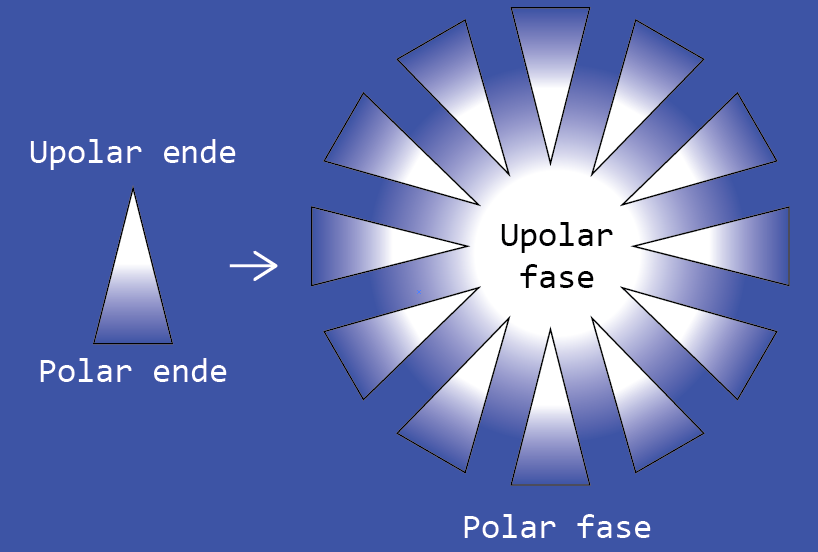
\includegraphics[width=0.8\linewidth]{micelle.png}
	\caption{Skjematisk illustrasjon av en surfaktant med et bredt polart hode og en smal upolar hale (typisk en ikke-forgrenet karbonkjede) som gir opphav til en micelle, som kan transportere dråper av olje i vannløsning.}
	\label{fig:micelle}
\emd\end{figure}

\paragraph{Reverserte miceller} Hvis surfaktanten består av et smalt polart hode og en bred upolar hale, så vil det dannes \emph{reverserte miceller}\index{reversert micelle} på samme måte som med miceller. Disse vil kunne transportere vann rundt omkring i en oljeløsning, som vist i Figur~\ref{fig:reversemicelle}. En egenskap ved reverserte miceller som man ikke observerer i miceller, er at reverserte miceller kan kollapse til én stor micelle, utveksle innhold, og så dele seg til to reverserte miceller igjen. En andre egenskap som er unik for reverserte miceller, er at størrelsen deres øker lineært med andelen vann i systemet; diameteren øker fra \SI{4}{\nano\meter} til \SI{18}{\nano\meter} når vannmengden $w=[\ce{H2O}]/[\ce{surfaktant}]$ øker fra $2$ til $20$.
\begin{figure}[H]
	\bmd\centering
	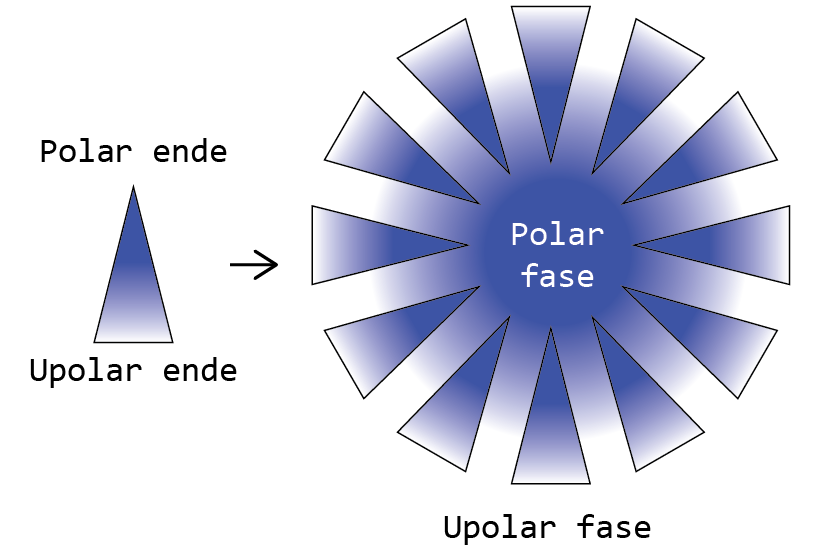
\includegraphics[width=0.8\linewidth]{reversemicelle.png}
	\caption{Skjematisk illustrasjon av en surfaktant med et smalt polart hode og en bred upolar hale (typisk en forgrenet karbonkjede) som gir opphav til en reversert micelle, som kan transportere dråper av et polart stoff i et upolart miljø.}
	\label{fig:reversemicelle}
\emd\end{figure}

\paragraph{Andre strukturer}
\begin{itemize}
	\item Dersom man har riktig mye vann i en oljerik løsning med surfaktanter, vil man i stedet observere at surfaktantene danner kanaler slik at man har alternerende regioner med olje og vann.
	\item Enda mer vann vil føre til at surfaktantene danner plane filmer (såkalt lamellær fase) som gjør systemet \idx{birefringent}, det vil si at det bryter lys forskjellig i forskjellige retninger.
	\item En siste mulig konfigurasjon av surfaktantene er såkalte \idx{superaggregat}er der surfaktantfilmen krummer seg innover og danner lag på lag med kulerunde strukturer (og sammenkoblede kanaler både på innsiden og utsiden av superaggregatet). Alle disse forskjellige strukturene kan (visstnok) forklares ut i fra geometrien til surfaktantmolekylene.
\end{itemize}

\paragraph{Reverserte miceller som nanoreaktorer} Egenskapen reverserte miceller har til å utveksle innhold kan brukes til å lage nanostrukturerte materialer med en helt bestemt størrelse på partiklene. Prosessen, slik den er beskrevet i Figur 18.9 i Bréchnigac et. al., gjengis her på norsk:
\begin{enumerate}
	\item Vi begynner med to separate løsninger med reverserte miceller. I den ene løsningen inneholder de reverserte micellene reaktant \ce{A}, i den andre inneholder de reaktant \ce{B}.
	\item Løsningene blandes. De reverserte micellene utveksler materiale.
	\item \ce{A} og \ce{B} reagerer inni cellene og danner produktet \ce{AB}. Reaksjonen er begrenset av størrelsen på micellene, så produktet vil være i form av nanopartikler og kan dermed ha forskjellige egenskaper fra bulk-materialet. Siden størrelsen på de reverserte micellene avhenger av vanninholdet, kan nanopartiklenes størrelse justeres ved å justere vanninnholdet.
	\item Micellene med produkt ekstraheres fra løsningen.
\end{enumerate}
Hvis vi bare hadde reagert \ce{A} og \ce{B} uten denne prosessen, ville vi fått produktet i form av bulkmaterialet. 


\setcounter{section}{19}
\ctitle{Elektrostatikk}
\paragraph{Dette kapittelet}
For å ta hensyn til elektriske interaksjoner i termodynamiske modeller, kan Coulombs lov brukes til å utlede et generelt uttrykk for elektrostatisk potensiell energi. Gyldighetsområdet til enkle modeller begrenses av at elektriske interaksjoner har lang rekkevidde.

\cstitle{Introduksjon til elektrostatikk}
Dette kapittelet følger forelesningene, som har en litt annen vinkling enn boka. Det meste bør være kjent fra et kurs i elektromagnetisme. Det er en kort introduksjon til elektrostatikk som begynner med Coulombs lov, og ender opp med et generelt uttrykk for elektrostatisk potensiell energi. Denne energien kan legges til den indre energien $U$, slik at vi kan ta hensyn til elektriske interaksjoner i det termodynamiske rammeverket vi har bygget opp i de tidligere kapitlene. 

\paragraph{Elektrostatisk potensiell energi} 
Den elektrostatiske potensielle energien $V$ mellom to punktladninger $q_i$ og $q_j$ med en innbyrdes avstand $R_{i,j}$ er gitt ved \i{Coulombs lov},
\begin{equation}
	V(q_i,q_j,R_{i,j}) = \frac{q_iq_j}{4\pi\epsilon_0R_{i,j}}
\end{equation}
der $\epsilon_0$ er permittiviteten til fritt rom, som er en universell konstant. Ofte ser man Coulombs lov i form av en kraftlov, men denne er helt ekvivalent. Hvis vi ser på interaksjonen mellom en testladning $q_t$ og en mengde ladninger $q_i$, og ser bort ifra innbyrdes elektriske interaksjoner (ladningene kan for eksempel være elektronene i et molekyl), får vi:
\begin{equation}
	V_t=\sum_{i=1}^N\frac{q_iq_t}{4\pi\epsilon_0R_{i,t}}
\end{equation}
Vi definerer \i{elektrostatisk potensial} $\psi_i$, ved ladning $q_i$, ved at $\psi_i$ må oppfylle
\begin{equation}
	\label{elpot}
	V_t=\sum_{i=1}^Nq_i\psi_i
\end{equation}
altså er
\begin{equation}
	\psi_i=\frac{q_t}{4\pi\epsilon_0R_{i,t}}
\end{equation}
Vi kan også snu på det og skrive
\begin{equation}
	V_t=q_t\psi_t
\end{equation}
der vi får fra definisjonen \eqref{elpot} at
\begin{equation}
	\psi_t=\sum_{i=1}^N\frac{q_i}{4\pi\epsilon_0R_{i,t}}
\end{equation}
\paragraph{Multipol-ekspansjon} Potensialet kan også uttrykkes som en Taylorrekkeutvidelse rundt et vilkårlig sentrum for molekylet. I én dimensjon blir det
\begin{equation}
	\label{psitaylor}
	\psi_i=\psi_i\rvert_{x=0}+r_{i,x}\frac{\partial \psi_i}{\partial x}\rvert_{x=0}+...
\end{equation}
Dette kan fint generaliseres til flere dimensjoner, men gjøres ikke her. Vi putter \eqref{psitaylor} inn i \eqref{elpot} og får at
\begin{align}
	V&=\sum_{i=1}^Nq_i\psi_i=\sum_{i=1}^N q_i\left(\psi_i\rvert_{x=0}+r_{i,x}\frac{\partial \psi_i}{\partial x}\rvert_{x=0}+...\right) \\
	&=\left(\sum_{i=1}^Nq_i\right)\psi_i\rvert_{x=0}+\left(\sum_{i=1}^Nq_ir_{i,x}\right)\frac{\partial \psi_i}{\partial x}\rvert_{x=0}+...
\end{align}
Hver av summene i rekka er et elektromagnetisk \emph{moment}. Vi definerer \i{molekylær ladning} eller (vi kunne også kalt det monopolmoment) $q_{\text{mol}}$ som
\begin{equation}
	q_{\text{mol}}=\sum_{i=1}^N q_i
\end{equation}
og \i{molekylært dipolmoment} $\boldsymbol{\mu}_{mol}$ som
\begin{equation}
	\boldsymbol{\mu}_{mol} = \sum_{i=1}^N q_i\vec{r}_i
\end{equation}
I én dimensjon blir disse vektorene i uttrykket til skalarer: $\mu_{mol}$ og $r_i$. Vi kunne gått videre og definert kvadropolmoment og oktopolmoment, men det blir perifert - men det kan nevnes at CO$_2$-molekylet, som verken har molekylær ladning eller molekylært dipolmoment (på grunn av symmetri), \emph{har} et kvadropolmoment.

Det \emph{elektriske feltet} \index{Elektrisk felt} $\vec{E}$ ved sentrum av molekylet er 
\begin{equation}
	\label{enabla}
	\vec{E}=-\nabla\psi
\end{equation}
I en dimensjon er det elektriske feltet ved sentrum av molekylet dermed
\begin{equation}
	E\rvert_{x=0}=-\frac{\partial \psi}{\partial x}\rvert_{x=0}
\end{equation}
Det endelige uttrykket vårt for elektrostatisk potensiell energi er
\begin{equation}
	V=q_{mol}\psi\rvert_{x=0}-\boldsymbol{\mu}_{mol}\cdot\vec{E}\rvert_{x=0}+...
\end{equation}
Rekka approksimeres ofte med de første to eller tre leddene. Denne potensielle energien kan legges til den indre energien $U$ og brukes sammen med resten av det termodynamiske maskineriet.

\paragraph{Elektriske interaksjoner i medier} Elektriske interaksjoner er svakere i medier, siden mediet blir \emph{polarisert}. \index{Polarisering} Polariseringen innebærer flere fenomener som alle bidrar til å gjøre det elektriske feltet fra frie ladninger svakere:
\begin{itemize}
	\item I medier med dipoler, orienteres dipolene i motsatt retning av feltet fra de frie ladningene.
	\item Elektronene i molekylene polariseres (elektronisk polariserbarhet).
	\item Atomene i molekylene endrer sin posisjon i molekylet (vibrasjons\-polariserbarhet)
\end{itemize}
Denne effekten beskrives med en \i{dielektrisk konstant} $D$ (også kjent som en \i{relativ permittivitet} $\epsilon_r$). Den innebærer intet mer enn en liten modifikasjon av Coulombs lov:
\begin{equation}
	V(r)=\frac{q_iq_j}{4\pi\epsilon_0DR}
\end{equation}
Noen verdier for $D$ er ca. 1 for luft, ca. 2 for hydrokarboner og proteiner, og ca. 78 for vann.

\cstitle{Begrensninger med nærmeste-nabo-modeller}
Elektriske interaksjoner har en ganske lang rekkevidde. Siden $V\propto 1/r$ vil også andre og tredje nærmeste nabo ha en innvirkning på $V$ fordi $1/r$ ikke har blitt tilstrekkelig liten til at vi kan se bort i fra den. Det er derfor ikke tilstrekkelig med gittermodeller som kun tar hensyn til nærmeste nabo, som vi har gjort tidligere. Et godt mål på hvor mange naboer vi trenger å ta hensyn til er gitt ved \i{Bjerrum-lengden} $l_B$, som er avstanden der den elektrostatiske potensielle energien er den samme som den termiske energien $RT$:
\begin{equation}
	RT=\frac{q_iq_j}{4\pi\epsilon_0Dl_B}
\end{equation}
dvs.:
\begin{equation}
	l_B=\frac{q_iq_j}{4\pi\epsilon_0DRT}
\end{equation}
Noen vanlige verdier er 56nm i luft og 0.7nm i vann. 

\cstitle{Elektrostatiske krefter}
Kraften $\vec{f}$ mellom ladninger er gitt som gradienten av det elektrostatiske potensialet:
\begin{equation}
	\vec{f}=-\nabla\frac{q_iq_j}{4\pi\epsilon_0DR}=\frac{q_iq_j}{4\pi\epsilon_0Dr^3}\vec{r}
\end{equation}
I tillegg har vi at Coulombs lov er additiv:
\begin{equation}
	V_{tot}=\frac{1}{2}\sum_{i}\sum_{j\neq i}\frac{q_iq_j}{4\pi\epsilon_0Dr_{ij}}
\end{equation}
der vi deler på to fordi vi summerer over hvert par to ganger.

Kraften fra en ladning $q$ på en testladning med størrelse lik enheten vi bruker ($q_{test}=1$) defineres som det $elektrostatiske feltet$:
\begin{equation}
	\vec{E}(\vec{r})=\frac{q}{4\pi\epsilon_Dr^3}\vec{r}
\end{equation}

\cstitle{Elektrisk fluks}
\i{Elektrisk fluks} $\Phi$ gjennom en flate $S$ er definert som
\begin{equation}
	\Phi=\int_S D\vec{E}\cdot\dS
\end{equation}
Et nyttig uttrykk for fluksen ut av en kuleflate med en punktladning $q$ i sentrum, er
\begin{equation}
	\Phi=DE(r)\int_SdS=DE(r)4\pi r^2=\frac{q}{\epsilon_0}
\end{equation}
\i{Gauss' lov} er at dette forholdet gjelder for \emph{alle} lukkede flater:
\begin{equation}
	\Phi=\frac{1}{\epsilon_0}\sum_{i=1}^n q_i
\end{equation}
eller, hvis vi har en ladningsfordeling (med ladningstetthet $\rho(\vec{r})$):
\begin{equation}
	\Phi=\frac{1}{\epsilon_0}\int_V \rho(\vec{r})\dv
\end{equation}


%!TEX root = Nanomat.tex
\ctitletwo{Cushing: Produksjon av nanopartikler med kjemiske metoder}
\addcontentsline{toc}{section}{CUSHING - PRODUKSJON AV NANOPARTIKLER MED KJEMISKE METODER}
\cstitletwo{Solvotermisk prosessering}
\paragraph{Autoklave} En autoklave er rett og slett en forseglet boks. En typisk autoklave består av en container av polytetrafluoroetylen (teflon) omsluttet av et tykt stålskall, med et tykt skrulokk av stål som er boltet fast med stålskruer. Her er en figur som beskriver alt du egentlig trenger å vite om en autoklave:
\begin{figure}[H]
	\centering
	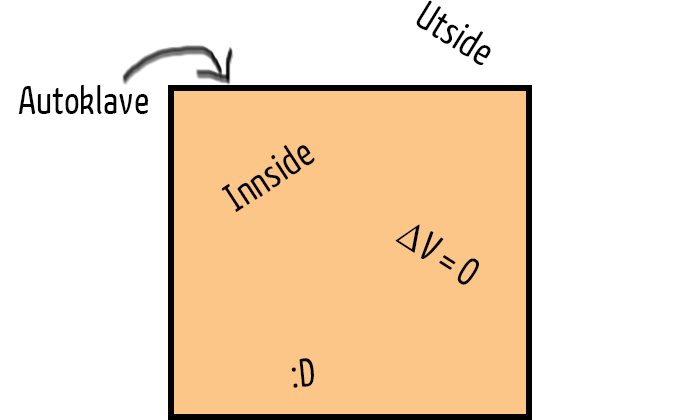
\includegraphics[width=0.95\linewidth]{autoklave.png}
	\label{fig:autoklave}
\end{figure}
Til våre formål er en autoklave den beste fysiske tilnærmingen til et lukket system:  volum og masse holdes konstant, mens temperatur kan kontrolleres utenfra. Autoklaver gjør det mulig å oppnå høyt trykk ved å øke temperaturen. Dette høye trykket gjør det mulig å utføre reaksjoner ved lavere temperaturer enn man ellers ville trengt.

\paragraph{Solvotermisk prosessering} er kjemiske prosesser som utføres i en lukket beholder (for eksempel en autoklave), slik at økt temperatur også medfører økt trykk.\footnote{Siden $pV=nRT$ og sånn. Altså, $pV$ er overhodet ikke lik $nRT$ i de fleste syntesene som beskrives her, siden vi ser på crazy blandinger av superkritiske fluider, surfaktanter, fast stoff og alt mulig rart, egentlig alt annet enn ideelle gasser. Uansett: det stemmer fortsatt at hvis $\Delta p > 0$ så er også $\Delta T > 0$.} Dette er betingelser som gir de oppløste stoffene \emph{økt løselighet og økt reaktivitet}.

Noen ganger økes trykk og temperatur såpass at man får et superkritisk løsemiddel, men ofte trenger man ikke å føre løsemiddelet forbi det kritiske punktet for å oppnå det man ønsker.

Slik bruk av en autoklave har flere fordeler:
\begin{itemize}
	\item Løselighet øker med trykk, så det høye trykket i en autoklave gjør at man oppnår en løselighet som man ellers ville trengt en langt høyere temperatur for å oppnå. Dermed kan man syntetisere materialer som ville blitt ustabile ved høye temperaturer.
	\item Reaksjonsproduktene er ofte krystalline, og trenger ikke den samme etterbehandlingen som man trenger ved bruk av kopresipitering eller sol-gel-metoder (som vi kommer til i de neste delkapitlene).
	\item En lukket beholder er et miljø der man presist kan kontrollere betingelser som pH og konsentrasjon av reaktanter.
\end{itemize}

For å utdype det siste punktet: her er en oversikt over hvordan forskjellige betingelser påvirker det endelige produktet. Det er dessverre få forklaringer på \emph{hvorfor} det er slik, men det finner man altså heller ikke mye av i Cushing.
\begin{itemize}
	\item Høy temperatur gir en bred fordeling av partikkelstørrelser. Lav temperatur gir en smal fordeling av partikkelstørrelser.
	\item Mineraliserende stoffer fører til redusert gjennomsnittlig partikkelstørrelse. De brukes også fordi de hjelper med å stabilisere forløperne og mellomproduktene i reaksjonen. Samtidig fører de også til agglomerering. Typiske mineraliserende stoffer er hydroksider, karbonater og halider.
	\item Aminer fungerer som ``capping agents'', som hindrer partikler fra å vokse forbi en viss maksimumstørrelse. Slike ``capping agents'' kan også forhindre agglomerering.
	\item Partikler vokser i størrelse over tid,\footnote{Hvis det var noen tvil.} så man kan kontrollere størrelsen ved å kontrollere tiden.
	\item Høy konsentrasjon av forløper gir høy faserenhet. Lav konsentrasjon fører til blandede faser.
	\item Krystallstrukturen til partiklene påvirkes av pH.
\end{itemize}

\paragraph{Hydrotermisk prosessering} er et spesialtilfelle av solvotermisk syntese der løsemiddelet er vann.

\paragraph{Mikrobølgeassistert solvotermisk prosessering} Man kan bruke mikrobølger til å forårsake veldig rask oppvarming av reaksjonsblandingen -- særlig hvis den inneholder vann. Dette gjør at partikler presipiterer raskt og nesten samtidig, som igjen gjør at partiklene blir veldig små, og har en smal størrelsesfordeling. Dette er en metode som brukes for å lage oksider og zeolitter (som vi skal snakke om i neste kapittel).

% Eks hydrot. syntese av kvarts: NaOH for å solubilisere silica ved lave T

% Autoklaver - gir kontrllert
% pH (kontrollere krystallstruktur)
% T (kontrollere dispersitet)
% t eller addisjon av surfaktaner/ioner (kontrollere størrelse)
% c (høyere konsentrasjon gir høyere phase purity)

% Continuous flow hydrothermal reactor
% X: mixing point: Ce-precursor, Zr-precursor, H20 near critical point
% PH: pre-heater, C: cooler, F filter

% Microwave-assisted solvothermal processing: what?

\paragraph{Presipitering og kopresipitering} Presipitering (eller utfelling) er dannelsen av fast stoff i løsning under en kjemisk reaksjon, typisk fordi reaksjonsproduktet har lavere løselighet i løsemiddelet enn reaktantene har. Kopresipitering er år flere forskjellige kjemiske specier presipiterer samtidig, og så danner mer komplekse systemer. Et eksempel på kopresipitering er når to forskjellige metaller presipiterer i samme løsning samtidig.

\paragraph{Egenskaper til utfellingsreaksjoner} Den vanligste måten å forårsake utfelling på, er kjemiske reaksjoner der produktet har lav løselighet i løsningen, slik at løsningen raskt blir overmettet. I slike reaksjoner er nukleering det viktigste trinnet. Sekundære effekter som Oswald ripening og agglomegering kan ha stor effekt på det endelige produktet. Reaksjonsbetingelser (for eksempel hvor raskt man legger til reaktanter, eller hvor raskt man rører i løsningen) kan naturligvis også påvirke det endelige resultatet.

\paragraph{Dispersjon} En dispersjon er et system der en kjemisk forbindelse er dispergert (det vil si at den finnes i form av finfordelte partikler) i en fase med en annen kjemisk sammensetning. Eksempler på dispersjoner er
\begin{itemize}
	\item Suspensjon, en dispersjon av partikler av fast stoff i væske.
	\item Sol, en dispersjon av kolloidale partikler av fast stoff i væske. Altså en suspensjon der partiklene er kolloider.
	\item Emulsjon, en dispersjon av væske (i veldig små dråper) i en annen væske.
\end{itemize}

\paragraph{Reduksjon av metall i løsning} En vanlig metode for å lage metall-nanopartikler er å \emph{redusere metalliske salter}. For å redusere et metallisk salt kreves det at endringen i fri energi er negativ. Dersom vi har standardbetingelser vil det si at cellepotensialet fra elektrokjemien, altså
\begin{equation}
	E^o_{\text{celle}} = E^o_{\text{reduksjon}} + E^o_{\text{oksidasjon}}
\end{equation}
skal være \emph{positivt}. Som regel har vi \emph{ikke} standardbetingelser, og må erstatte halvcellepotensialene i ligningen over med
\begin{equation}
	E = E^o - \frac{RT}{nF}\ln Q.
\end{equation}
Men dette er vi jo kjent med fra kjemi.

En metode for å sørge for at endringen i fri energi er negativ, er å bruke reduksjonsmidler. Noen vanlige reduksjonsmidler \emph{i vandig løsning} er:
\begin{itemize}
	\item Hydrogengass
	\item Solvaterte borohydridsalter, altså \ce{ABH4}, der \ce{A} er et alkalimetall
	\item Hydrasinhydrat \ce{N2H4.H2O} eller hydrasindihydro\-klorid \ce{N2H4.2HCl}\hfill
	\item Aminer
	\item Karboksylsyrer
	\item Alkoholer
\end{itemize}
Vann er ikke alltid egnet som løsemiddel. Hvis metallet er langt nede i spenningsrekka, altså edelt, kan man ikke bruke vann som løsemiddel.  Et reduksjonsmiddel som er kraftig nok til å redusere kationer fra et edelt metall, vil også være sterkt nok til å redusere vann i reaksjonen \ce{2H2O+2e- <-> H2+2OH-}, som har en $E^o=\SI{-0.8277}{\volt}$. Da må vi bruke ikke-vandige løsninger. Noen vanlige reduksjonsmidler \emph{i ikke-vandig løsning} er:
\begin{itemize}
 	\item \ce{NaBH4} og \ce{H2}, som før
 	\item DMF (N,N-dimetylformamid)
 	\item Alkoholer (særlig hvis vi har sterkt oksiderende kationer)
 	\item Alkalider, altså komplekser med alkalimetall-anioner som \ce{Na-}
 	\item Elektrider, altså komplekser med solvaterte elektroner (\ce{e- (aq)}, liksom). Solvaterte elektroner er det sterkeste reduksjonsmidlet som det er teoretisk mulig å lage.
 \end{itemize}
En annen grunn til å bruke ikke-vandige løsninger er at det ikke er alle produkter som er stabile i vandig løsning (eller mer generelt polare løsninger). For eksempel er kolloidale gullpartikler ikke stabile i polare løsninger. Men det kan fortsatt være gunstig å starte med en vandig løsning. Her er et eksempel på en prosess der man bruker både vandig og ikke-vandig løsning, for å lage kolloidale partikler av gull:
\begin{enumerate}
	\item Lag en vandig løsning med \ce{AuCl4-}
	\item Overfør \ce{AuCl4-} til en organisk fase ved å blande den vandige løsningen kraftig sammen med en løsning av tetraoktylammoniumbromid i toluen.
	\item Legg til dodekantiol i den organiske fasen. Dette er surfaktantene som blir sittende utenpå de kolloidale partiklene.
	\item Legg til en vandig løsning av \ce{NaBH4}. Dette blir redusjonsmiddelet. Rør kraftig.
	\item Det dannes kolloidalt gull med størrelse mellom 1 og 3 nm. La dette felles ut av løsningen.
	\item Isoler produktet som et tørt pulver. Ved å tilføre et uploart løsemiddel (eller et svakt polart et, som toluen) kan du få tilbake en stabil løsning av kolloidale gullpartikler.
\end{enumerate}

\paragraph{Andre metoder for å redusere metall} Det finnes noen andre metoder:
\begin{itemize}
	\item \emph{Elektrokjemisk reduksjon}, der metallet reduseres på en katode gjennom elektrolyse. Her trenger man et stabiliserende stoff for å unngå at metallet bare deponerer som en film på katoden.
	\item \emph{Strålingsassistert reduksjon}, der man bruker ioniserende lys til å spalte stoffer og lage radikaler, solvaterte elektroner og lignende. Disse kan så redusere metallet.
\end{itemize}

\paragraph{Utfelling av oksider fra vandig løsning} For å lage nanopartikler av krystalline oksider (hydroksider, karbonater, bikarbonater, oksalater, o.l.) kan vi få metallkationer til å kopresipitere, og så kalsinere dem. Det finnes to kategorier av reaksjoner som produserer oksider:
\begin{itemize}
	\item De som produserer et oksid direkte
	\item De som produserer en egnet forløper til et oksid. Forløperen må deretter prosesseres for å lage oksidet.
\end{itemize}
Det som er vanskelig ved utfelling av oksider er ikke å få til reaksjonen, men å få monodisperse partikler. Ved utfelling av oksider trenger man gjerne en stabilisator bundet til overflaten for å unngå aggregering. Med denne metoden kan man lage materialer som har funky støkiometriske formler (typ \ce{La_{$1-x$}Sr_$x$NbO4}), og kan fungere som
\begin{itemize}
	\item Protonledende elektrolytter
	\item Oksygenion-ledende elektrolytter
	\item Blandede ledere
	\item Anoder
	\item Katalysatorer
\end{itemize}

\paragraph{Utfelling av oksider fra ikke-vandig løsning} I vandig løsning bruker man ofte pH for å trigge utfelling. Hvis man trenger metaller som presipiterer ved veldig forskjellige pH må man bruke en ikke-vandig løsning. Ikke-vandige løsninger vil også forhindre prematur presipitering av hydroksider, som er vanlig i høyvalente kationer som \ce{Ti4+} og \ce{Zr4+}. Vanlige forløpere med denne metoden er tertiære metall-alkoksider, altså \ce{M(OR)4}. Dette er en bra metode for å lage bariumtitanat \ce{BaTiO3}. 

\cstitletwo{Sol-gel-prosessering}
Sol-gel er, kort forklart, \emph{hydrolyse og konsensering av metall-alkoksider}. Et metallalkoksid er noe som er på formen \ce{M(RO)_{$x$}}, altså en konjugerende base til et alkohol. Vi lager primært \emph{metalloksider} med denne metoden.

\paragraph{Aerogel!} Før vi går inn på metoden må det sies at det er sånn her man lager aerogel. Aerogel er et superluftig materiale som består av ultraporæst silisiumoksid. Det har et stort indre overflateareal og ekstremt lav varmeledningsevne. Det brukes derfor til varmeisolering, til tynnfilmer på selvrensende vinduer og til å samle støv fra kometer.

\paragraph{Metode} Sol-gel-syntese skjer i seks trinn:
\begin{enumerate}
	\item Dannelse av \emph{sol}, en løsning av metall-alkoksider eller metallkomplekser.
	\item Dannelse av \emph{gel}, et nettverk med oksid- eller alkohol-broer. Dette skjer ved polykondensering eller polyforestring.
	\item \emph{Aldring} (synerese), som skjer når polykondensasjonen har nådd punktet der gel-en er en solid masse. Gel-nettverket trekker seg sammen og gjør veggene sterkere, og noe av løsemiddelet fjernes.
	\item \emph{Tørking}: vann og andre flyktige væsker fjernes
	\item \emph{Dehydrering}: \ce{M-OH}-grupper på overflaten fjernes. Dette hindrer gel-en fra å rehydrere. Skjer ved ca. \SI{800}{\celsius}.
	\item Det siste trinnet skjer kun hvis man skal lage en xerogel for å lagge tette keramer eller glass. nemlig \emph{densification} der temperaturen er høyere enn \SI{800}{\celsius}. Porene i gel-nettverket kollapser, organiske specier fjernes.
\end{enumerate}
De første to trinnene bestemmer komposisjonen til det endelige materialet. 

\paragraph{Kjemiske reaksjoner i sol-gel-syntese} Det er to viktige reaksjoner som skjer i sol-gel-syntese:\footnote{Denne forklaringen av sol-gel-kjemi er ikke særlig bra. Beklager.}
I \emph{hydrolyse}trinnet erstatter man en \ce{OR}-gruppe med en \ce{OH}-gruppe ved å legge til vann i løsningen. Hydrolyse kan skje enten i sur eller i basisk løsning - det vil være enten \ce{H+}-ioner eller \ce{OH-}-ioner som katalyserer reaksjonen. Hydrolyse skjer saktere i sur løsning enn i basisk løsning. Antall \ce{OR}-grupper som hydrolyseres på alkoksidet kalles \emph{hydrolyseringsgraden}, og denne avhenger av forholdet mellom metall-forløper og vann. Mye vann fører til høyere hydrolyseringsrad. For eksempel, for TEOS (tetraetylortosilikat):
\begin{equation}
	\ce{ Si(OR)4 + nH2O -> Si(OR){4-n}(OH)n+nROH }
\end{equation}
Under \emph{kondensering}strinnet dannes det en polymer gjennom polykondensasjon. Kondensasjonsreaksjonen kan enten være \emph{alkoksalering} eller \emph{oksalering}. Veldig forenklet kan man si at alkoksalering er når det lages en binding mellom \ce{OR}-gruppen til ett metall-alkoksid og \ce{OH}-gruppen til et annet metall-alkoksid samtidig som man spalter av en \ce{ROH} --- mens oksalering er når det lages en binding  \ce{OH}-gruppene til to metall-alkoksider samtidig som man spalter av en \ce{H2O}. Oksalering er mye raskere fordi \ce{OH}-gruppen er en bedre utgående gruppe enn \ce{OR}.

Hydrolyseringsgraden $n$ bestemmer hva slags produkt man får. Når $n=1$ får man dimerer, hvis $n=2$ får man 1-dimensjonale kjeder eller 2-dimensjonale ringer, og hvis $n=4$ får man 3-dimensjonale nettverk og fraktaler. 

\paragraph{Effekten til pH} Årsaken til at pH har noe å si for strukturen det endelige produktet, er at \emph{hydrolysen skjer raskere i basisk løsning}. Når hydrolysen skjer raskt, vil det tidlig dannes mange hydrolyserte grupper som kan kondensere. Dette gjør at det tidlig dannes forgreinede molekyler og klynger som lager tette nettverk på liten skala. Etter hvert som kondensasjonen fortsetter, vil strukturen vokse ved at forskjellige klynger går sammen, så man får et nettverk av klynger.

I sur løsning skjer hydrolysen tregere. Dette gjør at de kondenserte molekylene er mer lineære tidlig i prosessen. Det er først senere i prosessen at de møter hverandre og danner et sammenvevd nettverk. 

\paragraph{Endelige produkter} Det finnes tre typer endelige gels, som klassifiseres etter styrken av det inorganiske nettverket:
\begin{itemize}
	\item I en \emph{xerogel} er nettverket svakt, og det kollapser under tørking. Dette skjer når løsemiddelet har høy overflatespenning, slik at det ``drar'' på gel-nettverket (i form av kapillærkrefter) når det tørker.
	\item I en \emph{ambigel} har man en mellomting mellom en xerogel og en ambigel. Dette får man når løsemiddelet har lav overflatespenning, slik at løsemiddelet ikke drar så mye på nettverket under tørking.
	\item I en \emph{aerogel} er nettverket sterkt, og beholder nettverksstrukturen under tørking. Dette kan man få ved å bruke et superkritisk fluid som løsemiddel, da et superkritisk fluid ikke har overflatespenning.
\end{itemize}
Gel-en kan være det endelige produktet, eller det kan være en forløper som kalsineres eller sintres for å lage produkter som tette nanokrystalline keramer eller tette filmer.

De vanligste produktene i sol-gel-syntese er oksider, men man kan også lage ting som karbider, nitrider og sulfider. I så fall må man unngå hydrolysen da dette per definisjon gir oksider. Da bør man bruke et aprotisk, inert løsemiddel i stedet for vann.

%Produksjon av komposittmaterialer:  % Eksempler: kvanteprikker i silicatynnfilm
%\begin{enumerate}
%	\item 
%	\item 
%	\item 
%\end{enumerate}

\paragraph{Pechini-metoden} er en alternativ sol-gel-prosess for metaller som ikke lar seg hydrolysere så lett, for eksempel alkalimetaller, jordalkalimetaller og overgangsmetaller.\footnote{Så... egentlig alt unntatt aluminium, gallium, indium, selen, titan, bly og vismut.} Med Pechini-metoden bruker man organiske ting som sitronsyre, som lager komplekser med disse metallene. Man legger også til et polyaklohol som glykol. Gel-en dannes i dette tilfellet gjennom en polyforestring der sitronsyre og glykol inngår, mens metallet bare slenger seg på sitronsyra. Etter at man har tørket gel-en kan man varme det opp for å bryte ned det organiske stoffet og få et agglomerat av oksidpartikler.

Problemet med denne metoden er at det er vanskelig å kontrollere størrelse, form og morfologi, og at man stort sett får sfærise partikler. Derfor brukes denne metoden først og fremst for å lage fine partikler som deretter kan sintres for å danne tette keramer. Sintring kommer vi til i kapittel 21.

Denne metoden brukes for å lage \ce{BaTiO3}.

\setcounter{section}{10}
%!TEX root = Nanomat.tex
\ctitle{(og 26) Nanoporøse stoffer}
Nå som vi har sett på superkritiske fluider og hydrotermisk syntese\footnote{Kremt.} er vi klare for å se på noen produkter som kan lages med denne syntesen, nemlig stoffer med bittesmå porer.

\paragraph{Terminologi for nanoporøse stoffer} Et nanoporøst stoff består av et uorganisk ``skjelett'', som regel negativt ladet, som inneholder hulrom eller tuneller. Den negative ladningen til skjellettet balanseres av uorganiske kationer eller vannmolekyler rundt om kring. Terminologien rundt nanoporøse materialer er litt pussig:
\begin{itemize}
	\item \emph{Mikroporøse} materialer har porer med en diameter som er mindre enn \SI{2}{\nano\meter}.
	\item \emph{Mesoporøse} materialer har porer med en diameter mellom \SI{2}{\nano\meter} og \SI{50}{\nano\meter}.
	\item \emph{Makroporøse} materialer har porer med en diameter som er større enn \SI{50}{\nano\meter}.
	\item Alle de ovennevnte tilhører det vi klassifiserer som \emph{nanoporøse} materialer. What?
\end{itemize}

\cstitle{Uordnede nanoporøse stoffer}
Dette er nanoporøse stoffer som ikke har en noen periodisk struktur (over store avstander). Disse kan lages industrielt på en av to måter:
\begin{itemize}
	\item Aggregering og delvis sintring av partikler\footnote{Se kapittel 21 om sintring.}. Her vil porene være hulrommene som gjenstår mellom partiklene. Aggregering og delvis sintring danner hovedsakelig mesoporøse og makroporøse materialer. Jo mindre de opprinnelige partiklene er, jo større vil det spesifikke overflatearealet til produktet bli. Silica-gel og porøse keramer er to eksempler på porøse stoffer som kan lages med en slik prosess.
	\item Materialer der man danner porer ved å selektivt løse opp deler av et opprinnelig ikke-porøst materiale. Et eksempel på et materiale laget med en slik prosess er Vycor, et porøst glass. Dette lages ved å varme opp \ce{Na2O-B2O3-SiO2}-glass (med en passende sammensetning av de tre komponentene) til \SI{1400}{\celsius}, og så kjøle ned til en temperatur mellom \SI{450}{\celsius} og \SI{700}{\celsius}. Hvis man gjør dette riktig, vil materialet separere i to faser gjennom såkalt \emph{spinodal dekomponering} i stedet for den vanlige mekanismen for faseseparasjon (nukleering og kornvekst). Ved spinodal dekomponering skjer faseseparasjonen spontant gjennom hele materialet slik at man får et materiale bestående av to sammenvevde nettverk. Det ene nettverket består av 96\% silica, det andre stort sett av natriumborat. Natriumborat er mer syreløselig enn silica, så etter syrebehandling står man igjen med rent silicaglass som har en ormelignende porestruktur. Størrelsen på porene kan justeres med temperaturen og varigheten til prosessen, samt syrestyrken.
\end{itemize}

\cstitle{Ordnede mikroporøse stoffer: zeolitter}
Av stoffer med periodisk struktur har vi mikroporøse \emph{zeolitter}, samt ordnede mesoporøse stoffer. 

\paragraph{Zeolitter} Zeolitter er et kort ord for krystallinske aluminosilikater. Zeolitter består av et porøst, negativt ladet, uorganisk skjelett av silisium, oksygen og aluminium, som balanseres av vannmolekyler og kationer fra alkali- og jordalkalimetaller som henger i porene. I skjelettet inngår hvert oksygenatom i to tetraedere - ett av dem med \ce{Al} i sentrum og det andre med \ce{Si} i sentrum, som man så vidt kan skimte i Figur~\ref{fig:faujasite}. Skjelettet har en periodisk struktur med hulrom eller kanaler som kan være fra \SI{0.3}{\nano\meter} til \SI{0.8}{\nano\meter} -- det finnes utallige typer zeolitter med forskjellig størrelse og sammensetning av hulrom og kanaler.
\begin{figure}[H]
	\bmd\centering
	\includegraphics[width=0.9\linewidth]{faujasite.png}
	\caption{Atommodell av zeolittarten faujasitt. \ce{Si} i grått, \ce{Al} i blått og \ce{O} i rødt.}
	\label{fig:faujasite}
\emd\end{figure}
Før i tida var begrepet ``zeolitt'' begrenset til \emph{naturlige} krystallinske aluminosilikater, men ordet har i dag en utvidet betydning. I dag kan det også referere til stoffer der noe av silisiumet er byttet ut med et annet grunnstoff. Dette grunnstoffet kan være et trivalent grunnstoff som \ce{Al}, \ce{Fe}, \ce{B} og \ce{Ga} eller et tetravalent grunnstoff som \ce{Ti} og \ce{Ge}.

\paragraph{Syntese av krystalline mikroporøse faste stoffer}
Krystalline mesoporøse faste stoffer lages ved hydrotermisk krystallisering av en gel som inneholder både en væskefase og en fast fase. Reaksjonsmediet inneholder
\begin{itemize}
	\item Kjemiske forløpere til rammeverket i strukturen, altså ting som \ce{Si}, \ce{Al} og/eller \ce{P}.
	\item Inorganiske kationer, og/eller organiske specier, som skal balansere den negative ladningen til rammeverket. De spiller også andre roller: de fyller opp mikroporene, de kan påvirke strukturene som dannes, de kan endre de kjemiske egenskapene til gel-en, og de kan stabilisere byggeblokkene i det inorganiske rammeverket.
	\item Kjemiske forløpere til de mineraliserende agentene, altså ting som produserer \ce{OH-} og/eller \ce{F-}. Disse skal balansere mellomtrinnene under sol-gel-prosessen.
	\item Et løsemiddel, typisk vann.
\end{itemize}

Prosessen innebærer at
\begin{itemize}
	\item Reaktantene blandes grundig.
	\item Blandingen holdes ved romtemperatur en stund (ripening).
	\item Blandingen puttes i en autoklave og varmes opp.
\end{itemize}

\paragraph{Syntese av zeolitter} For zeolitter er betingelsene slik:
\begin{itemize}
	\item Basisk medium.
	\item Temperatur på under \SI{200}{\celsius}.
	\item Relativt lavt trykk. Det autogene trykket i autoklaven er på under \SI{20}{\bar}
	\item Tiden det tar kan være alt fra noen timer til flere dager.
\end{itemize} 
Produktet man da får, må vaskes med destillert vann, filtreres og tørkes. Dette produktet er \emph{ikke} porøst, for porene er fylt opp med de inorganiske og/eller organiske kationene som man brukte til syntesen. Man må derfor etterbehandle produktet for å få tilbake porene. Dette kan innebære å bytte ut kationene med andre kationer som man heller vil ha der,\footnote{Ikke spør meg hvordan man gjør det.} eller ved å varme opp til sånn fem hundre grader sånn at eventuelle organiske stoffer brytes ned.\footnote{Tror jeg. Klarte ikke helt å dekryptere setningen ``Porosity is reinstated after cation exchange (inorganic cations) and/or calcination (ammonium cations and organic species)''.}

\paragraph{Bruksområder for zeolitter} Disse finnes det en del av:
\begin{itemize}
	\item Porene gir zeolitter et stort indre overflateareal, som kan gjøre zeolitter nyttige innen \emph{katalyse}; de brukes i olje- og gassindustrien for separasjon av gass.
	\item Det indre overflatearealet gjør også at zeolitter kan adsorbere mye materiale. Derfor brukes de til å adsorbere illeluktende stoffer som \ce{H2S} og formaldehyd.
	\item Den bestemte størrelsen til porene gjør at zeolitter kan brukes som molekylære siler, for eksempel for å filtrere ammonium.
	\item Porene kan fylles med gjødsel, som så slippes ut over lengre tid. Dette gjør det mulig å bruke gjødsel mer effektivt og med mindre avrenning. 
\end{itemize}

\cstitle{Ordnede mesoporøse stoffer}
\paragraph{Ordnede mesoporøse stoffer} Dette er en type silikater og aluminosilukater der porene fortsatt er veldefinerte og har en smal størrelsesfordeling, men nå er de litt større enn det man kan lage med zeolitter. 

Konkrete eksempler på ordnede mesoporøse stoffer er M41S-familien. Medlemmer av denne familien er MCM-41, som har porer ordnet i et (nesten) regulært heksagonalt gitter; MCM-48, som har kubisk symmetri; og MCM-50, som har lamellær struktur. MCM står for Mobile Composition of Matter, av en eller annen grunn.

\paragraph{Syntese av ordnede mesoporøse stoffer} Syntese av ordnede mesoporøse stoffer ligner veldig på prosessen for å syntetisere zeolitter. Denne typen syntese gjøres imidlertid ved litt lavere temperaturer, typ \SI{25}{\celsius} til \SI{150}{\celsius}. I reaksjonsmediet har man gjerne noen surfaktanter,\footnote{Kvartære ammoniumkationer på formen \ce{C_{$n$}H_{$2n+1$}(CH3)3N+}, hvis du lurte.} der den vanligste kalles CTAB\footnote{Heksadekyltrimetylammonium-bromid.} der lengden på alkylkjeden til surfaktanten bestemmer diameteren til kanalen. 

Det er ingen som egentlig vet hvordan disse mesoporøse stoffene faktisk dannes. Her er et forslag til hvordan det kan foregå:
\begin{enumerate}
	\item Surfaktanter danner sylindriske miceller.
	\item Micellene selvorganiserer seg til heksagonale eller kubiske gitre, eller til lamellære (ormelignende) strukturer, avhengig av prosessen.\footnote{Se kapittel 22 om selvorganisering. Det bør gi litt intuisjon om hva som skal til for å danne et heksagonalt gitter.}
	\item En keramisk forløper binder seg til surfaktanthodene, og ``kondenserer'' der som en keramisk fase på utsiden av micellestrukturen.
	\item Surfaktantene fjernes, slik at det som står igjen er den keramiske fasen med mesoporøs struktur.
\end{enumerate}

\paragraph{Bruksområder for ordnede mesoporøse stoffer} Ordnede mesoporøse stoffer er et nyttig substrat som man kan putte funksjonelle monolag på, for å lage funksjonelle mesoporøse materialer (de kan for eksempel fungere som væskefiltre og sånn).

\cstitle{Ordnede makroporøse stoffer}
Boka sier ingenting om ordnede makroporøse stoffer. Det er jo litt synd, for jeg har hørt at du kan lage stoffer med interessante optiske egenskaper (porestørrelsen begynner jo å nærme seg bølgelengden til synlig lys) og sånn.


%\setcounter{section}{25}
%%!TEX root = Nanomat.tex
\ctitle{Nanoporøse stoffer II - nanoporøse medier}




% No mineralizer!

% Tydeligvis MCM-41 som er kult

% C_{16}TMA - størrelsen på miceller bestemmer størrelsen på porene som dannes

% Vanskelig å finne ut av reaksjonsmekanismene - hva som faktisk skjer under reaksjonen. Det ble først foreslått at mesoporøs struktur kommer direkte fra micellestruktur, men nå tror vi på Frasch-modellen.

% Sylindriske miceller i heksagonale arrays: LCT = Liquid Crystal Templating. Figur viser to forskjellige måter å få til det samme på (legge til SiO2 før eller etter assembly)

% Betingelser for MCM-41-fase: se foil.

% 5-celt diagram: Huo-modellen. I trinn B/C er det ingen kondensering - ingen binding mellom de inorganiske speciene. Det skjer først i trinn D.

% Hva er det som gjør at man får enten B eller C? 
% B: lavt nivå av polykondensasjon og høy ladningstetthet. 
% C: motsatt
% Ladningsbalanse mellom surfaktanter og inorganiske specier spiller en rolle i den endelige strukturen.

% Frasch-modellen:. 
% A: initial cationic micelles. Note that there are some surfactants which do not belong to the micelle
% -> add the silica precursors
% B: Silica precursors form around the micelle. Small exchange of ions, but no formation of structure
% -> reduce the pH and add heat
% C: silica precursors precipitate to become silicious prepolymers that may bind to the free surfactants. 
% D: These prepolymers grow and form polymers that can bind more surfactants and eventually form complete  layers of silica around smaller micelles.
%
% Tabell: bare noen eksempler fra boka. 
%
% Må vite: struktur til zeolitter. Beskriv tetraederne (forrige forelesning) som danner byggestener for zeolitter. Vit at man alltid trenger kationer eller vann for å balansere nettverket. Beskriv kort syntesen. Mange applikasjoner som kan beskrives, de er overalt.
% Krystalline vegger vs. amorfe vegger, ordnede vs. uordnede stoffer. Standard karakteriseringsmetoder kommer *senere*.

















%!TEX root = Nanomat.tex
\ctitletwo{Xia - Endimensjonale nanostrukturer}
\addcontentsline{toc}{section}{XIA - ENDIMENSJONALE NANOSTRUKTURER}
Metodene vi skal se på i dette kapittelet er generelle metoder som er egnet for alle faste stoffer.

\cstitletwo{Template-directed synthesis}
\paragraph{Templat} I ``template-directed synthesis'' har man en templat (eller mal, om du vil) som er et skjelett eller en ramme for strukturen man kan lage. Strukturen man ender opp med vil dannes inni eller rundt templaten, så man vil få en struktur som er komplementær med formen til templaten. 

\paragraph{Fordeler med templater} Vi liker å bruke templater fordi
\begin{itemize}
	\item Det er en enkel metode
	\item Man kan lage strukturer med en veldig kompleks form i ett enkelt trinn
	\item Man kan lage mye om gangen
	\item Det er kostnadseffektivt
\end{itemize}

\paragraph{Ulemper med templater} Men det er noen problemer med templater:
\begin{itemize}
	\item Det er ofte nødvendig å fjerne templaten, og dette må gjøres selektivt (uten å også fjerne strukturen vi har laget). Dette kan gjøres med kjemisk etsing eller varmebehandling.
	\item Strukturene man lager er gjerne polykrystalline
	\item Man får ganske liten mengde per syntese man gjør % what? men high throughput?
\end{itemize}

\cstitletwo{Ting som kan brukes som templater} 
Noen eksempler på templater er:
\begin{itemize}
	\item Nanostrukturer som har blitt syntetisert med andre metoder
	\item Biologiske makromolekyler, for eksempel DNA-kjeder eller virus som har en nyttig form
	\item Selvorganiserte strukturer
	\item Kanalene i et poræst materiale
	\item Skarpe kanter på overflaten av et solid substrat
\end{itemize}
la oss se på hver av dem:

\paragraph{Detaljer på overflaten av et solid substrat} Hvis vi har et solid substrat med en en eller annen regulær struktur, kan vi bruke geometrien til å ``dekorere'' substratet med nye strukture. Se figur i Xia om dette...

\paragraph{Kanaler i porøse materialer} Vi kan enten fylle kanalene helt opp for å få solide rør, eller vi kan fylle dem delvis opp slik at materialet kun vil være på kantene av kanalene. De endelige produktene blir da hule rør. Det porøse materialet kan være
\begin{itemize}
	\item en polymerfilm som har blitt bestrålt med tunge ioner for å danne skader i filmen, som så utvides med kjemisk etsing. Dette danner uniforme, sylindriske porer gjennom filmen, som er spredt tilfeldig utover. Disse kan fjernes ved å bruke høy temperatur.
	\item aluminiumfolie som gjøres til en anode i et surt miljø. Dette danner tettpakkede (heksagonale) sylindriske porer med uniform størrelse. Denne templaten kan etses bort med \ce{NaOH}.
	\item mesoporøse materialer med kanaler på mellom \SI{1.5}{\nano\meter} og \SI{30}{\nano\meter}
\end{itemize}
Med denne metoden kan vi lage mye forskjellig: metaller, halvledere, keramer og organiske polymerer. Porene kan fylles med gassfase-sputring, injeksjon i væskefase eller elektrokjemisk deponering (se kapitlene om tynnfilmer).

\paragraph{Selvorganiserte molekylære strukturer} Vi kan også bruke strukturene som vi lagde i kapittel 18 om kolloider. Ved riktig konsentrasjon danner surfaktantmolekyler spontant rørformede miceller (eller inverse miceller). Med en passende kjemisk reaksjon kan vi fylle opp disse rørene med et annet materiale, og danne nanorør på den måten.

\paragraph{Eksisterende nanostrukturer} Hvis vi har klart å lage en nanostruktur, kan denne kanskje brukes som templat til syntese av nye, mer komplekse strukturer. For eksempel kan man dekke nanotråder med et nytt materiale for å få ``core-shell nanowires''. Hvis vi så fjerner den opprinnelige nanotråden, står vi igjen med et hult nanorør. Vi kan også kjemisk reagere strukturene -- dette har blitt gjort for å omdanne silisium-nanotråder til silisiumoksid-nanotråder (ved oppvarming og oksidering), og for å omdanne karbon-nanotråder til metallkarbid-nanotråder.

Bruk av eksisterende nanostrukturer er også en veldig nyttig metode for å lage nanotråder av et materiale som ikke gror nanotråder naturlig. Så i stedet for å gro nanotråder av materialet fra bunnen av, begynner man med å lage nanotråder av f.eks \ce{MgO} (som er lett å lage), og dekker så disse nanotrådene med materialet man er interessert i. Med denne metoden har man klart å lage kjempemagnetoresistente nanotråder av \ce{La_{0.67}Ca_{0.33}MnO3}.

\cstitletwo{Endimensjonal vekst}
Her skal vi se på metoder for å gro nanotråder ut av et isotropt medium. Metodene vi brukes kalles VS, VLS og SLS og står for henholdsvis ``vapor-solid'', ``vapor-liquid-solid'' og ``solution-liquid-solid''. De er ganske like, forskjellen ligger altså i hvilken fase reaktantene befinner seg i.

\paragraph{Grad av overmetting bestemmer form} Formen på strukturen vi ender opp med i disse metodene, har å gjøre med hvor overmettet løsningen (eller dampen) vi begynner med er:
\begin{itemize}
	\item Lav overmetting gir fibre og hårlignende strukturer.
	\item Medium overmetting gir vekst av bulk-krystallet.
	\item Høy overmetting gir pulver, som dannes ved homogen nukleering.
\end{itemize}

\paragraph{Vapor-solid (VS)} VS heter det det gjør fordi materialet man skal lage nanotråd av begynner i gassfase, og transporteres til substratet. Substratet holdes ved en relativt lav temperatur, slik at materialet kan kondensere og danne nanotråder der. VS kan skje på to måter:
\begin{itemize}
	\item Direkte: materialet man skal lage en nanotråd av, fordampes, før det transporteres til substratet. og kondenserer der.
	\item Indirekte: det dannes forløpere til materialet man skal lage en nanotråd av før det dannes nanotråder.
\end{itemize}
Man vet ikke alltid om metoden man bruker er direkte eller indirekte, fordi man ikke helt vet mekanismen for VS enda.

\paragraph{Vapor-liquid-solid (VLS)}
VLS-vekst er til nå den mest suksessfulle metoden for å lage store mengder av nanotråder med enkrystallin struktur. I denne metoden begynner man med nanostore dråper av katalysatormetall, som man løser opp gassreaktanter i. Hver av dråpene kommer til å korrespondere til én tråd i det endelige produktet. 

Forutsetningen for at dette skal fungere, er at katalysatormetallet kan danne en væske-legering med materialet man ønsker å lage nanotråder av. Den største utfordringen i VLS er altså å finne en katalysator som passer med nanotråd-materialet. %Ideelt sett skal man kunne danne en eutetisk blanding  (påminnelse: ved den eutetiske sammensetningen av en legering kommer hele legeringen til å smelte samtidig (ved en temperatur som kalles den eutetiske tempearturen), i stedet for at én fase smelter først og så den andre).

Mekanismen er enkel: dråpene med katalysatormetall og reaktanter sitter på overflaten av substratet. Det tilføres stadig mer reaktanter, så dråpene er alltid overmettet med reaktant. Dette gjør at reaktanten presipiterer i grenseflaten mellom dråpen og substratet. Presipiteringen fortsetter etter hvert som man tilfører mer reaktant, og man ender opp med at det gror en nanotråd mellom substratet og dråpen. Se fig. 15 A i Xia (det er sikkert også nyttig å prøve å forstå fasediagrammet i fig. 15 B).

Produkter som har blitt laget med VLS:
\begin{itemize}
	\item Elementære halvledere som \ce{Si} og \ce{G}
	\item III-V-halvledere som \ce{GaAs} og \ce{InP}
	\item II-VI-halvledere som \ce{ZnS} og \ce{CdSe}
	\item Binære oksider som \ce{ZnO} og \ce{SiO2}
\end{itemize}
Det er per i dag \emph{ikke} mulig å bruke VLS til å lage nanotråder av metaller og ternære oksider.

\paragraph{Solution-liquid-solid (SLS)}
SLS er som VLS, men som man kanskje skulle forutsi ut i fra navnet bruker man en løsning med forløpere i stedet for en damp. Av en eller annen grunn skal man da bruke metallorganiske forløpere (som dekomponerer til metall pluss organisk biprodukt), og katalysatoren skal være et metall med lavt smeltepunkt som indium, tinn eller vismut.

\paragraph{Bruk av ``capping reagents''} Hvis vi husker tilbake til kapittel 1, så er likevektsformen til en krystall den der overflateenergien er minimert, og dette skjer når det er et visst forhold mellom de forskjellige fasettene i krystallen (Wullfs teorem). Vi kan også se på det med kinetikk: krystallplanene med høyest overflateenergi er de mest reaktive og dermed de som vokser raskest. De krystallplanene som vokser raskest, vil forsvinne i den endelige stukturen, og gjør at de planene som gror sakte, ender opp med å bli fasettene i produktet.

Men hva om vi er interessert i en struktur der det er mer av de mest reaktive krystallplanene? For å endre likevektsstrukturen til krystallene (og dermed strukturen til produktet vårt) kan vi bruke molekyler som modifiserer overflateenergien til visse fasetter. Surfaktanter kan brukes til dette.

\cstitletwo{Andre metoder}
\paragraph{Selvorganisering av kolloidale nanopartikler} Vi kan bruke de selvorganiserende egenskapene til kolloidale nanopartikler (mer om dette i kapittel 22). Dette gjør vi ved å fylle en eller annen template med de kolloidale partiklene. Templaten kan for eksempel være basert på en struktur som vi har mønstret på forhånd. Vi kan også manipulere organiseringen av partiklene med prober, eller ved å påføre elektriske eller magnetiske felt.

\paragraph{Metoder for å redusere størrelsen på 1D-strukturer} Hvis vi har strukturer med en bredde i størrelsesorden 1 til 10 \si{\micro\meter}, og ønsker å redusere størrelsen til ca. 100\si{\nano\meter} eller mindre, finnes det noen forskjellige metoder:
\begin{itemize}
	\item Strekk tråden i lengderetningen. Da blir den lengre og tynnere. Dette krever selvfølgelig at man har et materiale som er mykt nok til å strekkes på denne måten, men man har fått det til med metaller og glass som har blitt varmet opp til litt under smeltepunktet.
	\item Anisotrop etsing av en enkrystall (hm...)
	\item Bruk litografi
\end{itemize}

\cstitletwo{Egenskaper og bruksområder for 1D-nanostrukturer}
\paragraph{Egenskaper for 1D-nanostrukturer} Noen ting som er godt å vite om 1D-nanostrukturer er:
\begin{itemize}
	\item Jo mindre diameteren på nanotråden er, jo lavere smeltepunkt har den (akkurat som at smeltepunktet synker med minkende størrelse for nanopartikler). Når smeltepunktet blir lavere, er det lettere å gjøre varmebehandling for å få defektfrie nanotråder. Det blir lettere å kutte og sveise sammen nanotråder ved temperaturer som ikke skader materialet. Men det lave smeltepunktet kan også bli et problem, fordi det kan hende at nanotrådene brytes opp til kortere segmenter (de kortere segmentene har lavere fri energi, og når smeltepunktet er lavt skal det ikke så mye til for å overkomme energibarrieren det innebærer å bryte opp nanotråden).
	\item Énkrystalline nanotråder har færre defekter per enhet lengde. Siden defekter gjerne er det som fører til mekaniske feil, bør enkrystalline nanotråder være langt sterkere enn bulkmaterialet.
	\item Enkelte metall-nanotråder kan ende opp med å bli til halvledere dersom diameteren blir liten nok.
\end{itemize}

\paragraph{Bruksområder for 1D-nanostrukturer} Disse strukturene er særlig nyttige for å lage presise sensorer. De har ekstremt høyt forhold mellom overflate og volum, og dette gjør at de elektroniske egenskapene til nanotrådene blir ekstremt sensitive til molekyler som adsorberes på overflaten av nanotrådene. 

Et eksempel på dette er nanotråder av enkrystallint tinndioksid (\ce{SnO2})\footnote{Litt bedre forklaring enn den i Xia finnes her: http://nanowires.berkeley.edu/wp-content/uploads/2013/01/058.pdf}.  Enkrystallint \ce{SnO2} er en n-type halvleder med elektrisk ledningsevne som avhenger sterkt av overflatetilstanden, som igjen er påvirket av molekyler som adsorberes på overflaten. Det har seg slik at molekyler av forurensningsgassen \ce{NO2} fanger opp elektroner dersom de adsorberes på overflaten. En annen egenskap ved \ce{SnO2}-nanotråder som vi tar i bruk er at deres elektriske egenskaper er svært sensitive for UV-lys: UV-lys med bølgelengde på \SI{254}{\nano\meter}, har fotonene en del høyere energi enn båndgapet til \ce{SnO2}, så hvis man bruker slikt lys på nanotrådene øker ledningsevnen med 3-4 størrelsesordener. UV-lys gjør også at \ce{NO2} kan desorbere fra nanotråden (hvis vi ikke bruker UV-lys, vil ikke \ce{NO2} forsvinne når de først har satt seg på nanotråden). Dermed kan vi bruke \ce{SnO2}-nanotråder pluss UV-lys til å måle \ce{NO2}. Det som er fint er at vi kan gjøre det ved romtemperatur, mens vi måtte påført temperaturer på minst \SI{300}{\celsius} hvis vi skulle brukt \ce{SnO2} i form av pulver eller tynnfilmer -- ikke særlig gunstig når vi har å gjøre med en gass som ofte dannes i ekspolosive prosesser.

Halvleder-nanotråder finnes også, og de kan kanskje brukes til noe nyttig en dag. Blant annet er det snakk om å lage enkelt-foton-kilder.



%* Nanotråder av III-V-halvledere ved lavere temperaturer
%* Superkritisk fluid som løsemiddel
%* En viktig komponent er den molekylere komponenten hvis konstituerende grupper kan elimineres for å generere en ikke-molekylær enhet som man kan sette sammen nanotråder av

%!TEX root = Nanomat.tex
\ctitletwo{NS1 Litografi og etseprosesser}
\cstitletwo{Litografiteknikker}
I denne sammenhengen betyr litografi at man lager et mønster i en tynnfilm som kalles en resist. Vi kategoriserer litografiteknikker etter hva slags interaksjon som brukes for å modifisere resisten:
\begin{itemize}
	\item I fotolitografi bestråler man resisten med lys.
	\item I elektronlitografi bestråler man resisten med elektroner.
	\item I ionelitografi bestråler man resisten med ioner.
	\item I imprintlitografi trykker man ned på resisten med en støpeform.
	\item I nærfeltlitografi\footnote{Hvis et er en gyldig oversettelse av near-field lithography.} bruker man diverse interaksjoner mellom en tynn spiss og overflaten på resisten.
\end{itemize}
En annen måte å kategorisere fotolitografiteknikker på, er måten mønstrene dannes i resisten:
\begin{itemize}
	\item I \emph{parallelle} metoder skriver man hele mønsteret samtidig med en maske. Dette gjelder fotolitografi og imprintlitografi. Parallelle metoder er ofte \emph{raske}, men har relativt \emph{lav oppløsning}.
	\item I \emph{sekvensielle} metoder skriver man mønsteret punkt for punkt. Dette gjelder elektronlitografi, ionelitografi og nærfeltlitografi. Sekvensielle metoder tar ofte \emph{veldig lang tid}, men gir tilsvarende \emph{bedre oppløsning}.
\end{itemize}
Det at vi ikke har noen metoder som både er raske og har god oppløsning, er en av de viktigste grunnene til at vi ikke klarer å masseprodusere og kommersialisere materialer med strukturer på noen små nanometer.

Her er noen litografiske metoder:
\paragraph{Contact- og proximity photolithography} Dette er den eldste metoden for fotolitografi. Den innebærer at man lyser på resisten med UV-lys gjennom en \emph{maske} som blokkerer lyset i bestemte områder, men er gjennomsiktig de andre stedene. Masken er som regel en kvartsplate med krombelegg der man skal blokkere lyset. I dette tilfellet er masken enten i direkte kontakt med resisten (contact lit.) eller veldig nær resisten (proximity lit.), så da må størrelsen på strukturene i masken være den samme som størrelsen på strukturene man vil lage i substratet.  

Oppløsningen til denne metoden er begrenset av diffraksjonseffekter -- vi kan altså ikke lage mønstre med strukturer som er mindre enn ca. bølgelengden til lyset vi bruker. Et problem som kun oppstår med contact photolithography, er defektene som kan oppstå fordi masken er i direkte kontakt med resisten.

\paragraph{Projeksjonslitografi} Dette er en forbedring av den forrige metoden. Her holder man masken og substratet et stykke unna hverandre, og fokuserer lyset som kommer gjennom masken med linser. Da kan man la strukturene i masken være større enn de endelige strukturene som man skal lage i resisten. 

% Trenger flere trinn
\paragraph{Andre parallelle litografimetoder} Veldig kort:
\begin{itemize}
	\item I \emph{extreme UV lithography} bruker man UV-lys med veldig kort bølgelengde, for å få høyere oppløsning.  I \emph{røntgenlitografi} bruker man røntgenstråling, som har kortere bølgelengde enn UV, for å få enda høyere oppløsning. Dessverre er det ikke så mange materialer som er gjennomsiktige for røntgenstråler, så man må bruke veldig tynne masker.
	\item I \emph{elektron-projeksjonslitografi} bruker man elektroner på samme måte som man bruker fotoner i fotolitogafi. Elektroner har mye kortere bølgelengde enn (de fleste) fotoner, og man unngår derfor diffraksjonseffekter i mye større grad. To problemer med elektronprojeksjonslitografi er at alle elektronene har samme ladning (og dermed ønsker å spre seg så langt utover som mulig) og at masken blir varmet opp og forvrengt av den sterke strømmen.
	\item I \emph{ioneprojeksjonslitografi} gjør man det samme som over, bare med ioner. Siden ionene har så stor masse, eksponerer de resisten mer effektivt, men masken blir også tilsvarende påvirket.
\end{itemize}

\paragraph{Elektronstrålelitografi (EBL)} EBL er en sekvensiell metode der en elektronstråle lager et mønster i overflaten av en elektrosensitiv resist ved å scanne over den. Dette gir mye høyere oppløsning enn man kan oppnå med parallelle metoder. En annen fordel med EBL er at man ikke trenger å lage en fysisk maske først, så det er lett å modifisere mønsteret. EBL er den foretrukne måten å lage maskene til fotolitografi på.

Merk at elektroner ikke fungerer ved å flytte på elektroner, men ved å bryte kjemiske bindinger og ionisere atomene de treffer. 

% Proximity effects

\paragraph{Fokusert ionestrålelitografi (FIB)} I FIB består strålen av ioner i stedet for elektroner. Ionenes høye masse gjør at de ikke sprer seg like mye utover i lengderetning etter at de har truffet materialet. For at ionene skal penetrere dypt nok inn i resisten bør man bruke ioner som ikke er alt for store og tunge.

Noen bruksområder for FIB er
\begin{itemize}
	\item Å redusere tykkelsen til en prøve slik at den er egnet for observasjon i TEM.
	\item Å kutte i prøver med høy presisjon, og skrive veldig presise mønstre på overflater.
	\item Å litografere på inorganiske resister.
	\item Å lage 3D-strukturer ved å variere dosen underveis i prosessen.
\end{itemize}

\cstitletwo{Fotoresister}
\paragraph{Fotoresister} En fotoresist er et lag som puttes oppå overflaten av materialet man til slutt skal lage et mønster i, og som reagerer når det interagerer med lys/elektroner/ioner/whatever.\footnote{Ikke la deg lure av navnet, det trenger ikke å være fotolitografi for at man skal kunne kalle det en fotoresist. Ordet brukes fordi fotolitografi var den første slike prosessen man fant på, og folk foretrakk visst å fortsette med ``fotoresist'' i stedet for de langt kulere begrepene ``elektroresist'' og ``ionoresist''.} Den vanligste typen fotoresist er en polymer-resist, som består av en ikke-reaktiv \emph{matriks} som gir resisten de ønskede mekaniske egenskapene, pluss en reaktiv \emph{aktiv komponent} som er den komponenten i resisten som faktisk reagerer. Vi har to typer resist:
\begin{itemize}
	\item Dersom resisten blir \emph{mer løselig} når den reagerer, er den en \emph{positiv resist}. Hvis du har en fotosensitiv positiv resist og bestråler den med lys, og deretter løser opp resisten, vil du kun løse opp området som ble bestrålt med lys.
	\item Dersom resisten blir \emph{mindre løselig} når den reagerer, er den en \emph{negativ resist}. Hvis du har en fotosensitiv negativ resist og bestråler den med lys, og deretter løser opp resisten, vil området du bestrålte være det som består.
\end{itemize}
Som vi alle ved fra halvleder, er trinnene for å lage mønster i fotoresisten som følger: 
\begin{enumerate}
	\item Løs opp polymerresisten i et løsemiddel, slik at den blir en væske.
	\item \emph{Spin coat}: putt resisten på substratet og snurr godt på substratet.
	\item \emph{Soft bake}: varm opp substratet til sånn \SI{100}{\celsius} for å fordampe vekk løsemiddel i resisten. Dette gir også resisten en mer uniform tykkelse.
	\item \emph{Exposure}: bruk ditt ønskede litografiverktøy til å eksponere den delen av resisten som eksponeres skal, avhengig av om du har en positiv eller en negativ resist.
	\item \emph{Development}: putt substrat og resist i et passende løsemiddel, som løser opp det som oppløses skal.
	\item \emph{Post-exposure bake}: varm opp substratet til sånn \SI{120}{\celsius} for å fordampe bort løsemiddel fra development. I noen tilfeller fører dette trinnet også til at det som er igjen av resist inngår i krysslinkingsreaksjoner, og dermed blir hardere.
\end{enumerate}
De viktigste parameterne for et resistlag er:
\begin{itemize}
	\item \emph{Sensitivitet}: hvor mye eksponering skal til før resisten reagerer? Med ``mengde eksponering'' mener vi intensitet ganger tiden man bruker på å eksponere. Jo mer sensitiv resisten er, jo mindre eksponering skal til. Til industriell bruk ønsker vi oss sensitive resister som reagerer raskt.
	\item \emph{Kontrast}: hvor raskt øker løseligheten med eksponeringstid? Ideelt sett ønsker vi oss uendelig kontrast, altså at vi har en kritisk dose og at resisten overhodet ikke reagerer vi dosen er lavere dette, mens den reagerer fullstendig så lenge dosen er høyere. I praksis skjer reaksjonen mer gradvis, men vi ønsker oss så høy kontrast som mulig. Jo høyere kontrast, jo mer presise kanter får vi.
\end{itemize}
Merk at disse parametrene ikke er materialkonstanter for resisten, men er knyttet til \emph{hele litografiprosessen}, altså vil også ting som løsemiddel og temperatur under development påvirke kontrasten.

\paragraph{PMMA} PMMA er en resist som brukes i elektronstrålelitografi. PMMA er et tett nettverk av enorme makromolekyler. Når PMMA treffes av en elektronstråle, blir disse molekylene brutt opp i karbonbindingene gjennom radikalreaksjoner. Dette øker løseligheten til PMMA. Siden PMMA sin løselighet øker når den reagerer, er den en positiv resist.

\cstitletwo{Mønsteroverføring}
Etter at man har laget mønsteret man ønsker i resisten, finnes det flere metoder for å deretter lage et mønster i substratet/materialet.

\paragraph{Subtraktiv mønsteroverføring - etsing} Ved subtraktiv mønsteroverføring printer man et mønster \emph{i} materialet sitt ved å etse bort de delene som ikke er dekket av resist. Deretter løser man opp resisten. La oss se på tre typer etsing:

\paragraph{Wet-etching} I wet-etch dekker man prøven sin med en kjemisk løsning. Denne løsningen inneholder reaktanter som etser bort substratet, men bevarer resisten intakt. Dette er enkelt og greit, og det finnes mange typer etseløsninger for forskjellige typer materialer. Det er også en veldig rask prosess: man kan etse flere mikrometer i minuttet med denne metoden.

Den store ulempen med wet-etching er at den som regel er isotrop, det vil si at den kjemiske løsningen etser likt i alle retninger. Dermed etser man etter hvert også bort materialet som er under fotoresisten. Dette gjør det endelige mønsteret på substratet mindre presist. 

Unntaket er når vi etser et énkrystallint materiale. Da kan det være så stor forskjell i reaktiviteten til de forskjellige planene at etsing kun skjer i én retning.

\paragraph{Dry-etching} I dry-etch bombarderer man overflaten med høyenergetiske ioner i vakuum. Dette løser problemet med wet-etching, for etsing skjer kun i vertikal retning.

Det er imidlertid to ulemper med dry-etching. Det ene er at prosessen er ganske treig i forhold til wet-etch. Den andre ulempen er at prosessen som regel er ikke-selektiv: alle materialer på prøven, inkludert resisten, etses bort av ionene. Man må derfor sørge for at resisten er tykk nok til at den ikke etses bort helt.

\paragraph{Reactive ion etching (RIE)} RIE er den vanligste etseprosessen for å lage nanoskala mønstre, og den innebærer både en fysisk og en kjemisk prosess. I RIE setter man på et elektrisk felt som oscillerer med radiofrekvens, og produserer dermed et plasma\footnote{Se kapittel 25.1, avsnitt ``DYI guide: hvordan lage plasma''.} fullt av positive ioner. Materialet som skal etses holdes ved et negativt potensial, slik at de positive ionene akselereres mot overflaten og slår løs materialet der. Dette er den fysiske delen av prosessen. Samtidig dannes det nøytrale radikaler, som reagerer på materialets overflate. Dette er den kjemiske delen av prosessen. 

\ctitletwo{Additiv mønsteroverføring - liftoff og elektrolytisk vekst} Ved additiv mønsteroverføring printer man et mønster \emph{oppå} materialet sitt ved å putte materialet på de delene som ikke er dekket av resist. Deretter løser man opp resisten. La oss se på to typer additiv mønsteroverføring:

\paragraph{Lift-off} Etter at du har laget mønsteret du skal ha i fotoresisten, dekker du hele greia med en tynnfilm av materialet du skal overføre. Så løser du opp resisten. Da står du igjen med tynnfilm kun der hvor det ikke var resist.

\paragraph{Elektrolytisk vekst} I denne metoden setter du opp en elektrolytisk celle der reduksjonen skjer på substratet. Reduksjonen vil kun skje der det ikke er resist, da resisten ellers er i veien. Med denne metoden kan vi få større høyde/bredde-forhold i de endelige mønstrene. Hvis substratet ikke er elektrisk ledende, må man dekke substratet med en metallisk tynnfilm før man putter på resisten.

En ulempe med slik vekst er at veksthastigheten avhenger av den krystallografiske orienteringen til kornene på overflaten, og siden man som regel bruker polykrystalline materialer som substrat vil veksten variere fra sted til sted.



%!TEX root = Nanomat.tex
\ctitletwo{NS2 Vekst av organiserte nanoobjekter på overflater}
\addcontentsline{toc}{section}{NS2 VEKST AV ORGANISERTE NANOOBJEKTER PÅ OVERFLATER}
Dette kapittelet handler om \emph{organisert vekst}, som man har når nanoobjekter organiserer seg selv på periodisk vis basert på strukturen til substratet.

Her brukes ``periodisitet'' i betydningen ``den romlige bølgelengden til en periodisk struktur'' - for eksempel er periodisiteten til et atomgitter lik gitterparameteren.

\cstitletwo{Strukturering av substratet}
\paragraph{Relaksasjon og rekonstruering av overflater} Når man danner en overflate ved å kutte langs et krystallografisk plan, bryter man bindinger mellom atomer. Dette gjør at summen av krefter på atomene på overflaten ikke lenger er null, slik at de må bevege seg for å igjen oppnå likevekt. Sagt på en annen måte, så vil overflaten minimere den frie energien i systemet. Dette kan foregå på to måter:
\begin{itemize}
	\item Ved \emph{relaksasjon} beveger overflateatomene seg i ``z-retning'', typisk inn mot sentrum av krystallen slik at overflateplanet beveger seg nærmere planet rett under.
	\item Ved \emph{rekonstruksjon} beveger overflateatomene seg innad i planet. Dette gjør overflaten periodisk med en periodisitet lik gitterparameteren ganger et heltall. Et eksempel på rekonstruksjon av overflate er vist i Figur \ref{fig:recAu}. 
\end{itemize}

\begin{figure}[H]
	\bmd\centering
	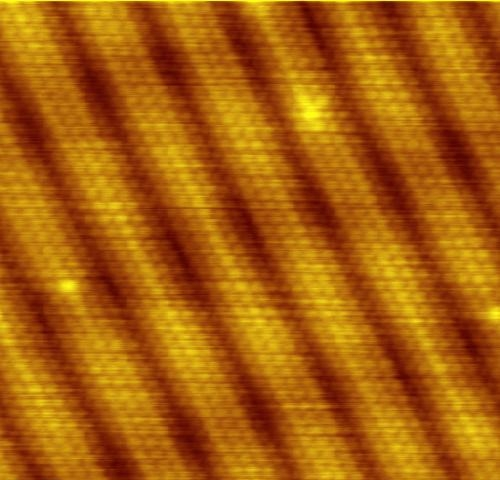
\includegraphics[width=0.6\linewidth]{Atomic_resolution_Au100.JPG}
	\caption{STM-bilde av 100-planet til gull som viser rekonstruksjon på overflaten. Atomene ordner seg i kolonner med tykkelse på noen få atomer, med gap mellom hver kolonne.}
	\label{fig:recAu}
\emd\end{figure}

I Figur \ref{fig:recAu} har man kuttet langs (100)-planet. Hvis man i stedet kutter langs (111)-planet, som har en heksagonal struktur, vil det i stedet dannes en fiskebein-struktur. Ved likevekt er det 23 overflateatomer på en avstand som tilsvarer 22 atomer i bulk, og dette kompenserer materialet for ved å lage ``folder'' slik at noen atomer er hevet med \SI{0.03}{\nano\meter} i forhold til noen andre atomer.

Både relaksasjon og rekonstruksjon fører at det oppstår mekanisk spenning, siden overflateatomene blir strukket eller sammentrukket i forhold til atomplanene under overflaten. Dette er analogt med overflatespenning for væsker. %

\paragraph{Vicinale overflater} Her er en fin måte å lage overflater med relativt lang periodisitet på: kutt en krystall langs et plan som er tettpakket, men bom med en vinkel $\theta$ mellom \SI{0}{\degree} og \SI{15}{\degree}. Siden det er vanskelig å kutte gjennom atomer, vil du få den beste mulige tilnærmingen: en atomær trapp der trinnene har høyde på ett atom og lengde på $L = \frac{d}{\tan\theta}$, som vist i Figur \ref{fig:vicinal}. 
\begin{figure}[H]
	\bmd\centering
	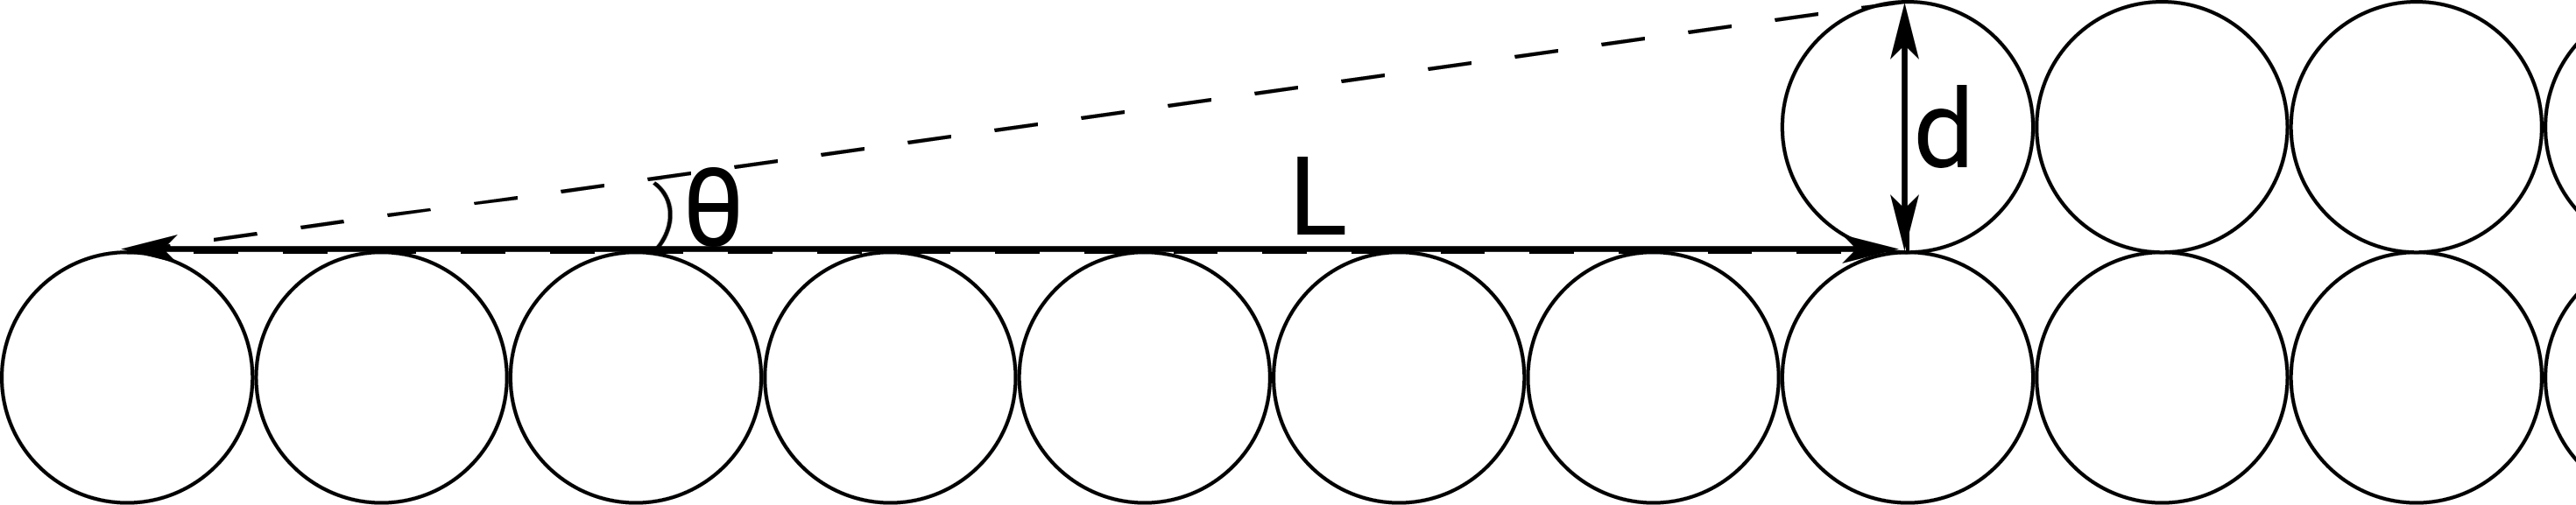
\includegraphics[width=\linewidth]{vicinal.png}
	\caption{Vicinal overflate}
	\label{fig:vicinal}
\emd\end{figure}
Gjennom en prosess som kalles fasettering vil overflaten så organisere seg på en måte som minimerer den frie energien i systemet.

Ved å stille inn $\theta$ slik du vil får du altså en periodisk struktur med rekker av atomer som er litt mer reaktive enn sine naboer (siden de er på en kant og ikke bare på en overflate), adskilt fra hverandre med et mellomrom på $L$.

% Det med oksygen og kobber
\paragraph{Kunstig mønstring} I tillegg til naturlige metoder for å lage mønstrede overflater kan vi også bruke litografi eller etsing til å lage mønstrede overflater.

\cstitletwo{Organisert vekst på et strukturert substrat}
Når man så lar materialet sitt adsorberes på substratet (ved en av metodene i neste delkapittel) kan vekst skje på tre måter, avhengig av balansen i fri energi mellom det adsorberte materialet (heretter adsorbatet), substratet og grenseflaten mellom de to. Dersom
\begin{equation}
	\gamma_{\text{substrat}} > \gamma_{\text{adsorbat}} + \gamma_{\text{grenseflate}}
\end{equation}
vil det første atomlaget av adsorbatet dekke hele substratet. La oss så kalle den nye frie energien for $\gamma_{\text{substrat}}'$, som nå tar hensyn til det nye laget av adsorbat og eventuelle stablefeil og dislokasjoner. Dersom vi nå har at 
\begin{equation}
	\gamma_{\text{substrat}}' > \gamma_{\text{adsorbat}} + \gamma_{\text{grenseflate}}
\end{equation}
vil påfølgende atomlag fortsette å dekke hele substratet, og adsorbatet dannes lag for lag. Denne typen vekst kalles FM-vekst (etter Frank-van der Merve), og er ikke så veldig interessant. 

Hvis $\gamma_{\text{substrat}}'$ derimot har blitt tilstrekkelig redusert, vil adsorbatet i stedet organisere seg i form av tredimensjonale klynger/øyer på toppen av det første laget. Denne typen vekst kalles \emph{Stranski-Krastanov}-vekst (SK-vekst på kort).

Dersom vi i utgangspunktet har 
\begin{equation}
	\gamma_{\text{substrat}} < \gamma_{\text{adsorbat}} + \gamma_{\text{grenseflate}}
\end{equation}
vil slike tredimensjonale klynger dannes direkte på substratet. Denne typen vekst kalles \emph{Volmer-Weber}-vekst (VW-vekst på kort). VW-vekst ser vi gjerne hvis et reaktivt materiale deponeres på et ikke-reaktivt substrat, for eksempel et overgangsmetall på et edelt metall.

I både SK- og VW-vekst dannes øyene gjennom nukleering og vekst. Atomene som når overflaten beveger seg rundt gjennom diffusjon, og det vil foregå nukleering der mange atomer møtes. Seinere i prosessen vil atomene begynne å sette seg på allerede eksisterende øyer i stedet for å begynne å lage nye øyer.

\cstitletwo{Vekst av indiumarsenid-kvanteprikker på galliumarsenid}

\paragraph{Balanse mellom overflateenergi/kurvatureffekter og elastisk energi} Det er en balanse mellom overflateenergi og elastisk energi som bestemmer hvordan øyene vokser. Man har et ledd i det kjemiske potensialet som avhenger av overflateenergi og forskyver likevekten mot vekst i konkave områder som groper og hull, men man har også et ledd assosiert med elastisk energi i bulk-atomene som forskyver likevekten mot vekst i konvekse områder som kanter og hjørner. % Skjønte ikke :(

Vi har eksempler på synteser der den ene eller den andre effekten dominerer. For eksempel: hvis vi vokser \ce{InAs} på \ce{GaAs} som man har laget sagtannform i ved å bruke interferometri og etse, vil vekst foregå på bunnen av de konkave områdene. Dette er fordi kurvatureffektene blir dominerende. Hvis vi derimot vokser \ce{InAs} på en flerlagsstruktur med \ce{In_{$x$}Ga_{$1-x$}As} mellom to lag av \ce{GaAs}, vil de elastiske effektene dominere slik at \ce{InAs} vokser på toppen av strukturen.

% MOAR!

%!TEX root = Nanomat.tex
\ctitletwo{NS6 Nye metoder for nanolitografi}
\addcontentsline{toc}{section}{NS6 NYE METODER FOR NANOLITOGRAFI}
Nanolitografi spiller en viktig rolle i fundamental forskning og i mange områder i forskningen. Litografi med fotoner, elektroner og ioner er fint, men vi støter på problemer med diffraksjon og spredning av partikler. Derfor har man utviklet alternative metoder som er fundamentalt forskjellige fra å skyte på substratet med partikler.

\cstitletwo{Nanoimprint-litografi (NIL)}
I nanoimprint-litografi har man et substrat, og resist spredt jevnt utover substratet, og så bruker man en støpeform til å presse en struktur inn i resisten (støpeformen kan man lage med andre mer tidkrevende metoder som elektronstråle-litografi, for når man først har laget formen kan man bruke den igjen og igjen). Etterpå bruker man RIE for å etse ned resisten, helt til man har etset bort de områdene av resisten som ble trykket ned. Deretter deponerer man metall og gjør lift-off. Med denne metoden kan man få resultater som er sammenlignbare med resultatene man får med andre litografiske metoder. Hvis man bruker varme mens man presser ned støpeformen, kalles prosessen \emph{termoplastisk nanoimprint-litografi}.

Fordeler med NIL er at man kan oppnå veldig høy oppløsning, det er billig og enkelt, det er lett å implementere, og det kan brukes i mange forskjellige situasjoner. Ulempen er at man trenger en støpeform som må varmes opp og kjøles ned.

\paragraph{Resisten} Vi bruker gjerne PMMA eller polykarbonat som resist. Imprinting gjøres ved en temperatur som er høyere enn glassomvandlingstemperaturen til resisten (altså der den begynner å bli myk og formbar), samtidig som man presser ned formen. Så senker man temperaturen samtidig som man trykker, for å gjøre resisten fast igjen. Så fjerner man støpeformen og sitter igjen med en negativ av støpeformen i resisten.

\paragraph{Tykkelsen til resisten er viktig} Tykkelsen man bør bruke på resisten avhenger av strukturen man ønsker å lage, eller mer spesifikt hvor stor andel av arealet til strukturen som skal trykkes ned. For å få korrekt resultat må forholdet mellom den opprinnelige tykkelsen $h_i$, tykkelsen $h_c$ til de nedtrykte områdene og tykkelsen $h_m$ til områdene som ikke trykkes ned, være
\begin{equation}
	h_i = h_c + fh_m,
\end{equation}
der $f$ er andelen av strukturen som er trykket ned og senere skal etses bort.

\paragraph{Triks for å øke maksimalt høyde/bredde-forhold} For å øke høyde/bredde-forholdet (aspect ratio) til strukturene (altså lage dype, men tynne kanaler i resisten) kan man bruke et lag av \ce{Ge}, som ikke blir etset ned av RIE i samme grad som PMMA. Det man gjør er å først legge på et lag av PMGI (en annen type resist som \emph{ikke} blir myk ved temperaturen som PMMA blir myk ved), så et lag av \ce{Ge}, og til slutt et lag av PMMA. Man presser inn strukturen i PMMA som vanlig, og etser bort så man har bar \ce{Ge} på områdene som ble trykt ned, og rester av PMMA på områdene man ikke trykte ned. Så bytter man til et annet løsemiddel som kun løser opp \ce{Ge}, men ikke PMMA. Dermed vil områdene som ble trykt ned være frie for \ce{Ge}, mens det fortsatt er \ce{Ge} på områdene som ikke ble trykt ned. Så bytter man tilbake til RIE, som etser bort PMGI men ikke \ce{Ge}. 

\paragraph{UV-nanoimprint-litografi} Dette er en variant av NIL der man bruker UV-lys i stedet for økt temperatur. Dette er naturligvis kjekt å ha hvis strukturene man skal lage ikke tåler høy temperatur. 

Beskrivelse av metoden kommer. 

\cstitletwo{Ander metoder}
\paragraph{Nanopreging / nanoembossing}
I denne metoden har man også en støpeform, men i dette tilfellet bruker man små kuler av materialet man vil lage en struktur i. Så presser man formen mot en flat \ce{Si}-wafer ved høy temperatur slik at materialet danner en negativ av støpeformen. Til slutt fjerner man det fra støpeformen og beundrer verket sitt.

\paragraph{Soft lithography}
Dette er som NIL, men støpeformen man bruker er laget av PDMS, som er bøyelig og fleksibelt. Dette gjør at man også kan mønstre bøyde overflater med en slik fleksibel støpeform. Ulempen ved denne metoden er at formen lettere blir deformert og fordreid.

\paragraph{Near-field lithography} Probemikroskoper som STM, AFM og SNOM kan også brukes til å manipulere overflater. Med STM kan man for eksempel flytte på enkeltatomer til formen man vil. Dette er naturligvis altfor sakte og lokalt til å være en fornuftig fabrikasjonsmetode.

\paragraph{Dip-pen lithography (DPN)} Med denne metoden har man en AFM-tipp som er dekket med en løsning av organiske molekyler (for eksempel tioler). Denne tippen fører man over et substrat (hvis vi bruker tioler vil substratet typisk være gull), og der man har pennen vil det deponeres tioler lokalt. Med denne metoden kan man lage kompliserte mønstre med forskjellige molekyler. Man kan også parallellisere prosessen ved å bruke mange tipper samtidig, og dermed få det til å gå temmelig raskt. I IBM sitt ``millipede''-system har man en oppstilling av 55000 AFM-tipper som kjører parallelt. 


\setcounter{section}{20}
\ctitle{Elektrostatisk potensial}
\paragraph{Dette kapittelet}
En mer ``standard'' behandling av elektrostatikk gir de samme resultatene. Vi går veldig fort gjennom dette, fordi det ikke er noe her som ikke er kjent fra et grunnkurs i elektromagnetisme.

\cstitle{Hva er elektrostatisk potensial?}
Arbeidet $\delta W$ som kreves for å bevege en ladning $q$ en liten distanse $d\vec{l}$ i et konstant elektrisk felt $\vec{E}$ er 
\begin{equation}
	\delta w = -\vec{f}\cdot d\vec{l}=-q\vec{E}\cdot d\vec{l}
\end{equation}
der minustegnet indikerer at arbeidet gjøres \emph{mot} feltet, og ikke av feltet.
For å bevege ladningen fra A til B kreves derfor
\begin{equation}
	w_{AB}=-q\int_{A}^B \vec{E}\cdot d\vec{l}
\end{equation}
Vi \emph{definerer} nå potensialforskjellen $\Delta \psi = \psi_{AB}$ som arbeidet som kreves for å bevege en testladning med størrelse 1 fra A til B:
\begin{equation}
	\Delta \psi = \psi_{AB}=\psi_B-\psi_A=\frac{W_{AB}}{q_{test}}=-\int_A^B\vec{E}\cdot d\vec{l}
\end{equation}
så det elektrostatiske potensialet ganger en ladning blir en energi.
Integralligningen er ekvivalent med differensialligningen i \eqref{enabla}.

\cstitle{Elektrostatiske interaksjoner er konservative}
Elektrostatisk arbeid er reversibelt og derfor veiuavhengig. Arbeidet som utføres for å flytte en ladning fra et punkt $A$ til et punkt $B$ via en bane $\mathscr{C}$. Videre summerer det elektrostatiske arbeidet opp til 0 dersom banen går tilbake til utgangspunktet.

\cstitle{Poissons ligning}
Er:
\begin{equation}
	\nabla^2\psi=-\frac{\rho}{\epsilon_0D}
\end{equation}
Merk at
\begin{equation}
	\nabla\cdot\vec{E}=-\nabla^2\psi.
\end{equation}
Det setter vi pris på.


\ctitle{Elektrokjemisk likevekt}
\paragraph{Dette kapittelet}
Elektrostatisk potensial og kjemisk potensial kan kombineres til én størrelse: elektrokjemisk potensial. Nernsts ligning kan utledes fra likevektsbetingelser. 


\cstitle{Elektrokjemisk potensial}
Den indre energien $U$ er en funksjon av ekstensive variable: $U=U(S,V,\vec{N})$. Nå utvider vi denne med ladningene i systemet, slik at $U=U(S,V,\vec{N},\vec{q})$. Med $M$ ladninger har vi nå at
\begin{equation}
	dU=TdS-pdV+\sum_{j=1}^{N}\mu_jdN_j+\sum_{i=1}^{M}\psi_idq_i
\end{equation}
der $\psi_i$ er det elektrostatiske potensialet som føles av ionet $i$. Ofte er $\psi_i=\psi$ det samme for alle $i$, siden $\psi$ gjerne kommer fra elektroder eller ladde flater.
Gibbs fri energi ($G=U+pV-TS$) blir
\begin{equation}
	\label{gibbsplusel}
	dG=-SdT+Vdp0\sum_{j=1}^N\mu_jdN_j+\sum_{i=1}^M\psi_idq_i
\end{equation}
I virkeligheten har vi løsninger med molekylære ioner. Hvert ion har ladning $z_ie$ (eksempel: i Cu$^{2+}$ er $z=2$), slik at bidraget fra hvert specie er $q_i=z_ieN_i$. Siden det kjemiske potensialet kommer fra de samme speciene, blir \eqref{gibbsplusel} til
\begin{equation}
	dG=-SdT+Vdp+\sum_{j=1}^N(\mu_j+z_ie\psi_i)dN_i
\end{equation}
Nå definerer vi \i{elektrokjemisk potensial} som
\begin{equation}
	\mu_i'=\mu_i+z_ie\psi_i
\end{equation}
Ved konstant $p$ og $T$ inntreffer likevekt når det elektrokjemiske potensialet er likt overalt.

\paragraph{Tolkning av det elektrokjemiske potensialet}
Mens det kjemiske potensialet er den frie energien som kreves for å sette inn en partikkel, er det elektrokjemiske potensialet den frie energien som kreves for å sette inn et elektronøytralt ione\emph{par}. Dette er fordi vi har en veldig sterk, implisitt begrensning: elektronøytalitet må bevares.

\cstitle{Nernsts ligning}
Elektrostatisk potensial er en funksjon av posisjonen: $\psi = \psi(\vec{r})$. Vi behandler det enkle endimensjonale tilfellet $\psi=\psi(x)$ i en løsning som kun inneholder étt ionisk specie. Et ion kan befinne seg i posisjon $x_1$ eller i posisjon $x_2$. Da er likevektsbetingelsen at
\begin{equation}
	\label{elpoteq}
	\mu'(x_1)=\mu'(x_2)
\end{equation}
Vi har fra før av at det kjemiske potensialet er $\mu(x)=\mu^o+k_BT\ln c(x)$ (der $c(x)$ er konsentrasjonen), slik at
\begin{equation}
	\label{elpotget}
	\mu'(x)=\mu^o+k_BT\ln c(x)+ze\psi(x)
\end{equation}
Så setter vi inn \eqref{elpotget} i \eqref{elpoteq} og får ut \i{Nernsts ligning}:
\begin{equation}
	\label{nernst}
	\ln\frac{c(x_2)}{c(x_1)}=-\frac{ze(\psi(x_2)-\psi(x_1))}{k_BT}
\end{equation}
En annen form for ligningen som kan være nyttig for å regne ut konsentrasjonen på ett sted basert på konsentrasjonen på et annet sted, er
\begin{equation}
	c(x_2)=c(x_1)e^{-\frac{1}{k_BT}ze(\psi(x_2)-\psi_(x_1))}
\end{equation}

Merk at dette er en generell fremgangsmåte for å utvide termodynamikken med en energi avhenger av posisjonen i rommet.

\paragraph{Nøytrale salter} For et salt som ioniserer, for eksempel NaCl, er 
\begin{equation}
	\mu_{NaCl}=\mu'_{Na^+}+\mu'_{Cl^-}
\end{equation}
eller
\begin{align}
\begin{split}
	\mu_{NaCl}=\mu_{Na^+}^o&+k_BT\ln c_{Na^+}+e\psi_{Na^+}\\+\mu_{Cl^-}^o&+k_BT\ln c_{Cl^-}-e\psi_{Cl^-}
\end{split}
\end{align}
Når $\psi$ er uavhengig av romlig posisjon, må $\psi_{Na^+}=\psi_{Cl^-}$ på grunn av ladningsbevaring. Derfor er
\begin{equation}
	\mu_{NaCl}=\mu_{NaCl}^o+2k_BT\ln c_{NaCl}
\end{equation}
Denne forenklingen fungerer ikke hvis saltet ikke er fullstendig løselig, slik at $\mu_{NaCl}\neq\mu_{Na^+}$, eller hvis det befinner seg nær store ladde overflater som kolloider, slik at $\psi$ avhenger av rommet.

Se slide 8/14 og 9/14 for en utledning av at
\begin{equation}
	\mu_l=\mu_l^o+k_BT\ln\frac{[C]^c}{[A]^a[B]^b}=\mu_l^o+k_B\ln Q
\end{equation}

\paragraph{Nernsts ligning for en elektrode} Vi ser på reaksjonen $M^{z+}+ze^-\rightarrow M$. Ved likevekt er $\mu_{s}'=\mu_{l}'$ (det elektrokjemiske potensialet for det faste stoffet er det samme som for den delen av stoffet som er løst opp i væske).
I væskefasen er 
\begin{equation}
	\mu'_l=\mu_l^o+k_BT\ln Q+ze\psi_l
\end{equation}
I fast stoff sier vi at $Q=1$ (per konvensjon), slik at
\begin{equation}
	\mu'_s=\mu_s^o+ze\psi_s
\end{equation}
Ved likevekt har vi da at
\begin{equation}
	\mu_l^o+k_BT\ln Q+ze\psi_l=\mu_s^o+ze\psi_s
\end{equation}
Vi grupperer sammen de materialavhengige størrelsene som vi ikke er i stand til å måle på en side:
\begin{equation}
	ze\psi_0=\mu_s^o+ze\psi_s-\mu_l^o
\end{equation}
der $\psi_0$ kalles \i{halvcellepotensialet} for den gitte reaksjonen ved elektroden. Halvcellepotensialet slås opp i tabell. Vi har nå at
\begin{equation}
	ze\psi_l=ze\psi_0-k_BT\ln Q
\end{equation}
\i{Faradays konstant} er definert som $F=eN_A$. Hvis vi i tillegg husker at $R=N_Ak_B$, får vi uttrykket som man er vant til fra kjemien:
\begin{equation}
	\psi_l=\psi_0-\frac{RT}{zF}\ln Q
\end{equation}
Merk: ofte forenkler vi til $\psi\approx\psi_l$.

\paragraph{Nernsts ligning i en elektrokjemisk celle} Vi ser på reaksjonen $A(s)+B^{z+}\rightarrow A^{z+}+B(s)$. Potensialforskjellen mellom dem er
\begin{equation}
	\Delta \psi=\psi_{0,B}-\psi_{0,A}-\frac{RT}{zF}\ln Q
\end{equation}
Halvcellepotensialene måles i forhold til hverande (vi er aldri interessert i absoluttverdien), og man bruker en hydrogenelektrode som referanse ($\psi_{0,H_2}=0V$). 


%!TEX root = Nanomat.tex
\ctitle{Selvorganisering av magnetiske nanopartikler}
I dette kapittelet fortsetter vi på forrige kapittel, men fokuserer på systemer der de magnetiske egenskapene til partiklene bestemmer egenskapene til produktet. Som i forrige kapittel begynner vi med en væske med nanopartikler -- når disse er magnetiske kaller vi væsken et \emph{ferrofluid}. Strukturene vi observerer etter å ha deponert et ferrofluid og latt løsemiddelet fordampe, har ofte sammenheng med strukturene som allerede eksisterer i ferrofluidet. 

\paragraph{Motivasjon} Polykrystalline magnetiske materialer består gjerne av flere magnetiske domener (men magnetiske domener trenger ikke å ha noe å gjøre med korngrensene). En enkelt nanopartikkel er så liten at hele partikkelen kan være ett bestemt magnetisk domene. Dersom man kan ordne magnetiske nanopartikler på riktig måte, kan man få en lagringstetthet som er mye større enn i dagens harddisker, som er basert på \ce{CoCr}-legeringer.

\paragraph{Ting som kan påvirke de magnetiske egenskapene til nanopartikler} I tillegg til de iboende magnetiske egenskapene til materialet man jobber med (f.eks at jern er ferromagnetisk, mens sølv ikke er det), kan de magnetiske egenskapene til nanopartikler påvirkes av ting som avstand mellom partikler, temperatur under annealing, og surfaktanter eller andre molekyler som adsorberes på overflaten av partiklene.

\paragraph{Krav for at en sammensetning av magnetiske nanopartikler skal fungere} Det er noen ekstra krav forbundet med magnetiske nanopartikler:
\begin{itemize}
	\item Nanopartiklene må danne en veldig regulær 2D-struktur som dekker en størrelse på ca. \SI{200}{\nano\meter}. Vi må altså fortsatt ha en veldig spiss størrelsesfordeling.
	\item Orienteringen til de magnetiske dipolene må være stabil ved temperaturen der man skal bruke produktet. Dette er et problem hvis vi skal bruke nanopartikler, siden energien som kreves for å snu magnetiseringen på en partikkel er proporsjonal med volumet til partikkelen: $\Delta E = KV$. Her er $K$ \emph{anisotropi-konstanten} til materialet, så vi ønsker å bruke materialer der denne konstanten er høy. 
	\item Det må være mulig å lese og skrive informasjon til produktet. Hvert område som skal representere en bit, må kunne måles og manipuleres på en fornuftig måte.
\end{itemize}

\paragraph{Selvorganisering av magnetiske nanopartikler uten et eksternt felt: hvilken effekt har partiklenes størrelse og form?} Når vi ikke bruker et eksternt magnetfelt, er det nanopartiklenes magnetiske egenskaper samt størrelse og form som bestemmer hva slags struktur vi ender opp med. En fellesnevner for magnetiske nanopartikler er at de gjerne danner kjeder som minimerer energien forbundet med magnetismen. Kjeder oppstår når de attraktive kreftene forbundet med de magnetiske dipolene er mye større enn den termiske energien i miljøet (den termiske energien ``ønsker'' jo å spre partiklene i en tilfeldig konfigurasjon for å maksimere entropien). Jo større partiklene blir, jo større blir magnetismen i forhold til den termiske energien, og jo mer vil partiklene foretrekke å danne kjeder.

Sfæriske partikler får sin mest stabile posisjon når sørpolen hos én partikkel er i kontakt med nordpolen på den andre. Hvis partiklene er avlange, og magnetiseringsvektoren er i lengderetningen, vil den mest stabile konfigurasjonen være den der de står side ved side, med alternerende retning på magnetiseringen.

\paragraph{Selvorganisering av magnetiske nanopartikler med et eksternt felt som står normalt på substratet} La oss først se på tilfellet der vi bruker et eksternt felt som står normalt på substratet, samtidig som vi lar løsemiddelet i ferrofluidet fordampe. La oss også anta at vi bruker nanopartikler av kobolt, fordi det er det noen gjorde en gang. 

Hvis det eksterne feltet er svakt, vil nanopartiklene samle seg i dotter, som organiserer seg i en heksagonal struktur.

Hvis det eksterne feltet er sterkt, vil det dannes et labyrintaktig system av kanaler. Denne strukturen minner om strukturen man får når man lar en legering stivne ved det eutetiske punktet, og oppstår på grunn av det samme overordnede prinsippet: i begge tilfeller dannes kanalene på grunn av konkurranse mellom attraktive krefter med kort rekkevidde, og frastøtende krefter med lang rekkevidde. I tilfellet med de magnetiske nanopartiklene er de attraktive kreftene de samme som i forrige kapittel (overflatespenning mellom ferrofluidet og omgivelsene fører til at partiklene trekkes mot hverandre). De frastøtende kreftene oppstår på grunn av interaksjoner mellom det eksterne feltet og nanopartiklene.

La oss se på det kvantitativt. Den attraktive energien er
\begin{equation}
	E_a = \sigma A,
\end{equation}
der $\sigma$ er overflatespenning og $A$ er arealet til fluidet. Den frastøtende energien er
\begin{equation}
	\label{eq:mag_force}
 	E_m=\frac{-\mu_0}{2}\left<M\right>H_0LA',\footnote{...señorita.}
 \end{equation} 
der $H_0$ er det eksterne magnetiske feltet og $\left<M\right>$ er den gjennomsnittlige magnetiseringen til strukturen. $LA'$ er volumet til ferrofluidet, men $A'$ inneholder kun den delen av ferrofluidet som dekker substratet. $L$ er høyden på strukturene som oppstår.

$M$ er den totale magnetiseringen og oppstår både på grunn av det eksterne feltet $H_0$, og på grunn av feltet som oppstår når de magnetiske partiklene orienterer seg i motsatt retning av det eksterne feltet (la oss kalle det $H_d$). Altså er den totale magnetiseringen alltid mindre enn magnetiseringen på grunn av $H_0$. Uttryket for $M$ er 
\begin{equation}
	M = \chi(H_0+H_d),
\end{equation}
der $\chi$ er den magnetiske susceptibiliteten fra Elektromagnetisme. $H_0$ og $H_d$ har naturligvis motsatt fortegn, og $H_0$ har større absoluttverdi enn $H_d$. Når strukturer dannes, blir absoluttverdien til $H_d$ mindre, så da blir absoluttverdien til $M$ større. Denne effekten blir større jo større bredden på kanalene er. Dermed blir også absoluttverdien til $E_m$ større jo større kanalene er, jfr. ligning \eqref{eq:mag_force}.

Likevekt oppstår der $E_i + E_m$ er på sitt laveste, altså ved minimum for
\begin{equation}
	E_{\text{tot}} = \sigma A - \frac{-\mu_0}{2}\left<M\right>H_0LA'.\footnote{(hun svarte meg aldri, 'cause she ain't no $H_0LA'$-back girl)}
\end{equation}
Det som systemet ``selv'' kan endre er $A$, $A'$ og $L$. Systemet vil endre disse til det når minimum, og dette avhenger igjen av $H_0$. Når $H_0$ er liten vil $E_{\text{tot}}$ ha sitt minimum når labyrintene er ganske brede (i grensetilfellet med et veldig svakt felt vil labyrintene være så brede at de ikke lenger er labyrinter, men heller den ovennevnte strukturen med dotter i et heksagonalt gitter). Når $H_0$ er stor vil $E_{\text{tot}}$ ha sitt minimum når labyrintene er relativt smale.

\paragraph{Selvorganisering av magnetiske nanopartikler med et eksternt felt som går parallelt med substratet} I dette tilfellet har vi ikke like gode teoretiske modeller for å beskrive strukturene som oppstår. Det som er å si om dette tilfellet er at det er litt som tilfellet uten noe felt -- det vil dannes kjeder på grunn av interaksjoner mellom partikler. Siden vi har et eksternt felt, vil disse kjedene gå parallelt med det eksterne feltet. Det vil også være attraktive interaksjoner mellom kjeder, som fører til at det dannes sigarformede sammensetninger parallelt med det eksterne feltet.


%!TEX root = Nanomat.tex
\ctitle{Å lage tynnfilmer med våtkjemiske metoder}
I dette og neste kapittel skal vi lage tynnfilmer på et substrat. I dette kapittelet ser vi på våtkjemiske metoder (``wet-chemical methods''). Dette betyr i praksis at vi begynner med en løsning eller suspensjon med kildematerialet, og prøver å bruke denne til å dekke substratet.

\cstitle{Surfaktant-tynnfilmer}
\paragraph{Self-assembled monolayers (SAMs)} SAMs er akkurat det de høres ut som - todimensjonale enkeltlag med molekyler på substratet, som organiserer seg selv. SAMS lages ved at man drypper en passende løsning med surfaktanter på et substrat (eller dekker substratet i løsning). Så lener man seg tilbake og venter på at molekylene organiserer seg selv. 

Molekylene det er snakk om i SAMs er surfaktanter. Surfaktantene består av et hydrofilt hode, en alkyl-kjede og en funksjonell gruppe. Disse må oppfylle følgende krav:
\begin{itemize}
	\item Surfaktantens hode må være slik at det foretrekker å kjemisorberes på overflaten av substratet. 
	\item Svake bindinger mellom alkylkjedene sørger for selvorganiseringen.
	\item Hvilken funksjonell gruppe man har på enden av molekylet, avhenger av hvilke egenskaper man vil at filmen skal ha. 
\end{itemize}

Slik dannes SAMs:
\begin{enumerate}
	\item Surfaktanthodene kjemisorberes på substratet. Dette går kjapt, for kjemisorbsjonen er ganske eksoterm hvis vi har vært lure med valg av surfaktant og substrat. Surfaktantene vil prøve å komme seg inn på hvert eneste mulige bindingspunkt på substratet.
	\item Molekylene organiserer seg selv på overflaten gjennom diffusjon, van der Waals-krefter og elektrostatiske krefter. Det har seg slik at den frie energien er minimert når molekylene danner et ganske tettpakket 2D-lag på overflaten av substratet.
\end{enumerate}

Det finnes flere eksempler på materialer vi kan bruke til surfaktanter og til substrater, og bindingen mellom surfaktant og substrat kan være alt mulig:
\begin{itemize}
	\item Alkantioler (\ce{SH-(CH2)_{n}-R}) på en overflate av \ce{Au}, \ce{Ag} eller \ce{Cu}. I dette tilfellet vil det skje en oksidasjonsreaksjon der \ce{S-H}-bindingen brytes, og det dannes \ce{S-M}-bindinger samt hydrogengass. Dialkylsulfider og dialkyl-disulfider funker også -- svovel er generelt glad i disse metallene. I dette tilfellet vil det være en polar kovalent binding mellom svovel og metallet.
	\item Alkoholer og aminer på \ce{Pt}. I dette tilfellet vil det være ionebinding mellom surfaktanten og metallet.
	\item Karboksylsyrer på \ce{AlO} eller \ce{Ag}. Også her blir det ionebinding.
	\item Organosilisium-molekyler der surfaktanthodet er \ce{SiO2}, på et substrat av \ce{Si}. Eller surfaktanthodet kan være \ce{Al2O3} og substratet kan være \ce{Al} eller glass. I dette tilfellet vil det bli en kovalent binding mellom surfaktant og substrat. Hvis den funksjonelle gruppen på surfaktanten er \ce{OH}, kan vi faktisk lage en ny SAM på toppen av det første laget (og slik kan vi fortsette). Men merk at kvaliteten på de øvre lagene ikke vil være like god som kvaliteten på det første laget.
\end{itemize}

\paragraph{Languir-Blodgett-filmer}
Languir-Blodgett-filmer lages ved å dyppe substratet i en væske som har surfaktanter på overflaten, samtidig som man bruker en maskin til å dytte surfaktantene inn på substratet. Det forklares best med en figur:
\begin{figure}[H]
	\bmd\centering
	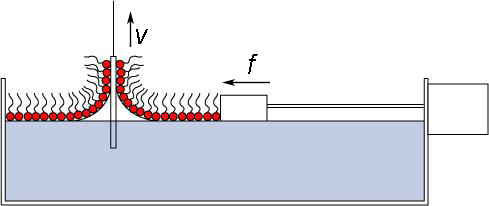
\includegraphics[width=\linewidth]{metodefigs/lb.png}
	\caption{Slik kan man lage Langmuir-Blodgett-filmer.  (av Dbroesch på Wikimedia, lisensiert under CC-BY-SA 3.0)}
	\label{fig:label}
\emd\end{figure}
De viktigste forskjellene mellom SAM og Langmuir-Blodgett-filmer er at I SAMs adsorberes surfaktantene via en kjemisk reaksjon (kjemisorpsjon), mens i Langmuir-Blodgett-filmer adsorberes surfaktantene ved hjelp av de mekaniske kreftene fra maskinen (fysisorpsjon). Dessuten lages ikke Langmuir-Blodgett-filmer ved self-assembly (vi bruker eksterne krefter til å lage filmen).

\cstitle{Chemical solution deposition}
I de tre neste metodene -- dipcoating, spincoating og spraycoating -- begynner vi med en kjemisk løsning, som vi så forsøker å dekke substratet med. Chemical solution deposition er vanlig å bruke med sol-gel-metoder. 

\paragraph{Dipcoating} er veldig enkelt. Dypp substratet i en løsning med det du vil lage tynnfilm av, og trekk den opp. Det viser seg at tykkelsen på filmen er proporsjonal med 
\begin{equation}
	\sqrt{\frac{\eta U_0}{\rho g}},
\end{equation}
 der $\eta$ er viskositeten til løsningen, $U_0$ er hastigheten substratet trekkes opp med, $\rho$ er tettheten til sol-en som dekker substratet, og $g$ er jordakselerasjonen. Merk at filmen blir \emph{tykkere} jo raskere man drar substratet opp, i motsetning til hva man kanskje skulle tro. Jeg har ikke funnet ut hvorfor, men jeg regner med at det er fordi filmen ikke rekker å renne av substratet.
\begin{figure}[H]
\bmd\centering
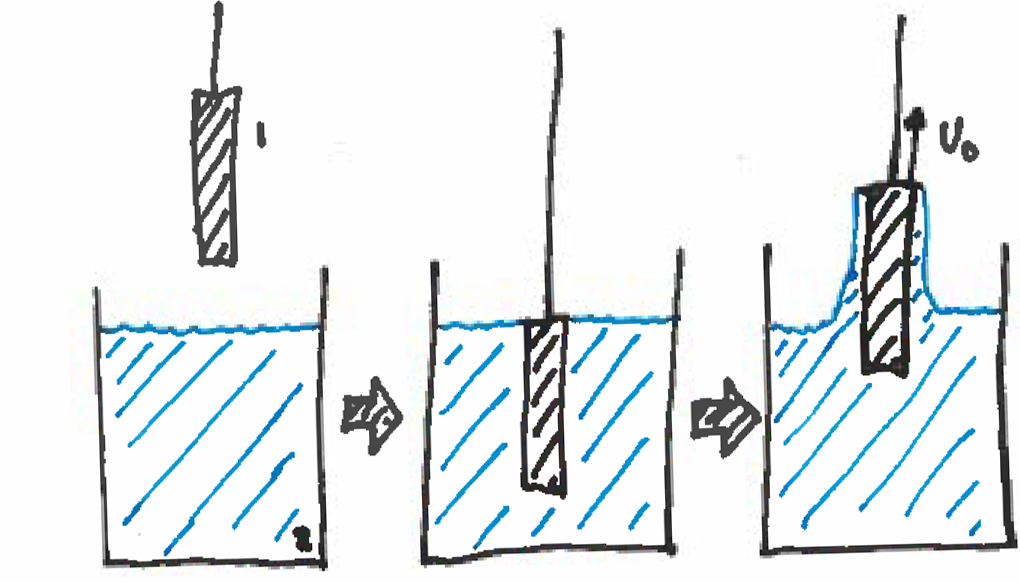
\includegraphics[width=\linewidth]{metodefigs/dipcoat.png}
\caption{Sånn kan man gjøre dip coating. 1: Substrat. 2: Løsning eller suspensjon.}
\emd\end{figure}
Dipcoating kan enkelt parallelliseres (bare dypp en rekke substrater i samme løsning) og kan dermed gjøres på stor skala. Hvis substratet er fleksibelt, kan man videre effektivisere ved å ha substratet på en rull, og kontinuerlig trekke det gjennom løsningen:
\begin{figure}[H]
	\bmd\centering
	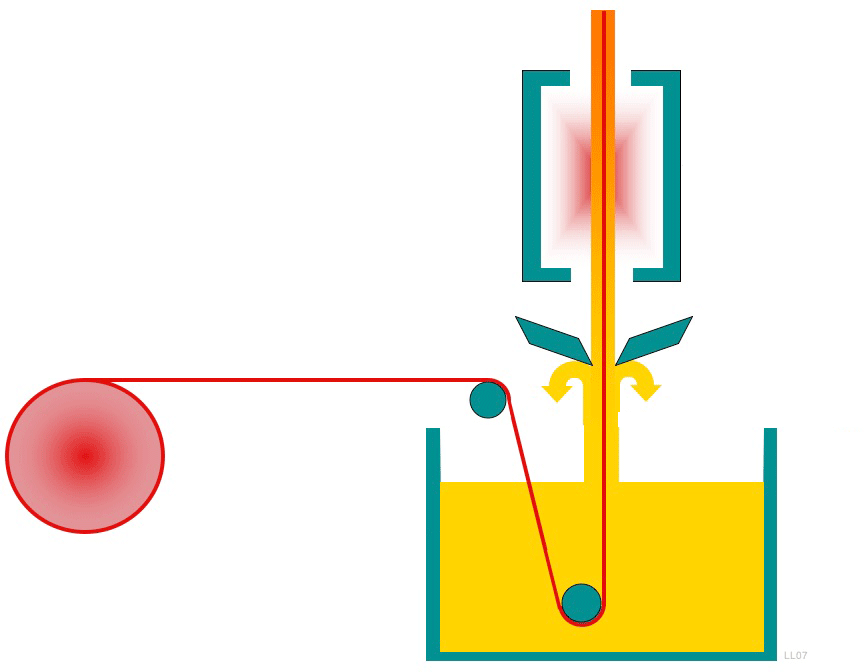
\includegraphics[width=0.8\linewidth]{metodefigs/dipcoatcont.png}
	\caption{Sånn kan man også gjøre dip coating.}
\emd\end{figure}

\paragraph{Spincoating} er også temmelig enkelt: du drypper en passende mengde av løsningen din på substratet. Dette substratet har du festet til en disk, som spinner med høy hastighet for å fordele løsningen jevnt utover substratet. Tykkelsen på filmen blir da proporsjonal med (blant annet)
\begin{equation}
	\frac{\eta}{\omega^2},
\end{equation}
der $\omega$ er vinkelfrekvensen til disken. Andre faktorer som påvirker tykkelsen og mikrostrukturen til filmen er måten løsningen dekker substratet på, tiden man bruker på å spinne, mengden løsning man putter på, pH, antall lag man putter på, og tørking/oppvarming etter at man har spunnet disken. Avhengig av disse parametrene kan man få defekter som luftbobler, ujevn filmtykkelse og spiralmønstre i filmen.
\begin{figure}[H]
\bmd\centering
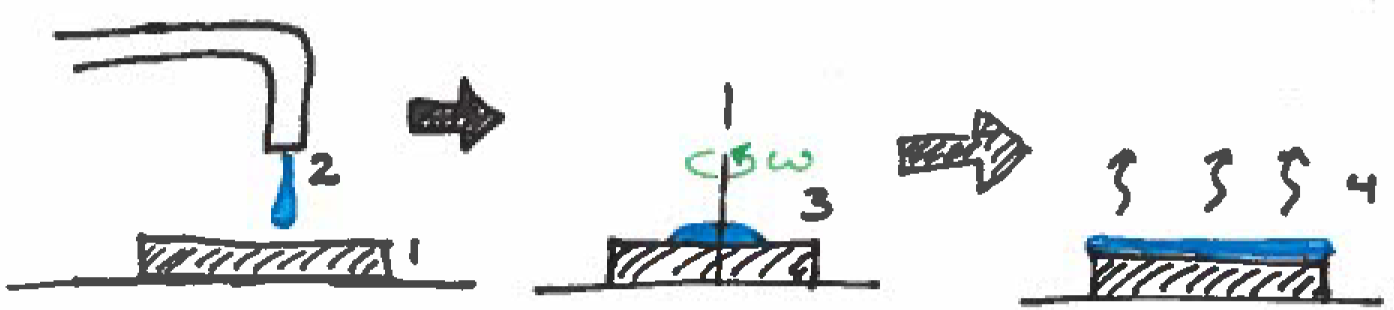
\includegraphics[width=\linewidth]{metodefigs/spincoat.png}
\caption{Sånn kan man gjøre spin coating. 1: Substrat. 2: Løsning dryppes på substratet. 3: Rotasjon sprer løsningen som en jevn film gjennom sentrifugalkrefter. 4: Løsemiddelet fordamper.}
\emd\end{figure}
Spincoating er ikke like enkelt å oppskalere som dipcoating, for du må jo feste og spinne hver enkelt disk hver for seg.

\paragraph{Problemer med dip- og spincoating} Hovedproblemet med de to ovennevnte metodene er at det fort kan dannes sprekker i filmen. Dette kan skje hvis
\begin{enumerate}
	\item gel-en begynner å krympe for mye når løsemiddelet fordamper
	\item det begynner å bli polymerisering og krysslinking i gel-matrisen
	\item kapillærkrefter trekker og strekker på gel-en (også på grunn av fordamping av løsemiddelet, se kapittelet om sol-gel)
	\item substratet og filmen har forskjellige varmeutvidelseskoeffisienter
\end{enumerate}
Vi kan unngå sprekkdannelse ved å
\begin{enumerate}
	\item la filmen ha større bruddseighet (duh)
	\item la filmen være mer elastisk (lavere Youngs modulus)
	\item redusere mengden løsemiddel i løsningen når den begynner å stivne
	\item redusere tykkelsen på filmen
\end{enumerate}

\paragraph{Spray coating} Du har en gass-strøm som trekker med seg kjemiske forløpere til filmen i en spray.
\begin{figure}[H]
\bmd\centering
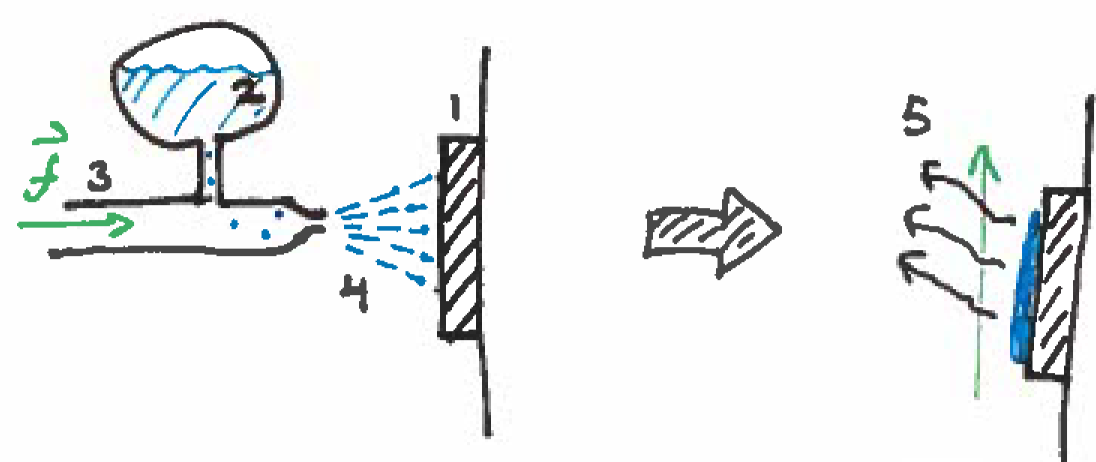
\includegraphics[width=0.7\linewidth]{metodefigs/spraycoat.png}
\caption{Sånn kan man gjøre spray coating. 1: Substrat. 2: Løsning. 3/4: Løsningen blåses mot substratet i form av en spray som treffer substratet. 5: Løsemiddel samt dråper og pulver av løsningen blåses vekk.}
\emd\end{figure}
Dette er veldig enkelt, kan gjøres ved lav temperatur, er lett å skalere opp og automatisere, og kan gjøres med en rekke forskjellige materialer på en rekke forskjellige substrater. Det kan brukes til å lage dopede eller graderte filmer, eller filmer som består av flere lag.

Dessverre er metoden sensitiv for støv, det er ikke lett å få en film med uniform tykkelse, og det er nødvendig med varmebehandling til slutt for å få filmen tett og sterk nok.

\paragraph{Bruksområder for dip- og spin coating} Filmene vi lager med de to ovennevnte metodene kan brukes til å lage beskyttende belegg (mot korrosjon og oksidasjon), optiske belegg (for å forbedre speil og linser), fotosensitive resister i litografi, og ferromagnetiske belegg i datamaskinminne. Vi kan også lage belegg som endrer egenskapene til overflater (for eksempel ved å gjøre dem glattere eller vannavstøtende), eller bruke dem til å lage systemer for drug-delivery.

\paragraph{Elektrokjemisk deponering} er å lage en reversert galvanisk celle der katoden er substratet. Kationer i løsningen går mot substratet og inngår i en reduksjonsreaksjon der. 
\begin{figure}[H]
\bmd\centering
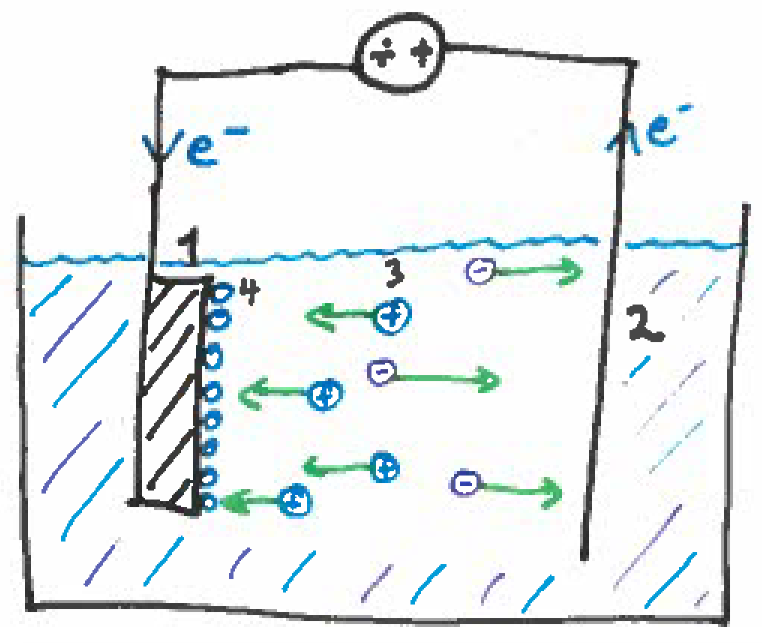
\includegraphics[width=0.6\linewidth]{metodefigs/elkjemdep.png}
\caption{Sånn kan man gjøre elektrokjemisk deponering. 1: Substrat (også katoden). 2: Anode. 3: Kationene i løsningen går mot katoden. 4: Kationene reduseres på substratet og danner en (elektrisk ledende) film.}
\emd\end{figure}
Metoden er fin for å lage tynnfilmer av metaller, for det er i hovedsak ledningsevnen til substratet (og den deponerte filmen) som bestemmer prosessforløpet. Siden substratet skal være en elektrode, må det være elektrisk ledende. Og hvis filmen ikke er ledende, vil deponeringen stoppe når det første laget har dannet seg på elektroden. Så: jo lavere konduktiviteten til filmen er, jo mindre blir den maksimale tykkelsen til filmen. Filmen blir også mer ujevn hvis materialet er en dårlig leder.

Hvis reduksjonspotensialet til materialet man skal deponere er lavere enn reduksjonspotensialet til vann, altså hvis det er et veldig edelt metall, kan man ikke bruke vann. Dette fordi du ender opp med å hydrolysere vannet i stedet (samme problem som i Cushing, da vi skulle bruke reduksjon av metall til å lage nanopartikler). I så fall må man bruke ikke-vandige løsemidler eller en saltsmelte.

\paragraph{Elektroforetisk deponering} er elektrokjemisk deponering der du bruker en suspensjon av kolloidale partikler i stedet for en løsning. Disse kolloidale partiklene må være elektrisk ladet i suspensjonen, men de trenger ikke å være elektrisk ledende. Ellers gjelder de samme prinsippene som for elektrokjemisk deponering.

I dette tilfellet slipper vi som regel problemene med egenelektrolyse av vann, for det er ikke en reduksjonsreaksjon som forårsaker filmdannelse -- det er det elektriske feltet mellom elektrodene som trekker partiklene mot den ene elektroden.

En ulempe med elektroforetisk deponering er at du ikke kan lage veldig tynne filmer med denne metoden - filmens tykkelse er begrenset av størrelsen til partiklene.


%!TEX root = Nanomat.tex
\ctitle{Å lage tynnfilmer med CVD og PVD}
I dette kapittelet fortsetter vi å lage tynnfilmer, men i dette tilfellet er forløperne til tynnfilmen i ``dampfase'' (vapor-phase). I \emph{Chemical Vapor Deposition (CVD)} har vi en damp av molekyler, og i \emph{Physical Vapor Deposition (PVD)} har vi en damp av atomer.

\paragraph{Generelle ting å tenke på}
Kontroller substrattemperatur og deponeringstemperatur, hold dem så lave som mulig (for å gjøre dette bruker vi gjerne plasma - plasma sørger for høy mobilitet og reaktivitet selv ved lave temperaturer). Dette for å hindre ukontrollert kornvekst og diffusjon mellom lag i flerlagsfilmer. 

\cstitle{Chemical Vapor Deposition (CVD)}
I CVD introduserer vi gasser i den ene enden av et kammer, lar disse gassene diffundere og reagere for å danne en tynnfilm på et substrat, og fjerner biprodukter fra den andre enden av kammeret. Den generelle flyten i CVD er beskrevet i figuren, men det finnes mange forskjellige varianter av CVD som på den ene eller den andre måten gjør prosessen mer effektiv.

\begin{figure}[H]
\bmd\centering
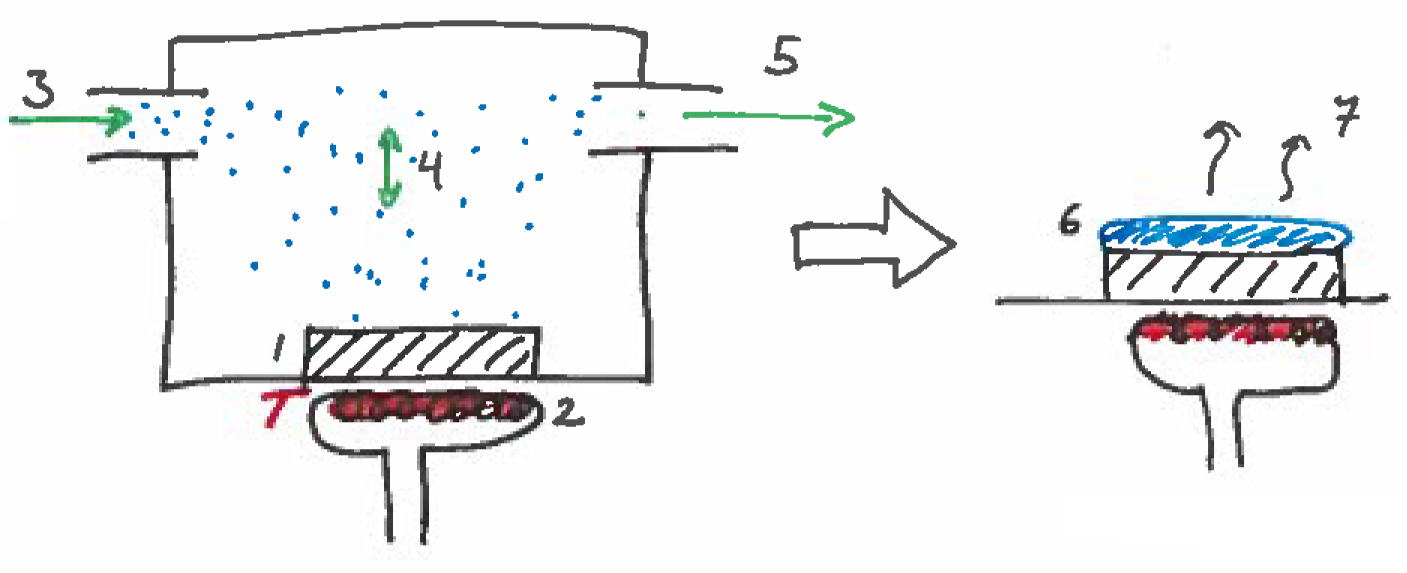
\includegraphics[width=\linewidth]{metodefigs/cvd.png}
\caption{Sånn kan man gjøre CVD. 1: Substrat. 2: Varme. 3: Gass med de kjemiske forløperne til filmen kommer inn i kammeret. 4: Gassen diffunderer på tvers av luftstrømmen. 5: Gassen pumpes ut av kammeret ved vakuum. 6: Overflatereaksjoner på substratet fører til at en film dannes. 7: Eventuelle biprodukter må vekk fra filmen.}
\emd\end{figure}

Gassene kan enten: reagere mens de er i ``lufta'', og så bli deponert på substratet; eller de kan vente med å reagere til de har landet på substratet. For å aktivere de kjemiske reaksjonene kan vi enten bruke varme, eller vi kan bruke plasma. Hvis vi bruker varme kalles det en \emph{termisk aktivert CVD-prosess}, og her kan vi velge mellom å bruke en ``hot-walled reactor'' (der hele reaktoren varmes opp) eller en ``cold-walled reactor'' (der kun substratet varmes opp). Temperaturen i termisk aktiverte CVD-prosesser er gjerne \SI{1200}{\kelvin} eller høyere. Hvis vi i stedet velger å bruke plasma til å aktivere reaksjonene, klarer vi oss med en lavere temperatur.

Noen av fordelene og ulempene med CVD:
\begin{itemize}
	\item Vi kan gro filmer med forholdsvis høy hastighet (noen mikrometer pr. time)
	\item Vi kan gro filmer som har uniform tykkelse, også hvis substratet har en meget funky form
	\item Gassene som brukes i CVD er ofte giftige eller farlige på andre måter
	\item Man kan lage alt mulig rart av tynnfilmer med CVD avhengig av hvilke gasser man introduserer i kammeret.
	\item Temperaturen i termisk aktiverte CVD-prosesser er upraktisk høy. Hvis vi bruker plasma (neste avsnitt) kan vi gjøre temperaturen mer levelig.
\end{itemize}
Før vi ser på plasma-aktivert CVD, må vi finne ut hvordan man lager plasma:

\paragraph{DIY guide: hvordan lage plasma} En vanlig måte å lage plasma på, er å putte en gass (for eksempel \ce{Ar}) i et kraftig elektrisk felt som alternerer med en frekvens på rundt \SI{13.56}{\mega\hertz} (som er i frekvensområdet til høyfrekvente radiobølger). Da vil elektronene på en måte ristes løs fra argonkjernen, fordi elektronet akselereres mye mer enn den tyngre argonkjernen.
\begin{figure}[H]
\bmd\centering
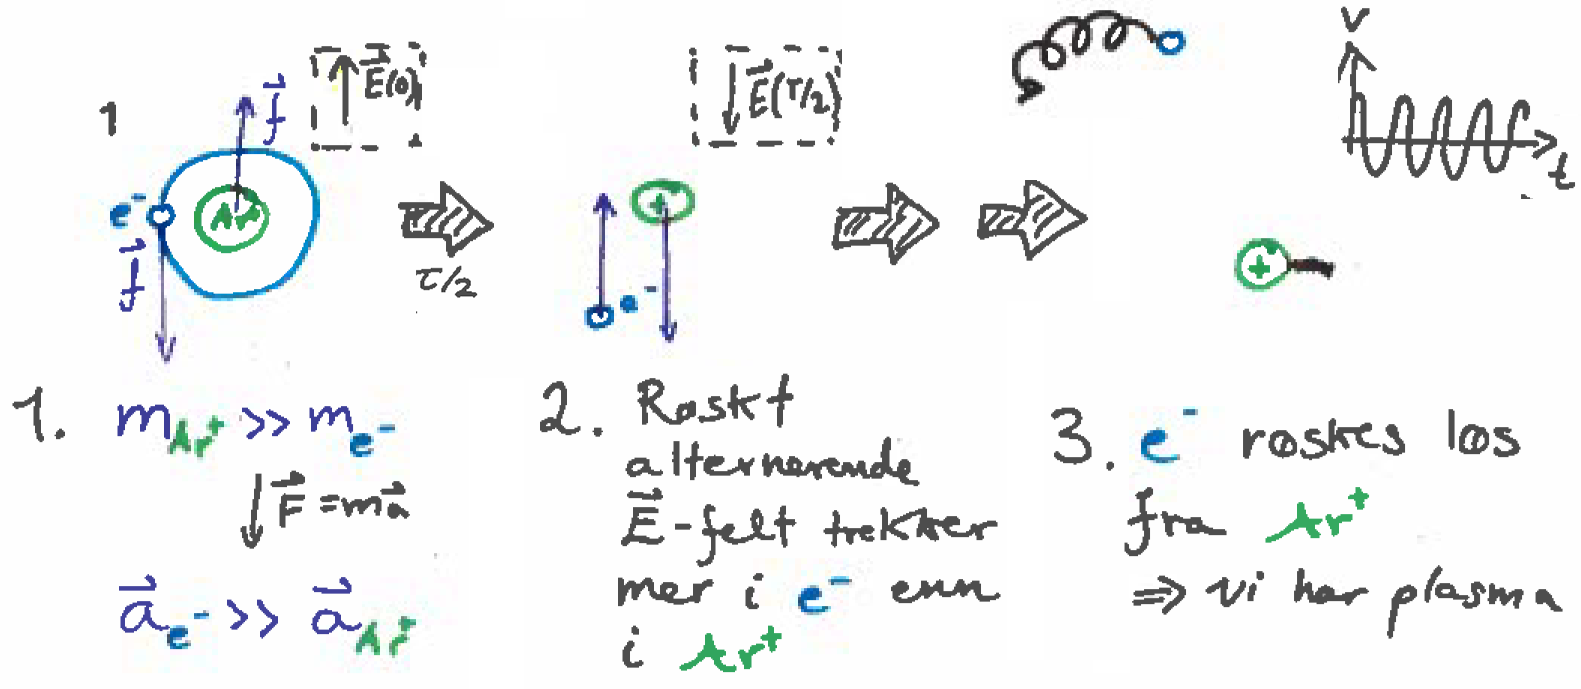
\includegraphics[width=\linewidth]{metodefigs/plasmagen.png}
\caption{Sånn kan man lage plasma. Bruk vernebriller!}
\emd\end{figure}

\paragraph{Plasma-enhanced CVD (PECVD)} I plasma-aktivert CVD lager vi plasma av gassene. De ioniserte gassene er veldig reaktive, og vi trenger derfor ikke den samme temperaturen for å oppnå reaksjonene som skal til for å lage en tynnfilm. Temperaturen er gjerne \SI{800}{\kelvin} eller lavere for PECVD.

En ytterligere fordel med PECVD er at man kan bruke et elektrisk felt til å akselerere reaktantene mot substratet, siden ionene har ladning. Dermed kan man få strukturer smo gror i én bestemt retning. Man kan for eksempel gro karbonnanorør som gror vertikalt (og ikke bare det -- man kan bestemme rollup-vektoren også!), noe som ville vært vanskelig med termisk aktivert CVD der ting gror isotropt.

\cstitle{Physical Vapor Deposition (PVD)}
PVD kort forklart: du har en blokk med materialet du vil lage tynnfilm av (denne blokken kalles ``target'' i PVD-sammenheng). Du tilfører dette kildematerialet en god bunt med energi. Energien gjør at atomer løsner fra kildematerialet. Disse atomene fanger du opp med substratet. Denne prosessen involverer som regel ikke kjemiske reaksjoner.

\paragraph{Evaporation-PVD} I evaporation-PVD tilfører du energien i form av varme:
\begin{figure}[H]
\bmd\centering
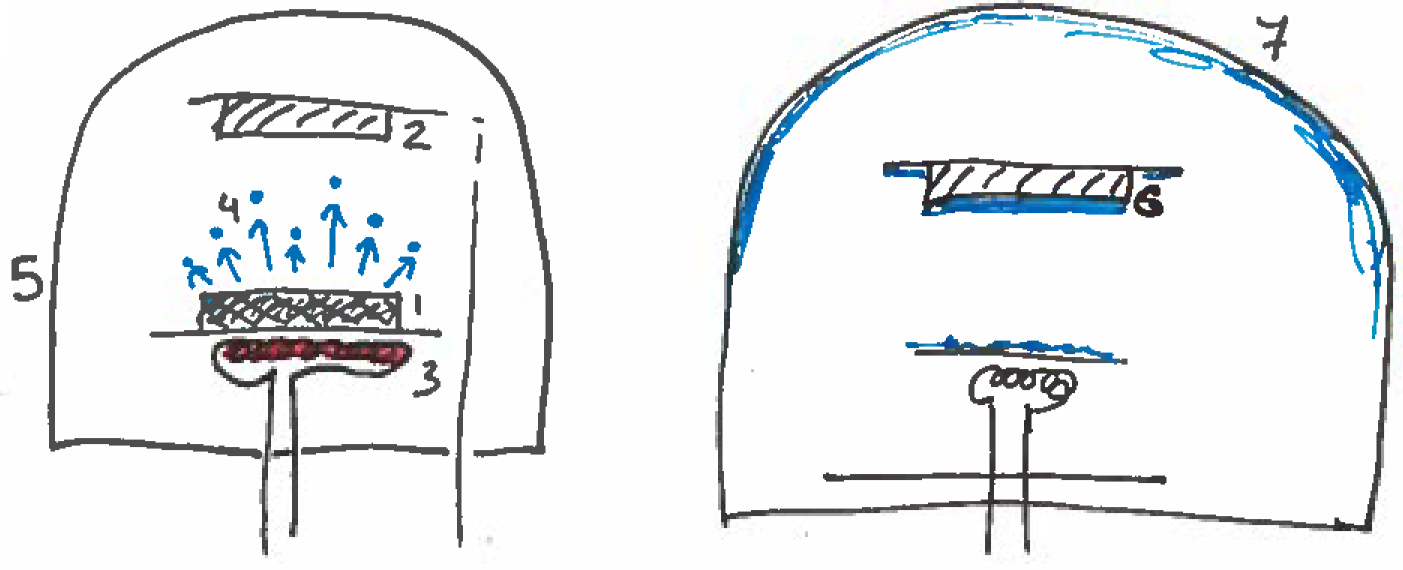
\includegraphics[width=\linewidth]{metodefigs/evappvd.png}
\caption{Sånn kan man gjøre evaporation-PVD. 1: Kilde til materialet (``target''). 2: Substrat. 3: Resistiv oppvarming av target. 4. Atomer fra kildematerialet løsner fra target ved fordamping. 5. Alt skjer inne i et vakuumkammer med trykk mellom $10^{-3}$ og $10^{-10}$ torr. 6: En film dannes på substratet. 7: En film dannes også overalt eller på utstyret :(}
\emd\end{figure}
Hvis du bare tilfører varme vil atomene fare overalt etter at de har løsnet, så hele PVD-systemet kommer til å bli dekket med tynnfilm hvis du bruker denne metoden. Det samme gjelder mange typer PVD.

\paragraph{Molecular Beam Epitaxy} er en mer fancy og sammensatt variant av evaporation-PVD, der man har flere \emph{Knudsen-celler} med hver sin blokk av kildemateriale som varmes opp på samme måte som i evaporation-PVD. MBE kjennetegnes ved et \emph{ultrahøyt vakuum}, og at atomene eller molekylene fra kildematerialet ikke interagerer med hverandre. Vekst-mekanismen i MBE blir dermed meget enkel og lett å kontrollere. Veksten skjer atomlag for atomlag, og går dermed temmelig sakte -- hastigheten til veksten er mindre enn en mikrometer i timen. Siden tynnfilmvekst med MBE er treig og kontrollerbar, brukes den til å lage tynnfilmer som er énkrystaller. Man kan også lage multikrystalline filmer med skarpe grenseflater mellom hvert lag av filmen (se figur).
\begin{figure}[H]
\bmd\centering
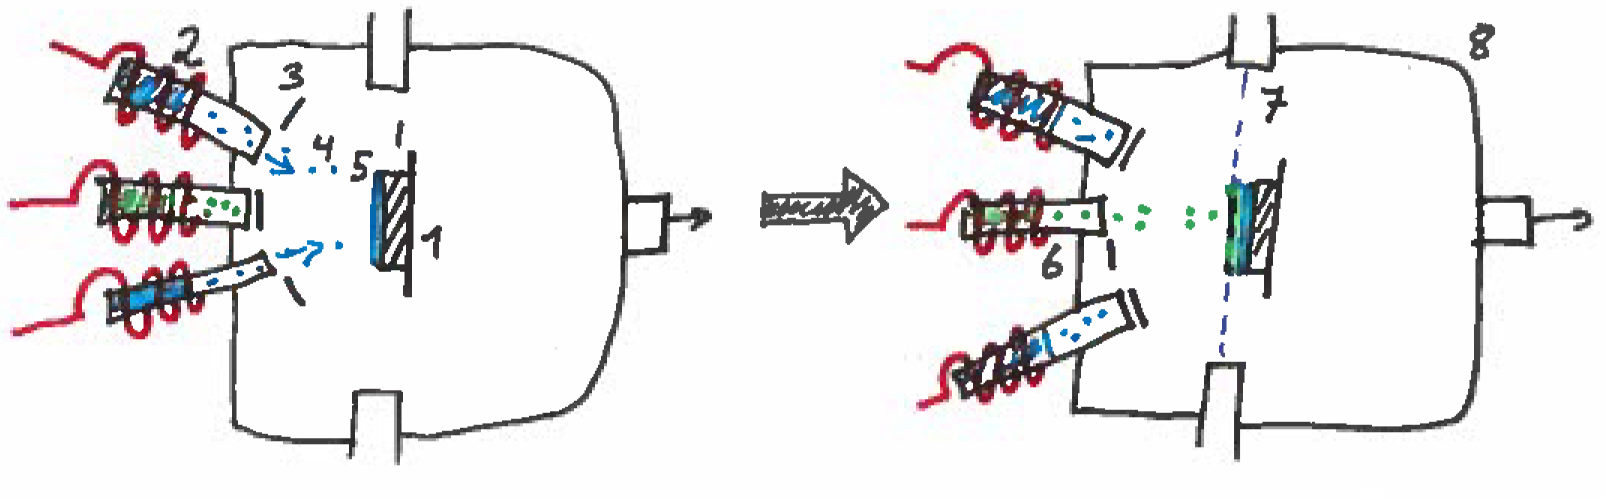
\includegraphics[width=\linewidth]{metodefigs/mbe.png}
\caption{Sånn kan man gjøre MBE. 1: Substrat. 2: Knudsen-celler -- kildematerialet varmes opp og fordamper her. 3/4: Lukkere åpner og lukkes for å kontrollere hva som når frem til substratet. 5: Det som når fram til substratet, danner en film der. 6: Bytt mellom hvilke lukkere som er åpne for å gro lagvise filmer. 7: Mulighet for \emph{in situ}-karakterisering (for eksempel RHEED). 8: vakumkammer med ultrahøyt vakuum er nødvendig i MBE.}
\emd\end{figure}
En fordel med MBE er at det er (relativt) lett å putte inn måleinstrumenter som karakteriserer materialet \emph{in situ} mens det gror. Dette gir enda bedre muligheter for å kontrollere prosessen.

\paragraph{Elektronstråle-PVD} I elektronstråle-PVD (electron beam PVD, EBPVD) er det en stråle av høyenergetiske elektroner som er energikilden. Siden elektronstrålen kan fokuseres, er det mulig å bruke materialet mer effektivt enn med andre metoder. I tillegg trenger ikke temperaturen å være særlig høy. Deponeringsraten med EBPVD er ganske høy, mellom ca. 0.1 og 100 mikrometer i \emph{minuttet}. 

I tillegg til elektronstrålen kan man bruke ionekilder til å modifisere substratet (dette gjøres \emph{etter} at elektronstrålen har blitt brukt). Dette kalles \emph{ionestråle-assistert} EBPVD. Ionestrålen kan brukes direkte til å etche eller rense substratet, kontrollere mikrostrukturen til substratet, eller til å modifisere filmen etter at den er deponert.

\paragraph{Sputtering} I sputtering bombarderes target med ioner, som gjør at atomer fra target løsner, og så treffer de substratet. Enkelt og greit.
\begin{figure}[H]
\bmd\centering
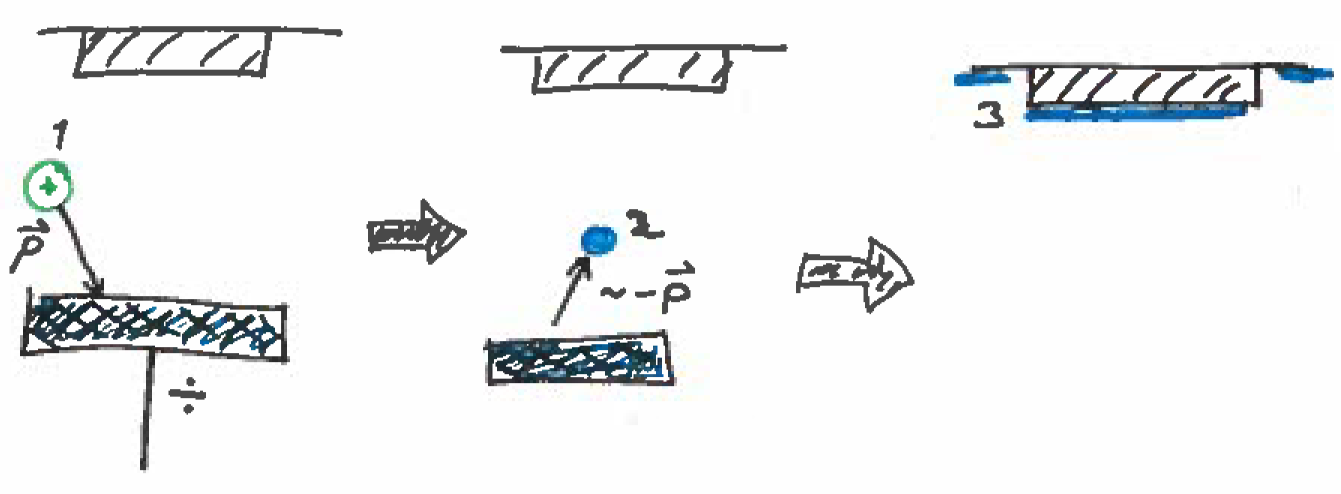
\includegraphics[width=\linewidth]{metodefigs/sputring.png}
\caption{Sputtering. 1. Argonioner fra plasma treffer target. 2: Atomer fra kilden løsner... 3: ...og dekker substratet (samt resten av utstyret) med en film.}
\emd\end{figure}

\paragraph{Cathodic sputtering} I katodisk sputring lar man target være en katode (altså holdes den ved et negativt potensial), slik at de positive ionene akselereres mot target. Dette slår løs nøytrale atomer fra target, og disse nøytrale atomene kan uten problemer komme seg på tvers av det elektriske feltet og frem til substratet.

\paragraph{Magnetron sputtering} Magnetron sputtering er en forbedring av katodisk sputring der man bruker magneter til å holde elektronene nær overflaten av target. Dette fører til høyere plasmatetthet i området rundt target,\footnote{Mulig forklaring: det er litt som hvordan radiofrekvente alternerende felt lager plasma ved at argonionene ikke klarer å holde følge med elektronene --- i dette tilfellet blir det at de magnetiske feltlinjene er sterke nok til å holde elektronene i nærheten av target, men ikke sterke nok til å holde argonionene i nærheten av target.} og det gjør også at ionene har høyere energi. Dermed for også de sputrede atomene høyere energi, slik at den resulterende filmen blir tettere og sitter bedre fast i substratet.

\paragraph{Ion beam sputtering} Med denne metoden dropper man plasma og felt og sånn, og bare skyter en ionestråle rett på target. Fordelen med denne metoden er at man kan kontrollere energien til ionene bedre (den avhenger kun av forholdene i ionestråle-generatoren), man kan ha både høy ionetetthet og en tykk stråle, og man kan gjøre deponeringen under et høyere vakuum enn man kan i plasmasputtering (som er fint hvis man av andre grunner trenger høyt vakuum).

\paragraph{Pulsed Laser Deposition (PLD)} I PLD er det ikke energetiske ioner, men en energetisk laser som treffer substratet.
\begin{figure}[H]
\bmd\centering
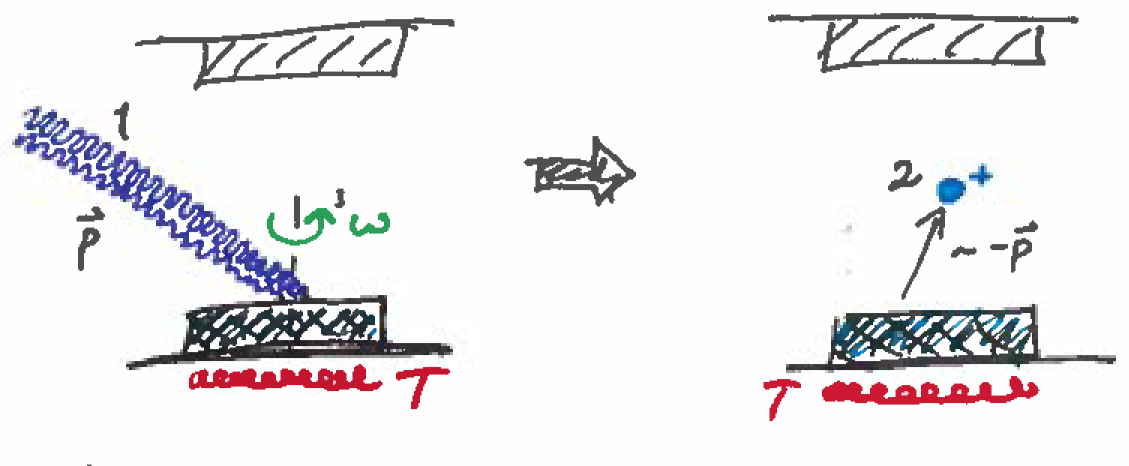
\includegraphics[width=\linewidth]{metodefigs/pld.png}
\caption{Pulsed Laser Deposition. 1: Laser treffer kilden, og feltet i laseren er nok til å røske elektronene løs fra materialet. 2: Ionisert materiale fordamper ved oppvarming. 3: Kilden kan roteres for å beskytte materialet, eller for å variere hvilket stoff som deponeres.}
\emd\end{figure}

\paragraph{Cathodic arc evaporation} I cathodic arc evaporation lager man et veldig sterkt elektrisk felt mellom target og en anode. Dette fører til en voldsom lokal temperaturøkning som gjør at materialet evaporerer her.
\begin{figure}[H]
\bmd\centering
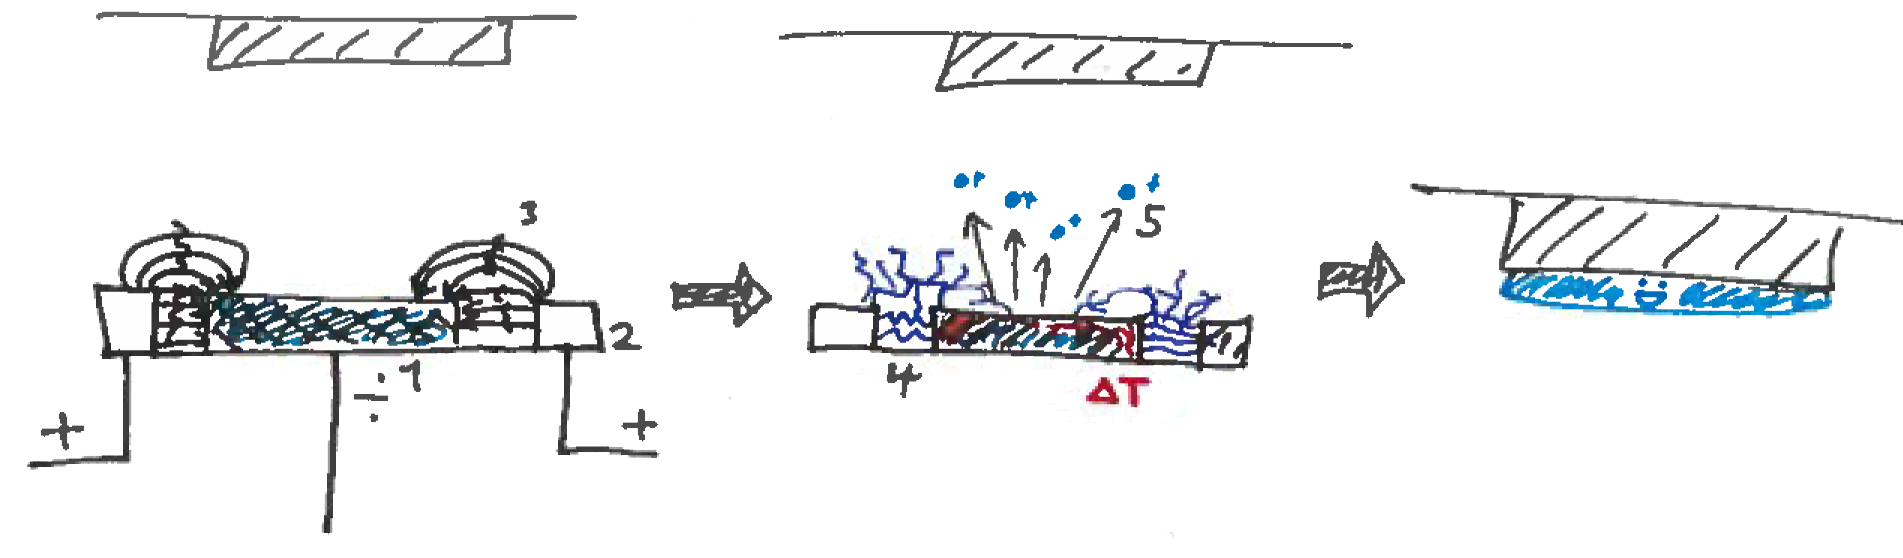
\includegraphics[width=\linewidth]{metodefigs/arcdep.png}
\caption{Cathodic arc sputtering. 1: Kilden er én elektrode. 2: Rett ved siden av kilden har man motsatt elektrode. 3: Det dannes et veldig stort lokalt $E$-felt. 4. Gjennomslag (dannelse av en lysbue) og temperaturøkning. 5: Materialet ioniseres (på grunn av lysbuen) og fordamper (på grunn av temperaturøkningen).}
\emd\end{figure}

%!TEX root = Nanomat.tex
\ctitletwo{Nanotoksikologi}
\addcontentsline{toc}{section}{NANOTOKSIKOLOGI}
Nanotoksikologi handler om hvordan materialer kan bli giftige når de er i form av ultrafine partikler. Dette området er i dag (2015) preget av at det har blitt gjort veldig lite forskning på nanotoksikologi.

\cstitletwo{Hvorfor kan nanopartikler være skadelige?}
\paragraph{Nanopartikler er små} Det har seg slik at nanopartikler er små. Det er i hovedsak to aspekter ved dette som kan gjøre dem skadelige. Det første er ganske enkelt at de kan komme seg inn på steder der større partikler ikke får tilgang. Det andre er, som vi har sett mange ganger tidligere, at materialer blir mer reaktive av å være i nanopartikkelform, fordi de får større overflate per enhet volum. Denne økte reaktiviteten gjør at giftige materialer kan bli enda giftigere i nanopartikkel-form. Andre faktorer som kan spille en rolle er endringer i materialenes egenskaper (løselighet, form, ledningsevne) når partiklene blir veldig små.

\paragraph{Det vi vet så langt: direkte eksponering} Det som har blitt gjort av forskning, handler for det meste om effektene av direkte eksponering til nanopartikler. Nanopartikler penetrerer og angriper faktisk deler av levende organismer som større partikler ikke kommer frem til. Dette har man funnet ut ved å pumpe \ce{TiO2}-partikler direkte inn i luftveiene til rotter og mus. Partikler med diameter på \SI{20}{\nano\meter} førte til en langt større grad av betennelse (målt som konsentrasjon av hvite blodceller) enn partikler med diameter på \SI{250}{\nano\meter}, per gram \ce{TiO2}. Hvis man ser på grad av betennelse målt mot det samlede overflatearealet av \ce{TiO2}, så ser det ikke ut til å ha noe å si hvor store partiklene er.

I studiene som har blitt gjort så langt er ofte dosene mye høyere enn det er realistisk å oppleve i virkeligheten -- de er store nok til å fullstendig overvelde organismenes forsvarsmekanismer. Sannsynligvis vil organismer reagere kvalitativt annerledes på lave doser av nanopartikler.

\paragraph{Det vi ikke vet: effekt på miljøet} Hvilken effekt har nanopartikler på miljøet --- i jorden, planter, dyr og mennesker? Hvilke risikoer oppstår når nanopartikler fra forbrukervarer lekker ut i miljøet og senere når oss på mer indirekte vis? Hvordan og hvor i økosystemene akkumulerer nanopartikler? Hvordan kan de degraderes?

\vfill
\columnbreak

\cstitletwo{Eksponeringsveier}
Hvordan kan nanopartikler komme seg inn i oss?
\begin{itemize}
	\item \emph{Inhalering} av luftbårne partikler er den viktigste eksponeringsveien, og også den som det har blitt forsket mest på. Partikler med størrelse på ca. \SI{1}{\micro\meter} er de som går lettest gjennom nesa/svelget (større partikler blir blokkert, mindre partikler blir absorbert) og inn i luftrøret og videre inn i lungene.
	\item \emph{Opptak gjennom huden}: nanopartikler kan komme seg gjennom huden enten ved å gå gjennom cellene, ved å gå mellom cellene eller å gå inn langs hårsekkene. Det har blitt vist at nanopartikler kan komme seg inn i blodet og nervesystemet hvis de først kommer gjennom huden. Mange kosmetiske produkter inneholder nanopartikler, men disse er trolig for store til å penetrere huden. Men hva om de brukes på sprukket hud og sår?
	\item \emph{Inntak gjennom mat og drikke}: det har bare blitt gjort noen få studier på inntak av nanomaterialer gjennom fordøyelsessystemet, men det ser ut til at de går rett gjennom og elimineres raskt.
	\item \emph{Injeksjon}: hvis nanopartikler skal brukes til drug delivery, vil naturligvis injeksjon direkte inn i blodet være en eksponeringsvei for nanopartikler.
\end{itemize}

\cstitletwo{Risikovurdering av nanopartikler}
Per 2015 har man dessverre ikke klart å gjøre noe særlig systematisk utredning av risiko knyttet til nanomaterialer og -partikler. Dermed har man ikke grunnlag for å gjøre en tilstrekkelig risikovurdering. 

Om man ikke skal stoppe forskning på nanoteknologi og nanopartikler helt for å være føre var, bør man i hvert fall gjøre en tilstrekkelig innsats i å identifisere og minimere faremomenter. De som produserer nanomaterialer må være klar over hvilken risiko som er forbundet med nanomaterialer, og de må kunne vise at produktene de lager, er trygge nok. Hvis dette ikke blir demonstrert i tilstrekkelig grad, vil offentligheten se på nanomaterialer som farlige, noe som kan føre til feilkarakterisering og unødvendig streng regulering av nanoprodukter. Dette vil igjen være en hindring for forskning på, og kommersialisering av, nanomaterialer.

\ifbool{multicol}{\end{multicols}}{}

%\appendix
\centerline{\color{Orange}\Huge{Appendiks}}
\begin{changemargin}{2.5cm}{2.5cm}
\section{Bariumtitanat og ferroelektriske tynnfilmer}
\index{ferroelektrisitet}\index{tynnfilmer}\index{bariumtitanat}\index{polarisering}\index{perovskitt}
Et spørsmål man kan gruble over når man leser om endringen i krystallstrukturen til \ce{BaTiO3}, er: hvordan bestemmer \ce{Ti^4+} seg for om den skal gå opp eller ned, når situasjonen er helt symmetrisk over overgangstemperaturen? Svaret fant jeg først etter å ha sendt to meldinger til Reddit-brukeren ``troixetoiles'', som jobber med ferroelektriske tynnfilmer. Hun sendte meg også en forholdsvis utdypende forklaring av hva som skjer i \ce{BaTiO3}, så jeg legger ved samtalen vår her (minus høflighetsfraser).

\paragraph{According to what I've read, this effect ({\ttfamily https://i.imgur.com/75M9M.png}) happens spontaneously when the material is cooled below \SI{120}{\celsius}. I can understand that this would happen if one also applies an electric field as the material cools, but doesn't it also happen in the absence of an external electric field? Does it happen in a specific direction ($P_{\text{up}}$ or $P_{\text{down}}$) every time? If so, what in the world gives rise to that asymmetry in an apparently perfectly symmetric situation?} \mbox{}\\

\noindent So the effect in the picture is the change in crystal structure and symmetry and the accompanying ferroelectric phase transition that happens below the transition temperature. You are right in that it does happens in the absence of an electric field because ferroelectric materials all have a naturally occurring ``spontaneous'' electric polarization, which means it exists in zero field.

Essentially the simplest way to think about what this is (or how I think about it) is a distortion away from the cubic case, which is centrosymmetric. There are two main distortions to the \ce{BaTiO3} unit cell when it become ferroelectric, one is that it elongates in the direction of the polarization, and the other is that the \ce{Ti} atom displaces. Since each atom is really a cation or anion, the displacement of the \ce{Ti} atom causes charges to be displaces from symmetric positions, which leads to the development of a dipole moment in the unit cell. When you add this up over a large number of unit cells in a crystal, then you have a macroscopic ferroelectric polarization.

The question of whether the polarization is constrained to two directions (e.g. $P_{\text{up}}$ and $P_{\text{down}}$) is a good one. And the answer depends on the material system you are talking about. If you look at the drawing above, you probably realize you can rotate the middle or right drawing and get the same structure with P pointed in the four in-plane directions, so you could also get $P_{\text{left}}$ or $P_{\text{right}}$, $P_{\text{front}}$, or $P_{\text{back}}$. In a bulk crystal each of these directions is equally valid because it's all the same distortion of the cubic cell, just in different directions, so in the absence of an electric field one shouldn't be preferred over the others.

A lot of ferroelectric work is done on thin films, however, and this is a different case. For thin films, you grow a very thin (\SIrange{10}{20}{\nano\meter} for example) layer of \ce{BaTiO3} on top of a substrate that usually has the same basic cubic structure but may have different lattice parameters. In a system like this, the in-plane unit cell size of the \ce{BaTiO3} layer is constrained to that of the substrate. So take a system like \ce{BaTiO3} grown on SrTiO3. SrTiO3 has a smaller lattice parameter than \ce{BaTiO3}, so when you grow the latter material on top of the former, you are forcing the in-plane sides of the \ce{BaTiO3} structure to compress in a little bit to match the size of the \ce{SrTiO3} unit cell. This leads to an expansion in the out-of-plane direction that will match what you see in the image you attached. This then constrains the polarization to be in one of two directions: up or down.

Not onto your last query: why would a nicely symmetric system become not-as-symmetric and why would a ferroelectric polarization develop? My studies have been in ferroelectrics similar to \ce{BaTiO3} so I can best speak to materials with the same type of crystal structure. The structure above is called the perovskite structure. You can apply something called a Goldschmidt tolerance factor to these systems, which is an equation that takes the radii of each of the types of atom in the structure and computes how stable the structure is. Depending of the relative sizes of the non-oxygen atoms, structures can be more of less stable, so for \ce{BaTiO3}, at room temperature the \ce{Ti} atom is ``too big'' for the nice cubic structure to be stable. I haven't thought too much about the phase transition between the two states but my first guess at an explanation from this angle would be that due to thermal expansion, as the temperature rises there is more room to accommodate the \ce{Ti} atom so at some point a more symmetric, cubic structure can be stabilized.

\paragraph{What I'm really wondering about is whether the polarization is consistently in one particular direction (say, up) and not the other (down). Because it seems like you could flip that system vertically and get the same structure above the transition temperature, but then below the transition temperature, the \ce{Ti} would go in the opposite direction from what it did last time - even though the conditions didn't actually change.} \mbox{}\\

\noindent You are right in that both directions are equally as favorable energetically. In realistic systems you sometimes have states where the entire sample is in the same polarization, but more often you have cases where the system is in different polarization domains, so different areas of the system are polarized in certain directions. With thin films, as I mentioned before, you are usually constrained to $P_{\text{up}}$ and $P_{\text{down}}$ so you can get areas with both, although the exactly configuration depends on film thickness. That's because if you have these domains, there are walls between them, so you need to figure out which case is more energetically favorable: a single domain, or multiple domains with walls that cost energy. You also need to take other electrostatic stuff into account, too, so it can get a bit complicated, but the take home message is that a system with different polarization domains is very common.

I don't know what journals you have access to, but this is a pretty cool paper on these domains in films thin ferroelectric films where you can get an idea of what they look like: {\ttfamily http://scitation.aip.org/content/aip/journal/apl/93/18/10.1063/1.3013512}

Often in bulk, say in large crystals, you may get domains where the structure goes tetragonal (basically becomes elongated) in different directions, so you can also get different polarization domains. Again, I can't speak to this as much, but with early studies on bulk ferroelectric materials you can get good examples for this.

Once you apply an electric field, however all the polarization wants to align with it, so you create a monodomain state.

I just realized now you also asked about this structure above and below the transition temperature. Above that temperature, the system is no longer in the distorted state. It is cubic and centrosymmetric, so it looks like the leftmost figure in the original picture. Since there are no atomic displacements, there is no polarization. In the original picture the middle and right images are the two stable states below the transition temperature.

\paragraph{So it's pretty much exactly like how you have magnetic domains in ferromagnetic materials? That makes sense. I had the impression that the entire material would somehow polarize as a single domain.} \mbox{}\\
\index{Kittels lov}
\noindent Yep, pretty much the same basic formalism can be used to describe ferroelectric and ferromagnetic domains (Kittel's law). The sizes and energy considerations are different, however, since ferroelectric domain walls tend to be a lot thinner than magnetic ones and other energetics are different, as well, but the two are pretty analogous.

\end{changemargin}

